%
% Qucs Functions Reference Manual
%
% Copyright (C) 2006 Gunther Kraut <gn.kraut@t-online.de>
%
% Permission is granted to copy, distribute and/or modify this document
% under the terms of the GNU Free Documentation License, Version 1.1
% or any later version published by the Free Software Foundation.
%

\setlength\parskip{12pt}

\tutsection{Introduction}
This manual describes the measurement expressions available in
\char`\"{}Qucs\char`\"{}, the \char`\"{}Quite Universal Circuit
Simulator\char`\"{}.

Measurement expressions come into play whenever the results of a
\char`\"{}Qucs\char`\"{} simulation run need post processing. Examples
would be the conversion of a simulated voltage waveform from volts to
dBV, the root mean square value of that waveform or the determination
of the peak voltage. The
\char`\"{}Qucs\char`\"{} measurement functions offer a rich set of
data manipulation tools.

If you are not familiar with the way how to enter those formulas,
please refer to chapter \textit{``\nameref{chapter:use}''}, which
points out the possibilities to create and change measurement
expressions. Also the data types supported are specified here. Chapter
\textit{``\nameref{chapter:syntax}''} introduces the basic syntax of
functions and a categorical list of all functions available. The core
of the document, a detailed compilation of all ''Qucs'' functions
divided into different categories, is presented in chapter
\textit{``\nameref{chapter:math}''} and chapter
\textit{``\nameref{chapter:electronics}''}.  Finally, the
\textit{\hyperlink{chapter:appendix}{Index}} contains an alphabetical list
of all functions.


\tutsection{\label{chapter:use}Using Measurement Expressions}
%%%%%%%%%%%%%%%%%%%%%%%%%%%%%% LyX specific LaTeX commands.
%% Bold symbol macro for standard LaTeX users
\providecommand{\boldsymbol}[1]{\mbox{\boldmath $#1$}}

%% Because html converters don't know tabularnewline
\providecommand{\tabularnewline}{\\}

\tutsubsection{Entering Measurement Expressions}

Measurement expressions generate new datasets by function or operator
driven evaluation of simulation results. Those new datasets are accessible
in the data display tab. The related equations can be entered into
the schematic editor by the following means:

\begin{itemize}
\item Using the equation icon in the {}``Tools'' bar (see fig. \ref{cap:Entering})
\item Using menu item {}``Insert'' $\rightarrow$ ''Insert equation''
\end{itemize}
%
\begin{figure}[ht]
\begin{center}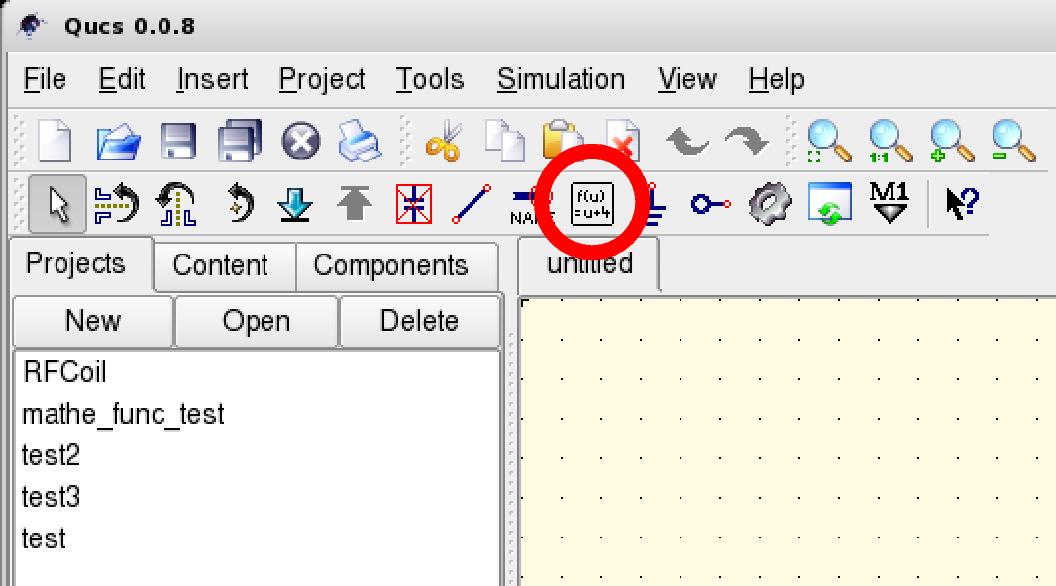
\includegraphics[%
  scale=0.4]{qucs_formula1}\end{center}


\caption{\label{cap:Entering}Entering a new measurement expression via equation
icon}
\end{figure}


\noindent You can now place the equation symbol by mouse click anywhere
in the schematic. Each mouse click creates a new equation instance.
Press the <ESC> key if you do not like further equations.

Another option is to select an existing equation, copy it (either
by menu item {}``Edit'' $\rightarrow$ ''Copy'' or by <CTRL>+C%
\footnote{<CTRL>+C means that you have to press the <CTRL> key and the C key
simultaneously.%
}) and paste it (either by menu item {}``Edit'' $\rightarrow$ ''Paste'' or
by <CTRL>+V).

After having successfully created an equation, you are now able to
modify it.


\tutsubsection{Changing Measurement Expressions}

For sake of simplicity we assume that you have just generated a new
equation - if you like to change an existing, more complicated equation
the following steps are the same.

Thus, the excerpt of your schematic surface looks like that in fig.
\ref{cap:Newly-created-equation}.

%
\begin{figure}[ht]
\begin{center}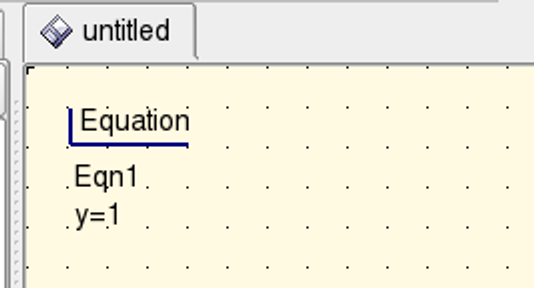
\includegraphics[%
  scale=0.4]{qucsformula2.png}\end{center}


\caption{\label{cap:Newly-created-equation}Newly created equation}
\end{figure}


You can now manipulate the current name of the equation. Simply click
onto {}``Eqn1'', which becomes highlighted. Then type in a new name
for it and finalise your inputs with the <RETURN> key.

After that, you can enter a new equation. Again, click onto {}``y=1''.
Only the {}``1'' is marked, and you can enter a new expression there.
Please use the variables, operators and constants described in chapter
\ref{sec:Syntax}. Note that you can also refer to results (dependents)
of other equations. But how to change the name of the current dependent
{}``y'' ? Right click onto the equation, and a context menu opens.
Select the first item called {}``Edit properties''. A sub window
appears, which should look like the one in fig. \ref{cap:Editing-equation-properties}.
The alternative for entering equations is to double click onto the
equation.

%
\begin{figure}
\begin{center}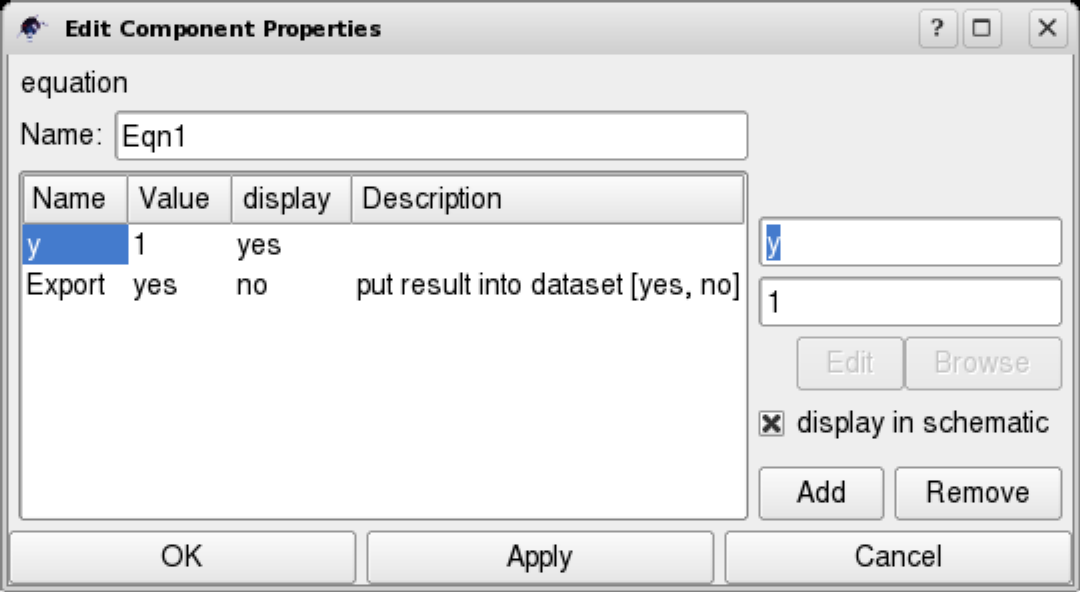
\includegraphics[%
  scale=0.4]{qucsformula3.png}\end{center}


\caption{\label{cap:Editing-equation-properties}Editing equation properties}
\end{figure}


You can now change the name of the dependent, the equation itself
(which is {}``1'' in the example shown) and the name of the equation.
If you do not want the result to be exported into the data display
tab, but temporarily need it for further calculations, select {}``no''
in the {}``Export value'' cell. 


\tutsubsection{\label{sec:Syntax}Syntax of Measurement Expressions}

Function names, variable names, and constant names are all case sensitive
in measurement expressions - it is distinguished between lowercase
and uppercase letters such as 'a' and 'A'.

\noindent In functions, commas are used to separate arguments.


\tutsubsubsection{Variable Names}

User defined variable names consist of a letter, followed by any number
of letters, digits, or underscores.

The syntax of variable names created by the \char`\"{}Qucs\char`\"{}
simulator is as specified in table \ref{table:var_names}. Please
note that all voltages and currents in {}``Qucs'' are peak values.

%
\begin{table}[ht]
\begin{flushleft}\begin{tabular}{|r|l|}
\hline 
Variable Name&
Description\tabularnewline
\hline
\hline 
\textit{nodename}.V&
DC voltage at node \textit{nodename}\tabularnewline
\hline 
\textit{name}.I&
DC current through circuit component \textit{name}\tabularnewline
\hline 
\textit{nodename}.v&
AC voltage at node \textit{nodename}\tabularnewline
\hline 
\textit{name}.i&
AC current through circuit component \textit{name}\tabularnewline
\hline 
\textit{nodename}.vn&
AC noise voltage at node \textit{nodename}\tabularnewline
\hline 
\textit{name}.in&
AC noise current through circuit component \textit{name}\tabularnewline
\hline 
\textit{nodename}.Vt&
Transient voltage at node \textit{nodename}\tabularnewline
\hline 
\textit{name}.It&
Transient current through circuit component \textit{name}\tabularnewline
\hline
\textit{name}.OP&
\textit{name} = component name, OP = operating point (device dependent),\tabularnewline
&
 e.g. D1.Id\tabularnewline
\hline
S{[}x,y{]}&
S-parameter, e.g. S{[}1,1{]}\tabularnewline
\hline
Rn&
equivalent noise resistance\tabularnewline
\hline
Sopt&
optimal reflection coefficient for minimum noise\tabularnewline
\hline
Fmin&
minimum noise figure\tabularnewline
\hline
F &
noise figure\tabularnewline
\hline
\textit{nodename}.Vb&
Harmonic balance voltage at node \textit{nodename}\tabularnewline
\hline 
\end{tabular}\end{flushleft}


\caption{\label{table:var_names}Syntax of simulator generated variable names}
\end{table}



\tutsubsubsection{Numbers}

Numbers are written in conventional decimal way, with an optional
decimal point between the digits. For powers of ten, the familiar
scientific notation with an 'e' is used. In this way, '1.234e6' is an
example for the real floating point number 1234000. Imaginary numbers
can be entered by a multiplication factor 'i' or 'j' (see also table
\ref{table:constants}).  An example would be '1+2{*}i' or - if you
want to leave out the multiplication sign - '1+i2'.


\tutsubsubsection{Built-in constants}

The constants which can be used within measurement expressions are
given in table \ref{table:constants}.

%
\begin{table}[ht]
\begin{center}\begin{tabular}{|c|c|c|}
\hline 
Operator&
Description&
Value\tabularnewline
\hline
\hline 
e&
Euler's constant&
2.718282\tabularnewline
\hline 
i , j&
Imaginary unit $\left(\sqrt{-1}\,\right)$&
i1\tabularnewline
\hline 
kB&
Boltzmann's constant&
1.380658e23 J/K\tabularnewline
\hline 
pi&
$\pi$&
3.141593\tabularnewline
\hline
\end{tabular}\end{center}


\caption{\noindent \label{table:constants}Built-in Constants}
\end{table}



\tutsubsubsection{Operators}


\tutparagraph{Operator Precedence}

Expressions are evaluated in the standard way, meaning from left to
right, unless there are parentheses. The priority of operators is
also handled familiarly, thus for example multiplication has precedence
to addition. Table \ref{table:operators} specifies a sorted list
of all operators, the topmost having highest priority. Operators on
the same line have the same precedence.

%
\begin{table}[ht]
\begin{center}\begin{tabular}{|c|c|c|}
\hline 
Operator&
Name&
Example\tabularnewline
\hline
\hline 
()&
Parentheses, function call&
max(v)\tabularnewline
\hline 
\textasciicircum{}&
Exponentiation&
3\textasciicircum{}4\tabularnewline
\hline 
{*}&
Multiplication&
3{*}4\tabularnewline
/&
Division&
3/4\tabularnewline
\%&
Modulo&
4\%3\tabularnewline
\hline 
+&
Addition&
3+4\tabularnewline
-&
Subtraction&
3-4\tabularnewline
\hline 
:&
Range operator&
3:12\tabularnewline
\hline
\end{tabular}\end{center}


\caption{\label{table:operators}Operator priorities}
\end{table}



\tutparagraph{Ranges}

The general nomenclature of ranges is displayed in table \ref{table:Range-definition}.
It shows one-dimensional ranges, whereas also n-dimensional ranges
are possible, if you consider nested sweeps.

%
\begin{table}
\begin{center}\begin{tabular}{|c|c|}
\hline 
Syntax&
Explanation\tabularnewline
\hline
\hline 
m:n&
Range from index \textit{m} to index \textit{n}\tabularnewline
\hline 
:n&
Range up to index \textit{n}\tabularnewline
\hline 
m:&
Range starting from index \textit{m}\tabularnewline
\hline 
:&
No range limitations\tabularnewline
\hline
\end{tabular}\end{center}


\caption{\label{table:Range-definition}Range definition}
\end{table}



\tutsubsubsection{Post Processing of Simulation Data by Expressions}

After a simulation has run the results are stored in datasets. Usually,
such a dataset is a vector or a matrix, but may also be a real or
complex scalar. For transient analysis, this dataset contains voltage
or current information over time, for Harmonic Balance it contains
amplitudes at dedicated frequencies, while for S-parameter analysis
a vector of matrices (thus matrices in dependency of frequency) is
returned. In further generalisation the components of vectors and
matrices consist of complex numbers.

Additionally, datasets can be generated by using expressions. As an
example the linspace() function shall be named, which creates a vector
of linearly spaced elements.


\tutsection{\label{chapter:syntax}Functions Syntax and Overview}
%%%%%%%%%%%%%%%%%%%%%%%%%%%%%% LyX specific LaTeX commands.
%% Bold symbol macro for standard LaTeX users
\providecommand{\boldsymbol}[1]{\mbox{\boldmath $#1$}}

%% Because html converters don't know tabularnewline
\providecommand{\tabularnewline}{\\}

This chapter introduces the basic syntax of the function descriptions
and contains a categorical list of all available functions.

\tutsubsection{Functions Reference Format}

\char`\"{}Qucs\char`\"{} provides a rich set of functions, which can
be used to generate and display new datasets by function based evaluation
of simulation results. Beside a large number of mathematical standard
functions such as square root (sqrt), exponential function (exp),
absolute value (abs), functions especially useful for calculation
and transformation of electronic values are implemented. Examples
for the latter would be the conversion from Watts to dBm, the generation
of noise circles in an amplifier design, or the conversion from S-parameters
to Y-parameters.


\tutsubsubsection{Functions Reference Format}

In the subsequent two chapters, each function is described using the
following structure: 

\begin{description}
\item [<Function~Name>]~
\end{description}
Outlines briefly the functionality of the function.

\begin{description}
\item [Syntax]~
\end{description}
Defines the general syntax of this function.

\begin{description}
\item [Arguments]~
\end{description}
Name, type, definition range and whether the argument is optional,
are tabulated here. In case of an optional parameter the default value
is specified. {}``Type'' is a list defining the arguments allowed
and may contain the following symbols:
\medskip{}

\begin{tabular}{|c|c|}
\hline 
Symbol&
Description\tabularnewline
\hline
\hline 
$\mathbb{R}$&
Real number\tabularnewline
\hline 
$\mathbb{C}$&
Complex number\tabularnewline
\hline 
$\mathbb{R}^{n}$&
Vector consisting of \textit{n} real elements\tabularnewline
\hline 
$\mathbb{C}^{n}$&
Vector consisting of \textit{n} complex elements\tabularnewline
\hline
$\mathbb{R}^{m\times n}$&
Real matrix consisting of \textit{m} rows and \textit{n} columns\tabularnewline
\hline
$\mathbb{\mathbb{C}}^{m\times n}$&
Complex matrix consisting of \textit{m} rows and \textit{n} columns\tabularnewline
\hline
$\mathbb{R}^{m\times n\times p}$&
Vector of \textit{p} real $m\times n$ matrices\tabularnewline
\hline
$\mathbb{\mathbb{C}}^{m\times n\times p}$&
Vector of \textit{p} complex $m\times n$ matrices\tabularnewline
\hline
\end{tabular}

\medskip{}
{}``Definition range'' specifies the allowed range. Each range is
introduced by a bracket, either {}``$\left[\right.$'' or {}``$\left]\right.$'',
meaning that the following start value of the range is either included
or excluded. The start value is separated from the end value by a
comma. Then the end value follows, finished by a bracket again, either
{}``$\left[\right.$'' or {}``$\left]\right.$''. The first bracket
mentioned means {}``excluding the end value'', the second means
{}``including''.
\vspace{12pt}

If a range is given for a complex number, this specifies the real
or imaginary value of that number. If a range is given for a real
or complex vector or matrix, this specifies the real or imaginary
value of each element of that vector or matrix. The symbols mean {}``includes
listed value'' and {}``excludes listed value''.

\begin{description}
\item [Description]~
\end{description}
Gives a more detailed description on what the function does and what
it returns. In case some background knowledge is presented.

\begin{description}
\item [Examples]~
\end{description}
Shows an application of the function by one or several simple examples.

\begin{description}
\item [See~also]~
\end{description}
Shows links to related functions. A mouse click onto the desired link
leads to an immediate jump to that function.


\tutsubsection{Functions Listed by Category}

This compilation shows all {}``Qucs'' functions sorted by category (an alphabetical list is given in the \hyperlink{chapter:appendix}{appendix}). 
Please click on the desired function to go to its detailed description.


\tutsubsubsection{Math Functions}


\subsubsection*{\nameref{sec:Vectors-and-Matrices}: \nameref{sub:Creation}}

\textcolor{blue}{}\begin{tabular}{>{\raggedleft}p{3cm}>{\centering}p{0.5cm}l}
\textcolor{blue}{\hyperlink{eye}{eye()}}&
...&
 \begin{NoHyper} \nameref{par:identity} \end{NoHyper}\tabularnewline
\textcolor{blue}{\hyperlink{linspace}{linspace()}}&
...&
 \begin{NoHyper} \nameref{par:linspace} \end{NoHyper}\tabularnewline
\textcolor{blue}{\hyperlink{logspace}{logspace()}}&
...&
 \begin{NoHyper} \nameref{par:logspace} \end{NoHyper}\tabularnewline
\end{tabular}


\subsubsection*{\nameref{sec:Vectors-and-Matrices}: \nameref{sub:Basic-Matrix-Functions}}

\textcolor{blue}{}\begin{tabular}{>{\raggedleft}p{3cm}>{\centering}p{0.5cm}l}
\textcolor{blue}{\hyperlink{adjoint}{adjoint()}}&
...&
 \begin{NoHyper} \nameref{par:Adjoint-matrix.} \end{NoHyper}\tabularnewline
\textcolor{blue}{\hyperlink{array}{array()}}&
...&
 \begin{NoHyper} \nameref{par:array} \end{NoHyper}\tabularnewline
\textcolor{blue}{\hyperlink{det}{det()}}&
...&
 \begin{NoHyper} \nameref{par:Determinant} \end{NoHyper}\tabularnewline
\textcolor{blue}{\hyperlink{inverse}{inverse()}}&
...&
 \begin{NoHyper} \nameref{par:Matrix-inverse} \end{NoHyper}\tabularnewline
\textcolor{blue}{\hyperlink{transpose}{transpose()}}&
...&
 \begin{NoHyper} \nameref{par:Matrix-transpose} \end{NoHyper}\tabularnewline
\textcolor{blue}{\hyperlink{length}{length()}}&
...&
 \begin{NoHyper} \nameref{par:Vector-length} \end{NoHyper}\tabularnewline
\end{tabular}


\subsubsection*{\nameref{sec:Elementary-Mathematical-Functions}: \nameref{sub:Basic-Real-and}}

\textcolor{blue}{}\begin{tabular}{>{\raggedleft}p{3cm}>{\centering}p{0.5cm}l}
\textcolor{blue}{\hyperlink{abs}{abs()}}&
...&
 \begin{NoHyper} \nameref{par:Absolute-value} \end{NoHyper}\tabularnewline
\textcolor{blue}{\hyperlink{angle}{angle()}}&
...&
 \begin{NoHyper} \nameref{par:angle} \end{NoHyper}\tabularnewline
\textcolor{blue}{\hyperlink{arg}{arg()}}&
...&
 \begin{NoHyper} \nameref{par:arg} \end{NoHyper}\tabularnewline
\textcolor{blue}{\hyperlink{conj}{conj()}}&
...&
 \begin{NoHyper} \nameref{par:Conjugate} \end{NoHyper}\tabularnewline
\textcolor{blue}{\hyperlink{deg2rad}{deg2rad()}}&
...&
 \begin{NoHyper} \nameref{par:deg2rad} \end{NoHyper}\tabularnewline
\textcolor{blue}{\hyperlink{hypot}{hypot()}}&
...&
 \begin{NoHyper} \nameref{par:hypot} \end{NoHyper}\tabularnewline
\textcolor{blue}{\hyperlink{imag}{imag()}}&
...&
 \begin{NoHyper} \nameref{par:Imag} \end{NoHyper}\tabularnewline
\textcolor{blue}{\hyperlink{mag}{mag()}}&
...&
 \begin{NoHyper} \nameref{par:Magnitude} \end{NoHyper}\tabularnewline
\textcolor{blue}{\hyperlink{norm}{norm()}}&
...&
 \begin{NoHyper} \nameref{par:norm} \end{NoHyper}\tabularnewline
\textcolor{blue}{\hyperlink{phase}{phase()}}&
...&
 \begin{NoHyper} \nameref{par:Phase} \end{NoHyper}\tabularnewline
\textcolor{blue}{\hyperlink{polar}{polar()}}&
...&
 \begin{NoHyper} \nameref{par:polar} \end{NoHyper}\tabularnewline
\textcolor{blue}{\hyperlink{rad2deg}{rad2deg()}}&
...&
 \begin{NoHyper} \nameref{par:rad2deg} \end{NoHyper}\tabularnewline
\textcolor{blue}{\hyperlink{real}{real()}}&
...&
 \begin{NoHyper} \nameref{par:Real} \end{NoHyper}\tabularnewline
\textcolor{blue}{\hyperlink{signum}{signum()}}&
...&
 \begin{NoHyper} \nameref{par:Signum} \end{NoHyper}\tabularnewline
\textcolor{blue}{\hyperlink{sign}{sign()}}&
...&
 \begin{NoHyper} \nameref{par:Sign} \end{NoHyper}\tabularnewline
\textcolor{blue}{\hyperlink{sqr}{sqr()}}&
...&
 \begin{NoHyper} \nameref{par:Square} \end{NoHyper}\tabularnewline
\textcolor{blue}{\hyperlink{sqrt}{sqrt()}}&
...&
 \begin{NoHyper} \nameref{par:Square-root} \end{NoHyper}\tabularnewline
\textcolor{blue}{\hyperlink{unwrap}{unwrap()}}&
...&
 \begin{NoHyper} \nameref{par:Unwrap} \end{NoHyper}\tabularnewline
\end{tabular}


\subsubsection*{\nameref{sec:Elementary-Mathematical-Functions}: \nameref{sub:Exponential-and-Logarithmic}}

\textcolor{blue}{}\begin{tabular}{>{\raggedleft}p{3cm}>{\centering}p{0.5cm}l}
\textcolor{blue}{\hyperlink{exp}{exp()}}&
...&
 \begin{NoHyper} \nameref{par:Exponential-function} \end{NoHyper}\tabularnewline
\textcolor{blue}{\hyperlink{limexp}{limexp()}}&
...&
 \begin{NoHyper} \nameref{par:Limited-Exponential-function} \end{NoHyper}\tabularnewline
\textcolor{blue}{\hyperlink{log10}{log10()}}&
...&
 \begin{NoHyper} \nameref{par:Decimal-logarithm} \end{NoHyper}\tabularnewline
\textcolor{blue}{\hyperlink{log2}{log2()}}&
...&
 \begin{NoHyper} \nameref{par:Binary-logarithm} \end{NoHyper}\tabularnewline
\textcolor{blue}{\hyperlink{ln}{ln()}}&
...&
 \begin{NoHyper} \nameref{par:Natural-logarithm} \end{NoHyper}\tabularnewline
\end{tabular}


\subsubsection*{\nameref{sec:Elementary-Mathematical-Functions}: \nameref{sub:Trigonometry}}

\textcolor{blue}{}\begin{tabular}{>{\raggedleft}p{3cm}>{\centering}p{0.5cm}l}
\textcolor{blue}{\hyperlink{cos}{cos()}}&
...&
 \begin{NoHyper} \nameref{par:Cosine} \end{NoHyper}\tabularnewline
\textcolor{blue}{\hyperlink{cosec}{cosec()}}&
...&
 \begin{NoHyper} \nameref{par:Cosecant} \end{NoHyper}\tabularnewline
\textcolor{blue}{\hyperlink{cot}{cot()}}&
...&
 \begin{NoHyper} \nameref{par:Cotangent} \end{NoHyper}\tabularnewline
\textcolor{blue}{\hyperlink{sec}{sec()}}&
...&
 \begin{NoHyper} \nameref{par:Secant} \end{NoHyper}\tabularnewline
\textcolor{blue}{\hyperlink{sin}{sin()}}&
...&
 \begin{NoHyper} \nameref{par:Sine} \end{NoHyper}\tabularnewline
\textcolor{blue}{\hyperlink{tan}{tan()}}&
...&
 \begin{NoHyper} \nameref{par:Tangent} \end{NoHyper}\tabularnewline
\end{tabular}


\subsubsection*{\nameref{sec:Elementary-Mathematical-Functions}: \nameref{sub:Inverse-Trigonometric-Functions}}

\textcolor{blue}{}\begin{tabular}{>{\raggedleft}p{3cm}>{\centering}p{0.5cm}l}
\textcolor{blue}{\hyperlink{arccos}{arccos()}}&
...&
 \begin{NoHyper} \nameref{par:Arc-cosine} \end{NoHyper}\tabularnewline
\textcolor{blue}{\hyperlink{arccosec}{arccosec()}}&
...&
 \begin{NoHyper} \nameref{par:Arc-cosec} \end{NoHyper}\tabularnewline
\textcolor{blue}{\hyperlink{arccot}{arccot()}}&
...&
 \begin{NoHyper} \nameref{par:Arc-cotangent} \end{NoHyper}\tabularnewline
\textcolor{blue}{\hyperlink{arcsec}{arcsec()}}&
...&
 \begin{NoHyper} \nameref{par:Arc-sec} \end{NoHyper}\tabularnewline
\textcolor{blue}{\hyperlink{arcsin}{arcsin()}}&
...&
 \begin{NoHyper} \nameref{par:Arc-sine} \end{NoHyper}\tabularnewline
\textcolor{blue}{\hyperlink{arctan}{arctan()}}&
...&
 \begin{NoHyper} \nameref{par:Arc-tangent} \end{NoHyper}\tabularnewline
\end{tabular}


\subsubsection*{\nameref{sec:Elementary-Mathematical-Functions}: \nameref{sub:Hyperbolic-Functions}}

\textcolor{blue}{}\begin{tabular}{>{\raggedleft}p{3cm}>{\centering}p{0.5cm}l}
\textcolor{blue}{\hyperlink{cosh}{cosh()}}&
...&
 \begin{NoHyper} \nameref{par:Hyperbolic-cosine} \end{NoHyper}\tabularnewline
\textcolor{blue}{\hyperlink{cosech}{cosech()}}&
...&
 \begin{NoHyper} \nameref{par:Hyperbolic-cosecant} \end{NoHyper}\tabularnewline
\textcolor{blue}{\hyperlink{coth}{coth()}}&
...&
 \begin{NoHyper} \nameref{par:Hyperbolic-cotangent} \end{NoHyper}\tabularnewline
\textcolor{blue}{\hyperlink{sech}{sech()}}&
...&
 \begin{NoHyper} \nameref{par:Hyperbolic-secant} \end{NoHyper}\tabularnewline
\textcolor{blue}{\hyperlink{sinh}{sinh()}}&
...&
 \begin{NoHyper} \nameref{par:Hyperbolic-sine} \end{NoHyper}\tabularnewline
\textcolor{blue}{\hyperlink{tanh}{tanh()}}&
...&
 \begin{NoHyper} \nameref{par:Hyperbolic-tangent} \end{NoHyper}\tabularnewline
\end{tabular}


\subsubsection*{\nameref{sec:Elementary-Mathematical-Functions}: \nameref{sub:Inverse-Hyperbolic-Functions}}

\textcolor{blue}{}\begin{tabular}{>{\raggedleft}p{3cm}>{\centering}p{0.5cm}l}
\textcolor{blue}{\hyperlink{arcosh}{arcosh()}}&
...&
 \begin{NoHyper} \nameref{par:Hyperbolic-area-cosine} \end{NoHyper}\tabularnewline
\textcolor{blue}{\hyperlink{arcosech}{arcosech()}}&
...&
 \begin{NoHyper} \nameref{par:Hyperbolic-area-cosec} \end{NoHyper}\tabularnewline 
\textcolor{blue}{\hyperlink{arcoth}{arcoth()}}&
...&
 \begin{NoHyper} \nameref{par:Hyperbolic-area-cotangent} \end{NoHyper}\tabularnewline
\textcolor{blue}{\hyperlink{arsech}{arsech()}}&
...&
 \begin{NoHyper} \nameref{par:Hyperbolic-area-sec} \end{NoHyper}\tabularnewline
\textcolor{blue}{\hyperlink{arsinh}{arsinh()}}&
...&
 \begin{NoHyper} \nameref{par:Hyperbolic-area-sine} \end{NoHyper}\tabularnewline
\textcolor{blue}{\hyperlink{artanh}{artanh()}}&
...&
 \begin{NoHyper} \nameref{par:Hyperbolic-area-tangent} \end{NoHyper}\tabularnewline
\end{tabular}


\subsubsection*{\nameref{sec:Elementary-Mathematical-Functions}: \nameref{sub:Rounding}}

\textcolor{blue}{}\begin{tabular}{>{\raggedleft}p{3cm}>{\centering}p{0.5cm}l}
\textcolor{blue}{\hyperlink{ceil}{ceil()}}&
...&
 \begin{NoHyper} \nameref{par:ceil} \end{NoHyper}\tabularnewline
\textcolor{blue}{\hyperlink{fix}{fix()}}&
...&
 \begin{NoHyper} \nameref{par:fix} \end{NoHyper}\tabularnewline
\textcolor{blue}{\hyperlink{floor}{floor()}}&
...&
 \begin{NoHyper} \nameref{par:floor} \end{NoHyper}\tabularnewline
\textcolor{blue}{\hyperlink{round}{round()}}&
...&
 \begin{NoHyper} \nameref{par:round} \end{NoHyper}\tabularnewline
\end{tabular}


\subsubsection*{\nameref{sec:Elementary-Mathematical-Functions}: \nameref{sub:Special-Mathematical-Functions}}

\textcolor{blue}{}\begin{tabular}{>{\raggedleft}p{3cm}>{\centering}p{0.5cm}l}
\textcolor{blue}{\hyperlink{besseli0}{besseli0()}}&
...&
 \begin{NoHyper} \nameref{par:Modified-Bessel-function} \end{NoHyper}\tabularnewline
\textcolor{blue}{\hyperlink{besselj}{besselj()}}&
...&
 \begin{NoHyper} \nameref{par:Bessel-function} \end{NoHyper}\tabularnewline
\textcolor{blue}{\hyperlink{bessely}{bessely()}}&
...&
 \begin{NoHyper} \nameref{par:Bessel2-function} \end{NoHyper}\tabularnewline
\textcolor{blue}{\hyperlink{erf}{erf()}}&
...&
 \begin{NoHyper} \nameref{par:Error-function} \end{NoHyper}\tabularnewline
\textcolor{blue}{\hyperlink{erfc}{erfc()}}&
...&
 \begin{NoHyper} \nameref{par:Complementary-error-function} \end{NoHyper}\tabularnewline
\textcolor{blue}{\hyperlink{erfinv}{erfinv()}}&
...&
 \begin{NoHyper} \nameref{par:Inverse-error-function} \end{NoHyper}\tabularnewline
\textcolor{blue}{\hyperlink{erfcinv}{erfcinv()}}&
...&
 \begin{NoHyper} \nameref{par:Inverse-complementary-error} \end{NoHyper}\tabularnewline
\textcolor{blue}{\hyperlink{sinc}{sinc()}}&
...&
 \begin{NoHyper} \nameref{par:Sinc-function} \end{NoHyper}\tabularnewline
\textcolor{blue}{\hyperlink{step}{step()}}&
...&
 \begin{NoHyper} \nameref{par:Step-function} \end{NoHyper}\tabularnewline
\end{tabular}


\subsubsection*{\nameref{sec:Data-Analysis}: \nameref{sub:Basic-Statistics}}

\textcolor{blue}{}\begin{tabular}{>{\raggedleft}p{3cm}>{\centering}p{0.5cm}l}
\textcolor{blue}{\hyperlink{avg}{avg()}}&
...&
 \begin{NoHyper} \nameref{par:Average} \end{NoHyper}\tabularnewline
\textcolor{blue}{\hyperlink{cumavg}{cumavg()}}&
...&
 \begin{NoHyper} \nameref{par:Cumulative-average} \end{NoHyper}\tabularnewline
\textcolor{blue}{\hyperlink{max}{max()}}&
...&
 \begin{NoHyper} \nameref{par:Maximum} \end{NoHyper}\tabularnewline
\textcolor{blue}{\hyperlink{min}{min()}}&
...&
 \begin{NoHyper} \nameref{par:Minimum} \end{NoHyper}\tabularnewline
\textcolor{blue}{\hyperlink{rms}{rms()}}&
...&
 \begin{NoHyper} \nameref{par:rms} \end{NoHyper}\tabularnewline
\textcolor{blue}{\hyperlink{runavg}{runavg()}}&
...&
 \begin{NoHyper} \nameref{par:Running-average} \end{NoHyper}\tabularnewline
\textcolor{blue}{\hyperlink{stddev}{stddev()}}&
...&
 \begin{NoHyper} \nameref{par:Standard-deviation} \end{NoHyper}\tabularnewline
\textcolor{blue}{\hyperlink{variance}{variance()}}&
...&
 \begin{NoHyper} \nameref{par:Variance} \end{NoHyper}\tabularnewline
\textcolor{blue}{\hyperlink{random}{random()}}&
...&
 \begin{NoHyper} \nameref{par:random} \end{NoHyper}\tabularnewline
\textcolor{blue}{\hyperlink{srandom}{srandom()}}&
...&
 \begin{NoHyper} \nameref{par:srandom} \end{NoHyper}\tabularnewline
\end{tabular}


\subsubsection*{\nameref{sec:Data-Analysis}: \nameref{sub:Basic-Operation}}

\textcolor{blue}{}\begin{tabular}{>{\raggedleft}b{3cm}>{\centering}b{0.5cm}>{\raggedright}b{12cm}}
\textcolor{blue}{\hyperlink{cumprod}{cumprod()}}&
...&
 \begin{NoHyper} \nameref{par:Cumulative-product} \end{NoHyper}\tabularnewline
\textcolor{blue}{\hyperlink{cumsum}{cumsum()}}&
...&
 \begin{NoHyper} \nameref{par:Cumulative-sum} \end{NoHyper}\tabularnewline
\textcolor{blue}{\hyperlink{interpolate}{interpolate()}}&
...&
 \begin{NoHyper} \nameref{par:spline-interpolation} \end{NoHyper}\tabularnewline
\textcolor{blue}{\hyperlink{prod}{prod()}}&
...&
 \begin{NoHyper} \nameref{par:Prod} \end{NoHyper}\tabularnewline
\textcolor{blue}{\hyperlink{sum}{sum()}}&
...&
 \begin{NoHyper} \nameref{par:Sum} \end{NoHyper}\tabularnewline
\textcolor{blue}{\hyperlink{xvalue}{xvalue()}}

\textcolor{blue}{~}&
...

\textcolor{blue}{~}&
 \begin{NoHyper} \nameref{par:xvalue} \end{NoHyper}\tabularnewline
\textcolor{blue}{\hyperlink{yvalue}{yvalue()}}

\textcolor{blue}{~}&
...

\textcolor{blue}{~}&
 \begin{NoHyper} \nameref{par:yvalue} \end{NoHyper}\tabularnewline
\end{tabular}


\subsubsection*{\nameref{sec:Data-Analysis}: \nameref{sub:Differentiation-Integration-and-Smoothing}}

\textcolor{blue}{}\begin{tabular}{>{\raggedleft}p{3cm}>{\centering}p{0.5cm}l}
\textcolor{blue}{\hyperlink{ddx}{ddx()}}&
...&
 \begin{NoHyper} \nameref{par:Differentiate-Symbolicly} \end{NoHyper}\tabularnewline
\textcolor{blue}{\hyperlink{diff}{diff()}}&
...&
 \begin{NoHyper} \nameref{par:Differentiate} \end{NoHyper}\tabularnewline
\textcolor{blue}{\hyperlink{integrate}{integrate()}}&
...&
 \begin{NoHyper} \nameref{par:Integrate} \end{NoHyper}\tabularnewline
 \textcolor{blue}{\hyperlink{smooth}{smooth()}}&
...&
 \begin{NoHyper} \nameref{par:Smooth} \end{NoHyper}\tabularnewline
\end{tabular}


\subsubsection*{\nameref{sec:Data-Analysis}: \nameref{sub:Signal-Processing}}

\textcolor{blue}{}\begin{tabular}{>{\raggedleft}p{3cm}>{\centering}p{0.5cm}l}
\textcolor{blue}{\hyperlink{dft}{dft()}}&
...&
 \begin{NoHyper} \nameref{par:Discrete-Fourier-Transform} \end{NoHyper}\tabularnewline
\textcolor{blue}{\hyperlink{fft}{fft()}}&
...&
 \begin{NoHyper} \nameref{par:Fast-Fourier-Transform} \end{NoHyper}\tabularnewline
\textcolor{blue}{\hyperlink{idft}{idft()}}&
...&
 \begin{NoHyper} \nameref{par:Inverse-Discrete-Fourier} \end{NoHyper}\tabularnewline
\textcolor{blue}{\hyperlink{ifft}{ifft()}}&
...&
 \begin{NoHyper} \nameref{par:Inverse-Fast-Fourier} \end{NoHyper}\tabularnewline
\textcolor{blue}{\hyperlink{fftshift}{fftshift()}}&
...&
 \begin{NoHyper} \nameref{par:fftshift} \end{NoHyper}\tabularnewline
\textcolor{blue}{\hyperlink{Time2Freq}{Time2Freq()}}&
...&
 \begin{NoHyper} \nameref{par:Interpreted-Discrete-Fourier-Transform} \end{NoHyper}\tabularnewline
\textcolor{blue}{\hyperlink{Freq2Time}{Freq2Time()}}&
...&
 \begin{NoHyper} \nameref{par:Interpreted-Inverse-Discrete-Fourier} \end{NoHyper}\tabularnewline
\textcolor{blue}{\hyperlink{kbd}{kbd()}}&
...&
 \begin{NoHyper} \nameref{par:Kaiser-Bessel-window} \end{NoHyper}\tabularnewline
\end{tabular}


\tutsubsubsection{Electronics Functions}


\subsubsection*{\nameref{sec:Unit-Conversion}}

\textcolor{blue}{}\begin{tabular}{>{\raggedleft}p{3cm}>{\centering}p{0.5cm}l}
\textcolor{blue}{\hyperlink{dB}{dB()}}&
...&
 \begin{NoHyper} \nameref{par:dB} \end{NoHyper}\tabularnewline
\textcolor{blue}{\hyperlink{dbm}{dbm()}}&
...&
 \begin{NoHyper} \nameref{par:dbm} \end{NoHyper}\tabularnewline
\textcolor{blue}{\hyperlink{dbm2w}{dbm2w()}}&
...&
 \begin{NoHyper} \nameref{par:dbm2w} \end{NoHyper}\tabularnewline
\textcolor{blue}{\hyperlink{w2dbm}{w2dbm()}}&
...&
 \begin{NoHyper} \nameref{par:w2dbm} \end{NoHyper}\tabularnewline
\end{tabular}


\subsubsection*{\nameref{sec:Reflection-Coefficients-and}}

\textcolor{blue}{}\begin{tabular}{>{\raggedleft}p{3cm}>{\centering}p{0.5cm}l}
\textcolor{blue}{\hyperlink{rtoswr}{rtoswr()}}&
...&
 \begin{NoHyper} \nameref{par:rtoswr} \end{NoHyper}\tabularnewline
\textcolor{blue}{\hyperlink{rtoy}{rtoy()}}&
...&
 \begin{NoHyper} \nameref{par:rtoy} \end{NoHyper}\tabularnewline
\textcolor{blue}{\hyperlink{rtoz}{rtoz()}}&
...&
 \begin{NoHyper} \nameref{par:rtoz} \end{NoHyper}\tabularnewline
\textcolor{blue}{\hyperlink{ytor}{ytor()}}&
...&
 \begin{NoHyper} \nameref{par:ytor} \end{NoHyper}\tabularnewline
\textcolor{blue}{\hyperlink{ztor}{ztor()}}&
...&
 \begin{NoHyper} \nameref{par:ztor} \end{NoHyper}\tabularnewline
\end{tabular}


\subsubsection*{\nameref{sec:N-Port-Matrix-Conversions}}

\textcolor{blue}{}\begin{tabular}{>{\raggedleft}b{3cm}>{\centering}b{0.5cm}>{\raggedright}b{12cm}}
\textcolor{blue}{\hyperlink{stos}{stos()}}

\textcolor{blue}{~}&
...

\textcolor{blue}{~}&
 \begin{NoHyper} \nameref{par:stos} \end{NoHyper}\tabularnewline
\textcolor{blue}{\hyperlink{stoy}{stoy()}}&
...&
 \begin{NoHyper} \nameref{par:stoy} \end{NoHyper}\tabularnewline
\textcolor{blue}{\hyperlink{stoz}{stoz()}}&
...&
 \begin{NoHyper} \nameref{par:stoz} \end{NoHyper}\tabularnewline
\textcolor{blue}{\hyperlink{twoport}{twoport()}}&
...&
 \begin{NoHyper} \nameref{par:twoport} \end{NoHyper}\tabularnewline
\textcolor{blue}{\hyperlink{ytos}{ytos()}}&
...&
 \begin{NoHyper} \nameref{par:ytos} \end{NoHyper}\tabularnewline
\textcolor{blue}{\hyperlink{ytoz}{ytoz()}}&
...&
 \begin{NoHyper} \nameref{par:ytoz} \end{NoHyper}\tabularnewline
\textcolor{blue}{\hyperlink{ztos}{ztos()}}&
...&
 \begin{NoHyper} \nameref{par:ztos} \end{NoHyper}\tabularnewline
\textcolor{blue}{\hyperlink{ztoy}{ztoy()}}&
...&
 \begin{NoHyper} \nameref{par:ztoy} \end{NoHyper}\tabularnewline
\end{tabular}


\subsubsection*{\nameref{sec:Amplifiers}}

\textcolor{blue}{}\begin{tabular}{>{\raggedleft}b{3cm}>{\centering}b{0.5cm}>{\raggedright}b{12cm}}
\textcolor{blue}{\hyperlink{GaCircle}{GaCircle()}}&
...&
 \begin{NoHyper} \nameref{par:GaCircle} \end{NoHyper}\tabularnewline
\textcolor{blue}{\hyperlink{GpCircle}{GpCircle()}}&
...&
 \begin{NoHyper} \nameref{par:GpCircle} \end{NoHyper}\tabularnewline
\textcolor{blue}{\hyperlink{Mu}{Mu()}}&
...&
 \begin{NoHyper} \nameref{par:Mu-stability-factor} \end{NoHyper}\tabularnewline
\textcolor{blue}{\hyperlink{Mu2}{Mu2()}}&
...&
 \begin{NoHyper} \nameref{par:Mu2-stability-factor} \end{NoHyper}\tabularnewline
\textcolor{blue}{\hyperlink{NoiseCircle}{NoiseCircle()}}&
...&
 \begin{NoHyper} \nameref{par:NoiseCircle} \end{NoHyper}\tabularnewline
\textcolor{blue}{\hyperlink{PlotVs}{PlotVs()}}

\textcolor{blue}{~}&
...

\textcolor{blue}{~}&
 \begin{NoHyper} \nameref{par:PlotVs} \end{NoHyper}\tabularnewline
\textcolor{blue}{\hyperlink{Rollet}{Rollet()}}&
...&
 \begin{NoHyper} \nameref{par:Rollet-stability-factor} \end{NoHyper}\tabularnewline
\textcolor{blue}{\hyperlink{StabCircleL}{StabCircleL()}}&
...&
 \begin{NoHyper} \nameref{par:StabCircleL} \end{NoHyper}\tabularnewline
\textcolor{blue}{\hyperlink{StabCircleS}{StabCircleS()}}&
...&
 \begin{NoHyper} \nameref{par:StabCircleS} \end{NoHyper}\tabularnewline
\textcolor{blue}{\hyperlink{StabFactor}{StabFactor()}}

\textcolor{blue}{~}&
...

\textcolor{blue}{~}&
 \begin{NoHyper} \nameref{par:StabFactor} \end{NoHyper}\tabularnewline
\textcolor{blue}{\hyperlink{StabMeasure}{StabMeasure()}}&
...&
 \begin{NoHyper} \nameref{par:StabMeasure} \end{NoHyper}\tabularnewline
\textcolor{blue}{\hyperlink{vt}{vt()}}&
...&
 \begin{NoHyper} \nameref{par:vt} \end{NoHyper}\tabularnewline
\end{tabular}
% \end{document}


\tutsection{\label{chapter:math}Math Functions}
%%%%%%%%%%%%%%%%%%%%%%%%%%%%%% LyX specific LaTeX commands.
%% Bold symbol macro for standard LaTeX users
\providecommand{\boldsymbol}[1]{\mbox{\boldmath $#1$}}

%% Because html converters don't know tabularnewline
\providecommand{\tabularnewline}{\\}

%%%%%%%%%%%%%%%%%%%%%%%%%%%%%% Textclass specific LaTeX commands.
 \newenvironment{lyxlist}[1]
   {\begin{list}{}
     {\settowidth{\labelwidth}{#1}
      \setlength{\leftmargin}{\labelwidth}
      \addtolength{\leftmargin}{\labelsep}
      \renewcommand{\makelabel}[1]{##1\hfil}}}
   {\end{list}}

\tutsubsection{\label{sec:Vectors-and-Matrices}Vectors and Matrices}


\tutsubsubsection{\label{sub:Creation}Creation}


\subsection*{\hypertarget{eye}{}{\Large eye\index{eye}()}}


\paragraph{\label{par:identity}Creates n x n identity matrix.}

\begin{description}
\item [Syntax]~
\end{description}
y=eye(n)

\begin{description}
\item [Arguments]~
\end{description}
\begin{tabular}{|c|c|c|c|}
\hline 
Name&
Type&
Def. Range&
Required\tabularnewline
\hline
\hline 
n&
$\mathbb{N}$&
$\left[1,+\infty\right[$&
$\surd$\tabularnewline
\hline
\end{tabular}

\begin{description}
\item [Description]~
\end{description}
This function creates the \textit{n} x \textit{n} identity matrix,
that is

\medskip{}
$\left(\begin{array}{ccccc}
1 & 0 & \cdots & 0 & 0\\
0 & 1 & 0 & \cdots & 0\\
\vdots & 0 & \ddots & 0 & \vdots\\
0 & \cdots & 0 & 1 & 0\\
0 & 0 & \cdots & 0 & 1\end{array}\right)$
\medskip{}

\begin{description}
\item [Example]~
\end{description}
\begin{lyxlist}{00.00.0000}
\item [\texttt{y=eye(2)}]returns \begin{tabular}{|c|c|}
\hline 
1&
0\tabularnewline
\hline
0&
1\tabularnewline
\hline
\end{tabular}.
\end{lyxlist}
\begin{description}
\item [See~also]~
\end{description}

\newpage
\subsection*{\hypertarget{linspace}{}{\Large linspace\index{linspace}()}}


\paragraph{\textmd{\label{par:linspace}}Creates a real vector with linearly
spaced components.}

\begin{description}
\item [Syntax]~
\end{description}
y=linspace(xs,xe,n)

\begin{description}
\item [Arguments]~
\end{description}
\begin{tabular}{|c|c|c|c|}
\hline 
Name&
Type&
Def. Range&
Required\tabularnewline
\hline
\hline 
xs&
$\mathbb{R}$&
$\left]-\infty,+\infty\right[$&
$\surd$\tabularnewline
\hline
xe&
$\mathbb{R}$&
$\left]-\infty,+\infty\right[$&
$\surd$\tabularnewline
\hline
n&
$\mathbb{N}$&
$\left[2,+\infty\right[$&
$\surd$\tabularnewline
\hline
\end{tabular}

\begin{description}
\item [Description]~
\end{description}
This function creates a real vector with \textit{n} linearly spaced
components. The first component is \textit{xs}, the last one is \textit{xe}.

\begin{description}
\item [Example]~
\end{description}
\begin{lyxlist}{00.00.0000}
\item [\texttt{y=linspace(1,2,3)}]returns 1, 1.5, 2.
\end{lyxlist}
\begin{description}
\item [See~also]~
\end{description}
\textcolor{blue}{\hyperlink{logspace}{logspace()}}


\newpage
\subsection*{\hypertarget{logspace}{}{\Large logspace\index{logspace}()}}


\paragraph{\textmd{\label{par:logspace}}Creates a real vector with logarithmically
spaced components.}

\begin{description}
\item [Syntax]~
\end{description}
y=logspace(xs,xe,n)

\begin{description}
\item [Arguments]~
\end{description}
\begin{tabular}{|c|c|c|c|}
\hline 
Name&
Type&
Def. Range&
Required\tabularnewline
\hline
\hline 
xs&
$\mathbb{R}$&
$\left]-\infty,+\infty\right[$&
$\surd$\tabularnewline
\hline
xe&
$\mathbb{R}$&
$\left]-\infty,+\infty\right[$&
$\surd$\tabularnewline
\hline
n&
$\mathbb{N}$&
$\left[2,+\infty\right[$&
$\surd$\tabularnewline
\hline
\end{tabular}

\begin{description}
\item [Description]~
\end{description}
This function creates a real vector with \textit{n} logarithmically
spaced components. The first component is \textit{xs}, the last one
is \textit{xe}.

\begin{description}
\item [Example]~
\end{description}
\begin{lyxlist}{00.00.0000}
\item [\texttt{y=logspace(1,2,3)}]returns 1, 1.41, 2.
\end{lyxlist}
\begin{description}
\item [See~also]~
\end{description}
\textcolor{blue}{\hyperlink{linspace}{linspace()}}


\newpage
\tutsubsubsection{\label{sub:Basic-Matrix-Functions}Basic Matrix Functions}


\subsection*{\hypertarget{adjoint}{}{\Large adjoint\index{adjoint}()}}


\paragraph{\textmd{\label{par:Adjoint-matrix.}}Adjoint matrix.}

\begin{description}
\item [Syntax]~
\end{description}
Y=adjoint(X)

\begin{description}
\item [Arguments]~
\end{description}
\begin{tabular}{|c|c|c|c|}
\hline 
Name&
Type&
Def. Range&
Required\tabularnewline
\hline
\hline 
X&
$\mathbb{\mathbb{R}}^{m\times n}$,$\mathbb{\mathbb{C}}^{m\times n}$,
$\mathbb{\mathbb{R}}^{m\times n\times p}$, $\mathbb{\mathbb{C}}^{m\times n\times p}$ &
$\left]-\infty,+\infty\right[$&
$\surd$\tabularnewline
\hline
\end{tabular}

\begin{description}
\item [Description]~
\end{description}
This function calculates the adjoint matrix \textit{Y} of a matrix
\textit{X}:

\medskip{}
$Y=X^{H}=\left(X^{*}\right)^{T}$ , where $X^{*}$ is the complex
conjugate matrix of \textit{X}.
\medskip{}

\begin{description}
\item [Example]~
\end{description}
\begin{lyxlist}{00.00.0000}
\item [\texttt{X=eye(2){*}(3+i)}]returns \begin{tabular}{|c|c|}
\hline 
3+j1&
0\tabularnewline
\hline
0&
3+j1\tabularnewline
\hline
\end{tabular}. Then,
\item [\texttt{Y=adjoint(X)}]returns \begin{tabular}{|c|c|}
\hline 
3-j1&
0\tabularnewline
\hline
0&
3-j1\tabularnewline
\hline
\end{tabular}.
\end{lyxlist}
\begin{description}
\item [See~also]~
\end{description}
\textcolor{blue}{\hyperlink{transpose}{transpose()}}, \textcolor{blue}{\hyperlink{conj}{conj()}}


\newpage
\subsection*{\hypertarget{array}{}{\Large array\index{array}()}}


\paragraph{\textmd{\label{par:array}}Read out single elements.}

\begin{description}
\item [Syntax]~
\end{description}
The {}``array()'' function is an implicit command. Thus normally
the respective first expression (''preferred'') is used.

\begin{tabular}{|c||c|c||c|c|}
\hline 
Syntax&
Preferred&
Alternative&
Preferred&
Alternative\tabularnewline
\hline
\hline 
1&
y=VM{[}i,j{]}&
y=array(VM,i,j)&
&
\tabularnewline
\hline 
2&
y=M{[}i,j{]}&
y=array(M,i,j)&
&
\tabularnewline
\hline 
3&
y=VM{[}k{]}&
y=array(VM,k)&
&
\tabularnewline
\hline 
4&
y=v{[}i{]}&
y=array(v,i)&
y=v{[}r{]}&
y=array(v,r)\tabularnewline
\hline 
5&
y=v{[}i,r{]}&
y=array(v,i,r)&
y=v{[}r,j{]}&
y=array(v,r,j)\tabularnewline
\hline 
&
y=v{[}i,j{]}&
y=array(v,i,j)&
y=v{[}r1,r2{]}&
y=array(v,r1,r2)\tabularnewline
\hline 
6&
y=s{[}i{]}&
y=array(s,i)&
&
\tabularnewline
\hline
\end{tabular}

\begin{description}
\item [Arguments]~
\end{description}
\begin{tabular}{|c|c|c|c|}
\hline 
Name&
Type&
Def. Range&
Required\tabularnewline
\hline
\hline 
VM&
$\mathbb{\mathbb{R}}^{m\times n\times p}$, $\mathbb{\mathbb{C}}^{m\times n\times p}$&
$\left]-\infty,+\infty\right[$&
$\surd$(Syntax 1 and 3)\tabularnewline
\hline
M&
$\mathbb{\mathbb{R}}^{m\times n}$,$\mathbb{\mathbb{C}}^{m\times n}$&
$\left]-\infty,+\infty\right[$&
$\surd$(Syntax 2)\tabularnewline
\hline
v&
$\mathbb{\mathbb{R}}^{n}$,$\mathbb{\mathbb{C}}^{n}$ &
$\left]-\infty,+\infty\right[$&
$\surd$(Syntax 4 and 5)\tabularnewline
\hline
r, r1, r2&
Range$xs:xe$&
$0\leq xs\leq n-1$, $xs\leq xe\leq n-1$&
$\surd$(Syntax 4 and 5)\tabularnewline
\hline
i&
$\mathbb{N}$&
$0\leq i\leq m-1$&
$\surd$(Syntax 1, 2, 4, 5, 6)\tabularnewline
\hline
j&
$\mathbb{N}$&
$0\leq j\leq n-1$&
$\surd$(Syntax 1, 2, 5)\tabularnewline
\hline
k&
$\mathbb{N}$&
$0\leq k\leq p-1$&
$\surd$(Syntax 3)\tabularnewline
\hline
s&
String&
Arbitrary characters&
$\surd$(Syntax 6)\tabularnewline
\hline
\end{tabular}

\begin{description}
\item [Description]~
\end{description}
This function reads out real or complex vectors of matrices, matrices
and vectors or strings. Please refer to the following table for the
return values:

\begin{flushleft}\begin{tabular}{|p{3.2cm}|c|c|c||p{4cm}|}
\hline 
Syntax&
Argument 1&
Argument 2&
Argument 3&
Result\tabularnewline
\hline
\hline 
y=VM{[}i,j{]}&
$VM=\left(x_{ijk}\right)$&
$i\in\mathbb{N}$&
$j\in\mathbb{N}$&
\parbox[t]{4cm}{Vector\\
$\left(x_{ij1},\cdots,\, x_{ijK}\right)$}\tabularnewline
\hline 
y=M{[}i,j{]}&
$M=\left(x_{ij}\right)$&
$i\in\mathbb{N}$&
$j\in\mathbb{N}$&
Number $x_{ij}$\tabularnewline
\hline 
y=VM{[}k{]}&
$VM=\left(x_{ijk}\right)$&
$k\in\mathbb{N}$&
&
\parbox[t]{4cm}{Matrix \\
$\left(\begin{array}{ccc}
x_{11k} & \cdots & x_{1nk}\\
\vdots & \ddots & \vdots\\
x_{m1k} & \cdots & x_{mnk}\end{array}\right)$}\tabularnewline
\hline 
y=v{[}i{]}&
$v=\left(v_{i}\right)$&
$i\in\mathbb{N}$&
&
Number $v_{i}$\tabularnewline
\hline 
y=v{[}xs:xe{]}&
$v=\left(v_{i}\right)$&
$xs,\ldots,xe$&
&
\parbox[t]{4cm}{Vector \\
$\left(v_{xs},\cdots,\, v_{xe}\right)$}\tabularnewline
\hline 
y=v{[}i,xs:xe{]}&
$v=\left(v_{i}\right)$&
$i\in\mathbb{N}$&
$xs,\ldots,xe$&
\parbox[t]{4cm}{Vector \\
$\left(v_{xs},\cdots,\, v_{xe}\right)$}\tabularnewline
\hline 
y=v{[}xs:xe,j{]}&
$v=\left(v_{i}\right)$&
$xs,\ldots,xe$&
$xs,\ldots,xe$&
\parbox[t]{4cm}{Vector \\
$\left(v_{xs},\cdots,\, v_{xe}\right)$}\tabularnewline
\hline
y=v{[}i,j{]}&
$v=\left(v_{i}\right)$&
$i\in\mathbb{N}$&
$xs,\ldots,xe$&
\parbox[t]{4cm}{Vector \\
$\left(v_{xs},\cdots,\, v_{xe}\right)$}\tabularnewline
\hline
\parbox[t]{3.2cm}{y=v{[}xs1:xe1,\\
xs2:xe2{]}}&
$v=\left(v_{i}\right)$&
$xs1,\ldots,xe1$&
$xs2,\ldots,xe2$&
\parbox[t]{4cm}{Vector \\
$\left(v_{xs},\cdots,\, v_{xe}\right)$}\tabularnewline
\hline
y=s{[}i{]}&
$s=\left(s_{i}\right)$&
$i\in\mathbb{N}$&
&
Character $s_{i}$\tabularnewline
\hline
\end{tabular}\end{flushleft}

\begin{flushleft}Again, \textit{v} denotes a vector, \textit{M} a
matrix, \textit{VM} a vector of matrices, \textit{s} a vector of characters
and \textit{xs, xs1, xs2, xe, xe1, xe2} are range limiters.\end{flushleft}

\begin{description}
\item [Example]~
\end{description}
\begin{lyxlist}{00.00.0000}
\item [\texttt{v=linspace(1,2,4)}]returns 1, 1.33, 1.67, 2. Then,
\item [\texttt{y=v{[}3{]}}]returns 2.
\end{lyxlist}
\begin{description}
\item [See~also]~
\end{description}

\newpage
\subsection*{\hypertarget{det}{}{\Large det\index{det}()}}


\paragraph{\textmd{\label{par:Determinant}}Determinant of a matrix.}

\begin{description}
\item [Syntax]~
\end{description}
y=det(X)

\begin{description}
\item [Arguments]~
\end{description}
\begin{tabular}{|c|c|c|c|}
\hline 
Name&
Type&
Def. Range&
Required\tabularnewline
\hline
\hline 
X&
$\mathbb{\mathbb{R}}^{n\times n}$,$\mathbb{\mathbb{C}}^{n\times n}$,
$\mathbb{\mathbb{R}}^{m\times n\times p}$, $\mathbb{\mathbb{C}}^{m\times n\times p}$ &
$\left]-\infty,+\infty\right[$&
$\surd$\tabularnewline
\hline
\end{tabular}

\begin{description}
\item [Description]~
\end{description}
This function calculates the determinant of a quadratical \textit{n}
x \textit{n} matrix X. The result is either a real or a complex number.

\begin{description}
\item [Example]~
\end{description}
\begin{lyxlist}{00.00.0000}
\item [\texttt{X=eye(2){*}3}]returns \begin{tabular}{|c|c|}
\hline 
3&
0\tabularnewline
\hline
0&
3\tabularnewline
\hline
\end{tabular}. Then,
\item [\texttt{y=det(X)}]returns 9.
\end{lyxlist}
\begin{description}
\item [See~also]~
\end{description}
\textcolor{blue}{\hyperlink{eye}{eye()}}


\newpage
\subsection*{\hypertarget{inverse}{}{\Large inverse\index{inverse}()}}


\paragraph{\textmd{\label{par:Matrix-inverse}}Matrix inverse.}

\begin{description}
\item [Syntax]~
\end{description}
Y=inverse(X)

\begin{description}
\item [Arguments]~
\end{description}
\begin{tabular}{|c|c|c|c|}
\hline 
Name&
Type&
Def. Range&
Required\tabularnewline
\hline
\hline 
X&
$\mathbb{\mathbb{R}}^{n\times n}$,$\mathbb{\mathbb{C}}^{n\times n}$,
$\mathbb{\mathbb{R}}^{m\times n\times p}$, $\mathbb{\mathbb{C}}^{m\times n\times p}$&
$\left]-\infty,+\infty\right[$&
$\surd$\tabularnewline
\hline
\end{tabular}

\begin{description}
\item [Description]~
\end{description}
This function inverts a quadratical \textit{n} x \textit{n} matrix
\textit{X}. The generated inverted matrix \textit{Y} fulfills the
equation

$X\cdot Y=X\cdot X^{-1}=1$, where {}``$\cdot$'' denotes matrix
multiplication and {}``1'' the identity matrix.

The matrix \textit{X} must be regular, that means that its determinant
$\Delta\neq0$.

\begin{description}
\item [Example]~
\end{description}
\begin{lyxlist}{00.00.0000}
\item [\texttt{X=eye(2){*}3}]returns \begin{tabular}{|c|c|}
\hline 
3&
0\tabularnewline
\hline
0&
3\tabularnewline
\hline
\end{tabular}. Then,
\item [\texttt{Y=inverse(X)}]returns \begin{tabular}{|c|c|}
\hline 
0.333&
0\tabularnewline
\hline
0&
0.333\tabularnewline
\hline
\end{tabular}.
\end{lyxlist}
\begin{description}
\item [See~also]~
\end{description}
\textcolor{blue}{\hyperlink{transpose}{transpose()}}, \textcolor{blue}{\hyperlink{eye}{eye()}},
\textcolor{blue}{\hyperlink{det}{det()}}


\newpage
\subsection*{\hypertarget{transpose}{}{\Large transpose\index{transpose}()}}


\paragraph{\textmd{\label{par:Matrix-transpose}}Matrix transpose.}

\begin{description}
\item [Syntax]~
\end{description}
Y=transpose(X)

\begin{description}
\item [Arguments]~
\end{description}
\begin{tabular}{|c|c|c|c|}
\hline 
Name&
Type&
Def. Range&
Required\tabularnewline
\hline
\hline 
X&
$\mathbb{\mathbb{R}}^{m\times n}$,$\mathbb{\mathbb{C}}^{m\times n}$,
$\mathbb{\mathbb{R}}^{m\times n\times p}$, $\mathbb{\mathbb{C}}^{m\times n\times p}$ &
$\left]-\infty,+\infty\right[$&
$\surd$\tabularnewline
\hline
\end{tabular}

\begin{description}
\item [Description]~
\end{description}
This function transposes a \textit{m} x \textit{n} matrix X, which
is equivalent to exchanging rows and columns according to

\medskip{}
$Y=X^{T}=\left(x_{ij}\right)^{T}=\left(x_{ji}\right)$ with $1\leq i\leq m,\;1\leq j\leq n$
\medskip{}

\noindent The generated matrix \textit{Y} is a \textit{n} x \textit{m}
matrix.

\begin{description}
\item [Example]~
\end{description}
\begin{lyxlist}{00.00.0000}
\item [\texttt{X=eye(2){*}3}]returns \begin{tabular}{|c|c|}
\hline 
3&
0\tabularnewline
\hline
0&
3\tabularnewline
\hline
\end{tabular}. Then,
\item [\texttt{Y=transpose(X)}]returns \begin{tabular}{|c|c|}
\hline 
3&
0\tabularnewline
\hline
0&
3\tabularnewline
\hline
\end{tabular}.
\end{lyxlist}
\begin{description}
\item [See~also]~
\end{description}
\textcolor{blue}{\hyperlink{eye}{eye()}}, \textcolor{blue}{\hyperlink{inverse}{inverse()}}


\newpage
\tutsubsection{\label{sec:Elementary-Mathematical-Functions}Elementary Mathematical
Functions}


\tutsubsubsection{\label{sub:Basic-Real-and}Basic Real and Complex Functions}


\subsubsection*{\hypertarget{abs}{}{\Large abs\index{abs}()}}


\paragraph{\label{par:Absolute-value}Absolute value.}

\begin{description}
\item [Syntax]~
\end{description}
y=abs(x)

\begin{description}
\item [Arguments]~
\end{description}
\begin{tabular}{|c|c|c|c|}
\hline 
Name&
Type&
Def. Range&
Required\tabularnewline
\hline
\hline 
x&
$\mathbb{R}$, $\mathbb{C}$, $\mathbb{R}^{n}$, $\mathbb{C}^{n}$,
$\mathbb{\mathbb{R}}^{m\times n}$,$\mathbb{\mathbb{C}}^{m\times n}$,
$\mathbb{\mathbb{R}}^{m\times n\times p}$, $\mathbb{\mathbb{C}}^{m\times n\times p}$ &
$\left]-\infty,+\infty\right[$&
$\surd$\tabularnewline
\hline
\end{tabular}

\begin{description}
\item [Description]~
\end{description}
This function calculates the absolute value of a real or complex number,
vector or matrix.

\medskip{}
For $x\in\mathbb{R}$: $y=\left\{ \begin{array}{l}
x\quad for\: x\geq0\\
-x\, for\: x<0\end{array}\right.$
\medskip{}

For $\mathbb{\mathbb{C}}\ni x\,:=a+i\, b\,\wedge\, a,b\in\mathbb{R}$:
$y=\sqrt{a^{2}+b^{2}}$
\medskip{}

For \textit{x} being a vector or a matrix the two equations above
are applied to the components of \textit{x}.

\begin{description}
\item [Examples]~
\end{description}
\begin{lyxlist}{00.00.0000}
\item [\texttt{y=abs(-3)}]returns 3,
\item [\texttt{y=abs(-3+4{*}i)}]returns 5.
\end{lyxlist}
\begin{description}
\item [See~also]~
\end{description}
\textcolor{blue}{\hyperlink{mag}{mag()}}, \textcolor{blue}{\hyperlink{norm}{norm()}},
\textcolor{blue}{\hyperlink{real}{real()}}, \textcolor{blue}{\hyperlink{imag}{imag()}},
\textcolor{blue}{\hyperlink{conj}{conj()}}, \textcolor{blue}{\hyperlink{phase}{phase()}},
\textcolor{blue}{\hyperlink{arg}{arg()}}


\newpage
\subsubsection*{\hypertarget{angle}{}{\Large angle\index{angle}()}}


\paragraph{\label{par:angle}Phase angle in radians of a complex number. Synonym
for {}``arg''.}

\begin{description}
\item [Syntax]~
\end{description}
y=angle(x)

\begin{description}
\item [See~also]~
\end{description}
\textcolor{blue}{\hyperlink{abs}{abs()}}, \textcolor{blue}{\hyperlink{mag}{mag()}},
\textcolor{blue}{\hyperlink{norm}{norm()}}, \textcolor{blue}{\hyperlink{real}{real()}},
\textcolor{blue}{\hyperlink{imag}{imag()}}, \textcolor{blue}{\hyperlink{conj}{conj()}},
\textcolor{blue}{\hyperlink{phase}{phase()}}, \textcolor{blue}{\hyperlink{arg}{arg()}}


\newpage
\subsubsection*{\hypertarget{arg}{}{\Large arg\index{arg}()}}


\paragraph{\label{par:arg}Phase angle in radians of a complex number.}

\begin{description}
\item [Syntax]~
\end{description}
y=arg(x)

\begin{description}
\item [Arguments]~
\end{description}
\begin{tabular}{|c|c|c|c|}
\hline 
Name&
Type&
Def. Range&
Required\tabularnewline
\hline
\hline 
x&
$\mathbb{R}$, $\mathbb{C}$, $\mathbb{R}^{n}$, $\mathbb{C}^{n}$,
$\mathbb{\mathbb{R}}^{m\times n}$,$\mathbb{\mathbb{C}}^{m\times n}$,
$\mathbb{\mathbb{R}}^{m\times n\times p}$, $\mathbb{\mathbb{C}}^{m\times n\times p}$ &
$\left]-\infty,+\infty\right[$&
$\surd$\tabularnewline
\hline
\end{tabular}

\begin{description}
\item [Description]~
\end{description}
This function returns the phase angle in degrees of a real or complex
number, vector or matrix.

\medskip{}
For $x\in\mathbb{R}$: $y=\left\{ \begin{array}{l}
0\quad for\: x\geq0\\
\pi\quad for\: x<0\end{array}\right.$
\medskip{}

For $\mathbb{\mathbb{C}}\ni x\,:=a+i\, b\,\wedge\, a,b\in\mathbb{R}$:

\medskip{}
\begin{tabular}{|c|c|}
\hline 
Definition range&
Result\tabularnewline
\hline
\hline 
$a>0,\: b>0$&
$y=\arctan\left(\frac{b}{a}\right)$\tabularnewline
\hline 
$a<0,\: b>0$&
$y=\arctan\left(\frac{b}{a}\right)+\pi$\tabularnewline
\hline 
$a<0,\: b<0$&
$y=\arctan\left(\frac{b}{a}\right)-\pi$\tabularnewline
\hline 
$a>0,\: b<0$&
$y=\arctan\left(\frac{b}{a}\right)$\tabularnewline
\hline 
$a=0,\: b>0$&
$y=\frac{\pi}{2}$\tabularnewline
\hline 
$a>0,\: b>0$&
$y=-\frac{\pi}{2}$\tabularnewline
\hline 
$a=0,\: b=0$&
$y=0$\tabularnewline
\hline
\end{tabular}
\medskip{}

In this case the arctan() function returns values in radians. The
result \textit{y} of the phase function is in the range $\left[-\pi,\:+\pi\right]$.
For \textit{x} being a vector or a matrix the two equations above
are applied to the components of \textit{x}.

\begin{description}
\item [Examples]~
\end{description}
\texttt{y=arg(-3)} returns 3.14,

\begin{lyxlist}{00.00.0000}
\item [\texttt{y=arg(-3+4{*}i)}]returns 2.21.
\end{lyxlist}
\begin{description}
\item [See~also]~
\end{description}
\textcolor{blue}{\hyperlink{abs}{abs()}}, \textcolor{blue}{\hyperlink{mag}{mag()}},
\textcolor{blue}{\hyperlink{norm}{norm()}}, \textcolor{blue}{\hyperlink{real}{real()}},
\textcolor{blue}{\hyperlink{imag}{imag()}}, \textcolor{blue}{\hyperlink{conj}{conj()}},
\textcolor{blue}{\hyperlink{phase}{phase()}}


\newpage
\subsubsection*{\hypertarget{conj}{}{\Large conj\index{conj}()}}


\paragraph{\label{par:Conjugate}Conjugate of a complex number.}

\begin{description}
\item [Syntax]~
\end{description}
y=conj(x)

\begin{description}
\item [Arguments]~
\end{description}
\begin{tabular}{|c|c|c|c|}
\hline 
Name&
Type&
Def. Range&
Required\tabularnewline
\hline
\hline 
x&
$\mathbb{R}$, $\mathbb{C}$, $\mathbb{R}^{n}$, $\mathbb{C}^{n}$,
$\mathbb{\mathbb{R}}^{m\times n}$,$\mathbb{\mathbb{C}}^{m\times n}$,
$\mathbb{\mathbb{R}}^{m\times n\times p}$, $\mathbb{\mathbb{C}}^{m\times n\times p}$ &
$\left]-\infty,+\infty\right[$&
$\surd$\tabularnewline
\hline
\end{tabular}

\begin{description}
\item [Description]~
\end{description}
This function returns the conjugate of a real or complex number, vector
or matrix.

\medskip{}
For $x\in\mathbb{R}$: $y=x$
\medskip{}

For $\mathbb{\mathbb{C}}\ni x\,:=a+i\, b\,\wedge\, a,b\in\mathbb{R}$:
$y=a-i\, b$
\medskip{}

For \textit{x} being a vector or a matrix the two equations above
are applied to the components of \textit{x}.

\begin{description}
\item [Example]~
\end{description}
\begin{lyxlist}{00.00.0000}
\item [\texttt{y=conj(-3+4{*}i)}]returns -3-4{*}i.
\end{lyxlist}
\begin{description}
\item [See~also]~
\end{description}
\textcolor{blue}{\hyperlink{abs}{abs()}}, \textcolor{blue}{\hyperlink{mag}{mag()}},
\textcolor{blue}{\hyperlink{norm}{norm()}}, \textcolor{blue}{\hyperlink{real}{real()}},
\textcolor{blue}{\hyperlink{imag}{imag()}}, \textcolor{blue}{\hyperlink{phase}{phase()}},
\textcolor{blue}{\hyperlink{arg}{arg()}}


\newpage
\subsubsection*{\hypertarget{deg2rad}{}{\Large deg2rad\index{deg2rad}()}}


\paragraph{\label{par:deg2rad}Converts phase from degrees into radians.}

\begin{description}
\item [Syntax]~
\end{description}
y=deg2rad(x)

\begin{description}
\item [Arguments]~
\end{description}
\begin{tabular}{|c|c|c|c|}
\hline 
Name&
Type&
Def. Range&
Required\tabularnewline
\hline
\hline 
x&
$\mathbb{R}$, $\mathbb{C}$, $\mathbb{R}^{n}$, $\mathbb{C}^{n}$ &
$\left]-\infty,+\infty\right[$&
$\surd$\tabularnewline
\hline
\end{tabular}

\begin{description}
\item [Description]~
\end{description}
This function converts a real phase, a complex phase or a phase vector
given in degrees into radians. 

\medskip{}
For $x\in\mathbb{R}$: $y={\displaystyle \frac{\pi}{180}}\, x$
\medskip{}

For $x\mathbb{\mathbb{\in C}}:$ $y={\displaystyle \frac{\pi}{180}}\, Re\left\{ x\right\} $
\medskip{}

\noindent For \textit{x} being a vector the two equations above are
applied to the components of \textit{x}.

\begin{description}
\item [Example]~
\end{description}
\begin{lyxlist}{00.00.0000}
\item [\texttt{y=deg2rad(45)}]returns 0.785.
\end{lyxlist}
\begin{description}
\item [See~also]~
\end{description}
\textcolor{blue}{\hyperlink{rad2deg}{rad2deg()}}, \textcolor{blue}{\hyperlink{phase}{phase()}},
\textcolor{blue}{\hyperlink{arg}{arg()}}


\newpage
\subsubsection*{\hypertarget{imag}{}{\Large imag\index{imag}()}}


\paragraph{\label{par:Imag}Imaginary value of a complex number.}

\begin{description}
\item [Syntax]~
\end{description}
y=imag(x)

\begin{description}
\item [Arguments]~
\end{description}
\begin{tabular}{|c|c|c|c|}
\hline 
Name&
Type&
Def. Range&
Required\tabularnewline
\hline
\hline 
x&
$\mathbb{R}$, $\mathbb{C}$, $\mathbb{R}^{n}$, $\mathbb{C}^{n}$,
$\mathbb{\mathbb{R}}^{m\times n}$,$\mathbb{\mathbb{C}}^{m\times n}$,
$\mathbb{\mathbb{R}}^{m\times n\times p}$, $\mathbb{\mathbb{C}}^{m\times n\times p}$ &
$\left]-\infty,+\infty\right[$&
$\surd$\tabularnewline
\hline
\end{tabular}

\begin{description}
\item [Description]~
\end{description}
This function returns the imaginary value of a real or complex number,
vector or matrix.

\medskip{}
For $x\in\mathbb{R}$: $y=0$
\medskip{}

For $\mathbb{\mathbb{C}}\ni x\,:=a+i\, b\,\wedge\, a,b\in\mathbb{R}$:
$y=b$
\medskip{}

For \textit{x} being a vector or a matrix the two equations above
are applied to the components of \textit{x}.

\begin{description}
\item [Example]~
\end{description}
\begin{lyxlist}{00.00.0000}
\item [\texttt{y=imag(-3+4{*}i)}]returns 4.
\end{lyxlist}
\begin{description}
\item [See~also]~
\end{description}
\textcolor{blue}{\hyperlink{abs}{abs()}}, \textcolor{blue}{\hyperlink{mag}{mag()}},
\textcolor{blue}{\hyperlink{norm}{norm()}}, \textcolor{blue}{\hyperlink{real}{real()}},
\textcolor{blue}{\hyperlink{conj}{conj()}}, \textcolor{blue}{\hyperlink{phase}{phase()}},
\textcolor{blue}{\hyperlink{arg}{arg()}}


\newpage
\subsubsection*{\hypertarget{mag}{}{\Large mag\index{mag}()}}


\paragraph{\label{par:Magnitude}Magnitude of a complex number.}

\begin{description}
\item [Syntax]~
\end{description}
y=mag(x)

\begin{description}
\item [Arguments]~
\end{description}
\begin{tabular}{|c|c|c|c|}
\hline 
Name&
Type&
Def. Range&
Required\tabularnewline
\hline
\hline 
x&
$\mathbb{R}$, $\mathbb{C}$, $\mathbb{R}^{n}$, $\mathbb{C}^{n}$,
$\mathbb{\mathbb{R}}^{m\times n}$,$\mathbb{\mathbb{C}}^{m\times n}$,
$\mathbb{\mathbb{R}}^{m\times n\times p}$, $\mathbb{\mathbb{C}}^{m\times n\times p}$ &
$\left]-\infty,+\infty\right[$&
$\surd$\tabularnewline
\hline
\end{tabular}

\begin{description}
\item [Description]~
\end{description}
This function calculates the magnitude (absolute value) of a real
or complex number, vector or matrix.

\medskip{}
For $x\in\mathbb{R}$: $y=\left\{ \begin{array}{l}
x\quad for\: x\geq0\\
-x\, for\: x<0\end{array}\right.$
\medskip{}

For $\mathbb{\mathbb{C}}\ni x\,:=a+i\, b\,\wedge\, a,b\in\mathbb{R}$:
$y=\sqrt{a^{2}+b^{2}}$
\medskip{}

For \textit{x} being a vector or a matrix the two equations above
are applied to the components of \textit{x}.

\begin{description}
\item [Examples]~
\end{description}
\begin{lyxlist}{00.00.0000}
\item [\texttt{y=mag(-3)}]returns 3,
\item [\texttt{y=mag(-3+4{*}i)}]returns 5.
\end{lyxlist}
\begin{description}
\item [See~also]~
\end{description}
\textcolor{blue}{\hyperlink{abs}{abs()}}, \textcolor{blue}{\hyperlink{norm}{norm()}},
\textcolor{blue}{\hyperlink{real}{real()}}, \textcolor{blue}{\hyperlink{imag}{imag()}},
\textcolor{blue}{\hyperlink{conj}{conj()}}, \textcolor{blue}{\hyperlink{phase}{phase()}},
\textcolor{blue}{\hyperlink{arg}{arg()}}


\newpage
\subsubsection*{\hypertarget{norm}{}{\Large norm\index{norm}()}}


\paragraph{\label{par:norm}Square of the absolute value of a vector.}

\begin{description}
\item [Syntax]~
\end{description}
y=norm(x)

\begin{description}
\item [Arguments]~
\end{description}
\begin{tabular}{|c|c|c|c|}
\hline 
Name&
Type&
Def. Range&
Required\tabularnewline
\hline
\hline 
x&
$\mathbb{R}$, $\mathbb{C}$, $\mathbb{R}^{n}$, $\mathbb{C}^{n}$&
$\left]-\infty,+\infty\right[$&
$\surd$\tabularnewline
\hline
\end{tabular}

\begin{description}
\item [Description]~
\end{description}
This function returns the square of the absolute value of a real or
complex number, vector or matrix.

\medskip{}
For $x\in\mathbb{R}$: $y=x^{2}$
\medskip{}

For $\mathbb{\mathbb{C}}\ni x\,:=a+i\, b\,\wedge\, a,b\in\mathbb{R}$:
$y=a^{2}+b^{2}$
\medskip{}

For \textit{x} being a vector or a matrix the two equations above
are applied to the components of \textit{x}.

\begin{description}
\item [Example]~
\end{description}
\begin{lyxlist}{00.00.0000}
\item [\texttt{y=norm(-3+4{*}i)}]returns 25.
\end{lyxlist}
\begin{description}
\item [See~also]~
\end{description}
\textcolor{blue}{\hyperlink{abs}{abs()}}, \textcolor{blue}{\hyperlink{mag}{mag()}},
\textcolor{blue}{\hyperlink{real}{real()}}, \textcolor{blue}{\hyperlink{imag}{imag()}},
\textcolor{blue}{\hyperlink{conj}{conj()}}, \textcolor{blue}{\hyperlink{phase}{phase()}},
\textcolor{blue}{\hyperlink{arg}{arg()}}


\newpage
\subsubsection*{\hypertarget{phase}{}{\Large phase\index{phase}()}}


\paragraph{\label{par:Phase}Phase angle in degrees of a complex number.}

\begin{description}
\item [Syntax]~
\end{description}
y=phase(x)

\begin{description}
\item [Arguments]~
\end{description}
\begin{tabular}{|c|c|c|c|}
\hline 
Name&
Type&
Def. Range&
Required\tabularnewline
\hline
\hline 
x&
$\mathbb{R}$, $\mathbb{C}$, $\mathbb{R}^{n}$, $\mathbb{C}^{n}$,
$\mathbb{\mathbb{R}}^{m\times n}$,$\mathbb{\mathbb{C}}^{m\times n}$,
$\mathbb{\mathbb{R}}^{m\times n\times p}$, $\mathbb{\mathbb{C}}^{m\times n\times p}$&
$\left]-\infty,+\infty\right[$&
$\surd$\tabularnewline
\hline
\end{tabular}

\begin{description}
\item [Description]~
\end{description}
This function returns the phase angle in degrees of a real or complex
number, vector or matrix.

\medskip{}
For $x\in\mathbb{R}$: $y=\left\{ \begin{array}{l}
0\quad\, for\: x\geq0\\
180\, for\: x<0\end{array}\right.$
\medskip{}

For $\mathbb{\mathbb{C}}\ni x\,:=a+i\, b\,\wedge\, a,b\in\mathbb{R}$:

\medskip{}
\begin{tabular}{|c|c|}
\hline 
Definition range&
Result\tabularnewline
\hline
\hline 
$a>0,\: b>0$&
$y=\arctan\left({\textstyle \frac{b}{a}}\right)$\tabularnewline
\hline 
$a<0,\: b>0$&
$y=\arctan\left(\frac{b}{a}\right)+180$\tabularnewline
\hline 
$a<0,\: b<0$&
$y=\arctan\left(\frac{b}{a}\right)-180$\tabularnewline
\hline 
$a>0,\: b<0$&
$y=\arctan\left(\frac{b}{a}\right)$\tabularnewline
\hline 
$a=0,\: b>0$&
$y=90$\tabularnewline
\hline 
$a>0,\: b>0$&
$y=-90$\tabularnewline
\hline 
$a=0,\: b=0$&
$y=0$\tabularnewline
\hline
\end{tabular}
\medskip{}

In this case the arctan() function returns values in degrees. The
result \textit{y} of the phase function is in the range $\left[-180,\:+180\right]$.
For \textit{x} being a vector or a matrix the two equations above
are applied to the components of \textit{x}.

\begin{description}
\item [Examples]~
\end{description}
\texttt{y=phase(-3)} returns 180,

\begin{lyxlist}{00.00.0000}
\item [\texttt{y=phase(-3+4{*}i)}]returns 127.
\end{lyxlist}
\begin{description}
\item [See~also]~
\end{description}
\textcolor{blue}{\hyperlink{abs}{abs()}}, \textcolor{blue}{\hyperlink{mag}{mag()}},
\textcolor{blue}{\hyperlink{norm}{norm()}}, \textcolor{blue}{\hyperlink{real}{real()}},
\textcolor{blue}{\hyperlink{imag}{imag()}}, \textcolor{blue}{\hyperlink{conj}{conj()}},
\textcolor{blue}{\hyperlink{arg}{arg()}}


\newpage
\subsubsection*{\hypertarget{polar}{}{\Large polar\index{polar}()}}


\paragraph{\label{par:polar}Transform from polar coordinates into complex number.}

\begin{description}
\item [Syntax]~
\end{description}
c=polar(a,p)

\begin{description}
\item [Arguments]~
\end{description}
\begin{tabular}{|c|c|c|c|}
\hline 
Name&
Type&
Def. Range&
Required\tabularnewline
\hline
\hline 
a&
$\mathbb{R}^{n}$, $\mathbb{C}^{n}$&
$\left]-\infty,+\infty\right[$&
$\surd$\tabularnewline
\hline
p&
$\mathbb{R}^{n}$, $\mathbb{C}^{n}$&
$\left]-\infty,+\infty\right[$&
$\surd$\tabularnewline
\hline
\end{tabular}

\begin{description}
\item [Description]~
\end{description}
This function transforms a point given in polar coordinates (amplitude
\textit{a} and phase \textit{p} in degrees) in the complex plane into
the corresponding complex number:

\medskip{}
$x+i\, y=a\, e^{ip}=a\,\cos p+i\, a\,\sin p$
\medskip{}

\noindent For \textit{a} or \textit{p} being vectors the equation
above is applied to the components of \textit{a} or \textit{p}.

\begin{description}
\item [Example]~
\end{description}
\begin{lyxlist}{00.00.0000}
\item [\texttt{c=polar(3,45)}]returns 2.12+j2.12.
\end{lyxlist}
\begin{description}
\item [See~also]~
\end{description}
\textcolor{blue}{\hyperlink{abs}{abs()}}, \textcolor{blue}{\hyperlink{mag}{mag()}},
\textcolor{blue}{\hyperlink{norm}{norm()}}, \textcolor{blue}{\hyperlink{real}{real()}},
\textcolor{blue}{\hyperlink{imag}{imag()}}, \textcolor{blue}{\hyperlink{conj}{conj()}},
\textcolor{blue}{\hyperlink{phase}{phase()}}, \textcolor{blue}{\hyperlink{arg}{arg()}},
\textcolor{blue}{\hyperlink{exp}{exp()}}, \textcolor{blue}{\hyperlink{cos}{cos()}},
\textcolor{blue}{\hyperlink{sin}{sin()}}


\newpage
\subsubsection*{\hypertarget{rad2deg}{}{\Large rad2deg\index{rad2deg}()}}


\paragraph{\label{par:rad2deg}Converts phase from degrees into radians.}

\begin{description}
\item [Syntax]~
\end{description}
y=rad2deg(x)

\begin{description}
\item [Arguments]~
\end{description}
\begin{tabular}{|c|c|c|c|}
\hline 
Name&
Type&
Def. Range&
Required\tabularnewline
\hline
\hline 
x&
$\mathbb{R}$, $\mathbb{C}$, $\mathbb{R}^{n}$, $\mathbb{C}^{n}$ &
$\left]-\infty,+\infty\right[$&
$\surd$\tabularnewline
\hline
\end{tabular}

\begin{description}
\item [Description]~
\end{description}
This function converts a real phase, a complex phase or a phase vector
given in radians into degrees. 

\medskip{}
For $x\in\mathbb{R}$: $y={\displaystyle \frac{180}{\pi}}\, x$

\medskip{}
For $x\mathbb{\mathbb{\in C}}:$ $y={\displaystyle \frac{180}{\pi}}\, Re\left\{ x\right\} $
\medskip{}

\noindent For \textit{x} being a vector the two equations above are
applied to the components of \textit{x}.

\begin{description}
\item [Example]~
\end{description}
\begin{lyxlist}{00.00.0000}
\item [\texttt{y=deg2rad(0.785)}]returns 45.
\end{lyxlist}
\begin{description}
\item [See~also]~
\end{description}
\textcolor{blue}{\hyperlink{deg2rad}{deg2rad()}}, \textcolor{blue}{\hyperlink{phase}{phase()}},
\textcolor{blue}{\hyperlink{arg}{arg()}}


\newpage
\subsubsection*{\hypertarget{real}{}{\Large real\index{real}()}}


\paragraph{\label{par:Real}Real value of a complex number.}

\begin{description}
\item [Syntax]~
\end{description}
y=real(x)

\begin{description}
\item [Arguments]~
\end{description}
\begin{tabular}{|c|c|c|c|}
\hline 
Name&
Type&
Def. Range&
Required\tabularnewline
\hline
\hline 
x&
$\mathbb{R}$, $\mathbb{C}$, $\mathbb{R}^{n}$, $\mathbb{C}^{n}$,
$\mathbb{\mathbb{R}}^{m\times n}$,$\mathbb{\mathbb{C}}^{m\times n},$$\mathbb{\mathbb{R}}^{m\times n\times p}$,
$\mathbb{\mathbb{C}}^{m\times n\times p}$ &
$\left]-\infty,+\infty\right[$&
$\surd$\tabularnewline
\hline
\end{tabular}

\begin{description}
\item [Description]~
\end{description}
This function returns the real value of a real or complex number,
vector or matrix.

\medskip{}
For $x\in\mathbb{R}$: $y=x$
\medskip{}

For $\mathbb{\mathbb{C}}\ni x\,:=a+i\, b\,\wedge\, a,b\in\mathbb{R}$:
$y=a$
\medskip{}

For \textit{x} being a vector or a matrix the two equations above
are applied to the components of \textit{x}.

\begin{description}
\item [Example]~
\end{description}
\begin{lyxlist}{00.00.0000}
\item [\texttt{y=real(-3+4{*}i)}]returns -3.
\end{lyxlist}
\begin{description}
\item [See~also]~
\end{description}
\textcolor{blue}{\hyperlink{abs}{abs()}}, \textcolor{blue}{\hyperlink{mag}{mag()}},
\textcolor{blue}{\hyperlink{norm}{norm()}}, \textcolor{blue}{\hyperlink{imag}{imag()}},
\textcolor{blue}{\hyperlink{conj}{conj()}}, \textcolor{blue}{\hyperlink{phase}{phase()}},
\textcolor{blue}{\hyperlink{arg}{arg()}}


\newpage
\subsubsection*{\hypertarget{sign}{}{\Large sign\index{sign}()}}


\paragraph{\label{par:Signum}Signum function.}

\begin{description}
\item [Syntax]~
\end{description}
y=sign(x)

\begin{description}
\item [Arguments]~
\end{description}
\begin{tabular}{|c|c|c|c|}
\hline 
Name&
Type&
Def. Range&
Required\tabularnewline
\hline
\hline 
x&
$\mathbb{R}$, $\mathbb{C}$, $\mathbb{R}^{n}$, $\mathbb{C}^{n}$&
$\left]-\infty,+\infty\right[$&
$\surd$\tabularnewline
\hline
\end{tabular}

\begin{description}
\item [Description]~
\end{description}
This function calculates the sign of a real or complex number or vector.

\medskip{}
For $x\in\mathbb{R}$: $y=\left\{ \begin{array}{l}
1\quad for\: x>0\\
0\quad for\: x=0\\
-1\: for\: x<0\end{array}\right.$ 
\medskip{}

For $x\in\mathbb{C}$: $y=\left\{ \begin{array}{l}
{\displaystyle \frac{x}{\left|x\right|}}\, for\: x\neq0\\
0\quad for\: x=0\end{array}\right.$
\medskip{}

\noindent For \textit{x} being a vector the two equations above are
applied to the components of \textit{x}.

\begin{description}
\item [Examples]~
\end{description}
\begin{lyxlist}{00.00.0000}
\item [\texttt{y=sign(-4)}]returns -1,
\item [\texttt{y=sign(3+4{*}i)}]returns 0.6+j0.8.
\end{lyxlist}
\begin{description}
\item [See~also]~
\end{description}
\textcolor{blue}{\hyperlink{abs}{abs()}}


\newpage
\subsubsection*{\hypertarget{sqr}{}{\Large sqr\index{sqr}()}}


\paragraph{\label{par:Square}Square of a number.}

\begin{description}
\item [Syntax]~
\end{description}
y=sqr(x)

\begin{description}
\item [Arguments]~
\end{description}
\begin{tabular}{|c|c|c|c|}
\hline 
Name&
Type&
Def. Range&
Required\tabularnewline
\hline
\hline 
x&
$\mathbb{R}$, $\mathbb{C}$, $\mathbb{R}^{n}$, $\mathbb{C}^{n}$&
$\left]-\infty,+\infty\right[$&
$\surd$\tabularnewline
\hline
\end{tabular}

\begin{description}
\item [Description]~
\end{description}
This function calculates the square root of a real or complex number
or vector.

\medskip{}
$y=x^{2}$ 
\medskip{}

\noindent For \textit{x} being a vector the two equations above are
applied to the components of \textit{x}.

\begin{description}
\item [Examples]~
\end{description}
\begin{lyxlist}{00.00.0000}
\item [\texttt{y=sqr(-4)}]returns 16,
\item [\texttt{y=sqr(3+4{*}i)}]returns -7+j24.
\end{lyxlist}
\begin{description}
\item [See~also]~
\end{description}
\textcolor{blue}{\hyperlink{sqrt}{sqrt()}}


\newpage
\subsubsection*{\hypertarget{sqrt}{}{\Large sqrt\index{sqrt}()}}


\paragraph{\label{par:Square-root}Square root.}

\begin{description}
\item [Syntax]~
\end{description}
y=sqrt(x)

\begin{description}
\item [Arguments]~
\end{description}
\begin{tabular}{|c|c|c|c|}
\hline 
Name&
Type&
Def. Range&
Required\tabularnewline
\hline
\hline 
x&
$\mathbb{R}$, $\mathbb{C}$, $\mathbb{R}^{n}$, $\mathbb{C}^{n}$&
$\left]-\infty,+\infty\right[$&
$\surd$\tabularnewline
\hline
\end{tabular}

\begin{description}
\item [Description]~
\end{description}
This function calculates the square root of a real or complex number
or vector.

\medskip{}
For $x\in\mathbb{R}$: $y=\left\{ \begin{array}{l}
\sqrt{x}\quad for\: x\geq0\\
i\sqrt{-x}\, for\: x<0\end{array}\right.$ 
\medskip{}

For $x\in\mathbb{C}$: $y=\sqrt{\left|x\right|}\, e^{i\frac{\varphi}{2}}$with
$\varphi=\arg\left(x\right)$
\medskip{}

\noindent For \textit{x} being a vector the two equations above are
applied to the components of \textit{x}.

\begin{description}
\item [Examples]~
\end{description}
\begin{lyxlist}{00.00.0000}
\item [\texttt{y=sqrt(-4)}]returns 0+j2,
\item [\texttt{y=sqrt(3+4{*}i)}]returns 2+j1.
\end{lyxlist}
\begin{description}
\item [See~also]~
\end{description}
\textcolor{blue}{\hyperlink{sqr}{sqr()}}


\newpage
\subsubsection*{\hypertarget{unwrap}{}{\Large unwrap\index{unwrap}()}}


\paragraph{\label{par:Unwrap}Unwraps a phase vector in radians.}

\begin{description}
\item [Syntax]~
\end{description}
y=unwrap(x)

\noindent y=unwrap(x, t)

\begin{description}
\item [Arguments]~
\end{description}
\begin{tabular}{|c|c|c|c|c|}
\hline 
Name&
Type&
Def. Range&
Required&
Default\tabularnewline
\hline
\hline 
x&
$\mathbb{R}^{n}$, $\mathbb{C}^{n}$&
$\left]-\infty,+\infty\right[$&
$\surd$&
\tabularnewline
\hline
t&
$\mathbb{R}$&
$\left]-\infty,+\infty\right[$&
&
$\pi$\tabularnewline
\hline
\end{tabular}

\begin{description}
\item [Description]~
\end{description}
This function unwraps a phase vector \textit{x} to avoid phase jumps.
If two consecutive values of \textit{x} differ by more than tolerance
\textit{t}, $\mp2\pi$(depending on the sign of the difference) is
added to the current element of \textit{x}. The predefined value of
the optional parameter \textit{t} is $\pi$.

\begin{description}
\item [Examples]~
\end{description}
\begin{lyxlist}{00.00.0000}
\item [\texttt{y=unwrap(3.15{*}linspace(-2,2,5))}]returns -6.3, -9.43,
-12.6, -15.7, -18.8,
\end{lyxlist}
\texttt{y=unwrap(2{*}linspace(-2,2,5),1)} returns -4, -8.28, -12.6,
-16.8, -21.1,

\noindent \texttt{y=unwrap(2{*}linspace(-2,2,5),3)} returns -4, -2,
0, 2, 4.

\begin{description}
\item [See~also]~
\end{description}
\textcolor{blue}{\hyperlink{abs}{abs()}}, \textcolor{blue}{\hyperlink{mag}{mag()}},
\textcolor{blue}{\hyperlink{norm}{norm()}}, \textcolor{blue}{\hyperlink{real}{real()}},
\textcolor{blue}{\hyperlink{imag}{imag()}}, \textcolor{blue}{\hyperlink{conj}{conj()}},
\textcolor{blue}{\hyperlink{phase}{phase()}}, \textcolor{blue}{\hyperlink{arg}{arg()}}


\newpage
\tutsubsubsection{\label{sub:Exponential-and-Logarithmic}Exponential and Logarithmic
Functions}

\begin{description}
\item [\hypertarget{exp}{}{\Large exp\index{exp}()}]~{\Large \par}
\end{description}

\paragraph{\label{par:Exponential-function}Exponential function.}

\begin{description}
\item [Syntax]~
\end{description}
y=exp(x)

\begin{description}
\item [Arguments]~
\end{description}
\begin{tabular}{|c|c|c|c|}
\hline 
Name&
Type&
Def. Range&
Required\tabularnewline
\hline
\hline 
x&
$\mathbb{R}$, $\mathbb{C}$, $\mathbb{R}^{n}$, $\mathbb{C}^{n}$&
$\left]-\infty,+\infty\right[$&
$\surd$\tabularnewline
\hline
\end{tabular}

\begin{description}
\item [Description]~
\end{description}
This function calculates the exponential function of a real or complex
number or vector.

\medskip{}
For $x\in\mathbb{R}$: $y=e^{x}$ 
\medskip{}

For $\mathbb{\mathbb{C}}\ni x\,:=a+i\, b\,\wedge\, a,b\in\mathbb{R}$:
$y=e^{x}=e^{a+i\, b}=e^{a}\,\left(\cos b+i\,\sin b\right)$
\medskip{}

\noindent For \textit{x} being a vector the two equations above are
applied to the components of \textit{x}.

\begin{description}
\item [Examples]~
\end{description}
\begin{lyxlist}{00.00.0000}
\item [\texttt{y=exp(-4)}]returns 0.0183,
\item [\texttt{y=exp(3+4{*}i)}]returns -13.1-j15.2.
\end{lyxlist}
\begin{description}
\item [See~also]~
\end{description}
\textcolor{blue}{\hyperlink{ln}{ln()}}\textcolor{black}{,} \textcolor{blue}{\hyperlink{log10}{log10()}}\textcolor{black}{,}
\textcolor{blue}{\hyperlink{log2}{log2()}}\textcolor{black}{,} \textcolor{blue}{\hyperlink{cos}{cos()}}\textcolor{black}{,}
\textcolor{blue}{\hyperlink{sin}{sin()}}


\newpage
\subsubsection*{\hypertarget{log10}{}{\Large log10\index{log10}()}}


\paragraph{\label{par:Decimal-logarithm}Decimal logarithm.}

\begin{description}
\item [Syntax]~
\end{description}
y=log10(x)

\begin{description}
\item [Arguments]~
\end{description}
\begin{tabular}{|c|c|c|c|}
\hline 
Name&
Type&
Def. Range&
Required\tabularnewline
\hline
\hline 
x&
$\mathbb{R}$, $\mathbb{C}$, $\mathbb{R}^{n}$, $\mathbb{C}^{n}$&
$\left]-\infty,+\infty\right[\setminus\left\{ 0\right\} $&
$\surd$\tabularnewline
\hline
\end{tabular}

\begin{description}
\item [Description]~
\end{description}
This function calculates the principal value of the decimal logarithm
(base 10) of a real or complex number or vector.

\medskip{}
For $x\in\mathbb{R}$: $y=\left\{ \begin{array}{cc}
{\displaystyle \frac{\ln\left(x\right)}{\ln\left(10\right)}} & for\: x>0\\
{\displaystyle \frac{\ln\left(-x\right)}{\ln\left(10\right)}}+i\,{\displaystyle \frac{\pi}{\ln\left(10\right)}} & for\: x<0\end{array}\right.$ 

\medskip{}
For $x\in\mathbb{C}$: $y={\displaystyle \frac{\ln\left(\left|x\right|\right)}{\ln\left(10\right)}}+i\,{\displaystyle \frac{\arg\left(x\right)}{\ln\left(10\right)}}$
\medskip{}

\noindent For \textit{x} being a vector the two equations above are
applied to the components of \textit{x}.

\begin{description}
\item [Examples]~
\end{description}
\begin{lyxlist}{00.00.0000}
\item [\texttt{y=log10(-4)}]returns 0.602+j1.36,
\item [\texttt{y=log10(3+4{*}i)}]returns 0.699+j0.403.
\end{lyxlist}
\begin{description}
\item [See~also]~
\end{description}
\textcolor{blue}{\hyperlink{ln}{ln()}}\textcolor{black}{,} \textcolor{blue}{\hyperlink{log2}{log2()}}\textcolor{black}{,}
\textcolor{blue}{\hyperlink{exp}{exp()}}\textcolor{black}{,} \textcolor{blue}{\hyperlink{arg}{arg()}}


\newpage
\subsubsection*{\hypertarget{log2}{}{\Large log2\index{log2}()}}


\paragraph{\label{par:Binary-logarithm}Binary logarithm.}

\begin{description}
\item [Syntax]~
\end{description}
y=log2(x)

\begin{description}
\item [Arguments]~
\end{description}
\begin{tabular}{|c|c|c|c|}
\hline 
Name&
Type&
Def. Range&
Required\tabularnewline
\hline
\hline 
x&
$\mathbb{R}$, $\mathbb{C}$, $\mathbb{R}^{n}$, $\mathbb{C}^{n}$&
$\left]-\infty,+\infty\right[\setminus\left\{ 0\right\} $&
$\surd$\tabularnewline
\hline
\end{tabular}

\begin{description}
\item [Description]~
\end{description}
This function calculates the principal value of the binary logarithm
(base 2) of a real or complex number or vector.

\medskip{}
For $x\in\mathbb{R}$: $y=\left\{ \begin{array}{cc}
{\displaystyle \frac{\ln\left(x\right)}{\ln\left(2\right)}} & for\: x>0\\
{\displaystyle \frac{\ln\left(-x\right)}{\ln\left(2\right)}}+i\,{\displaystyle \frac{\pi}{\ln\left(2\right)}} & for\: x<0\end{array}\right.$

\medskip{}
For $x\in\mathbb{C}$: $y={\displaystyle \frac{\ln\left(\left|x\right|\right)}{\ln\left(2\right)}}+i\,{\displaystyle \frac{\arg\left(x\right)}{\ln\left(2\right)}}$
\medskip{}

\noindent For \textit{x} being a vector the two equations above are
applied to the components of \textit{x}.

\begin{description}
\item [Examples]~
\end{description}
\begin{lyxlist}{00.00.0000}
\item [\texttt{y=log2(-4)}]returns 2+j4.53,
\item [\texttt{y=log2(3+4{*}i)}]returns 2.32+j1.34.
\end{lyxlist}
\begin{description}
\item [See~also]~
\end{description}
\noindent \textcolor{blue}{\hyperlink{ln}{ln()}}\textcolor{black}{,}
\textcolor{blue}{\hyperlink{log10}{log10()}}\textcolor{black}{,}
\textcolor{blue}{\hyperlink{exp}{exp()}}\textcolor{black}{,} \textcolor{blue}{\hyperlink{arg}{arg()}}


\newpage
\subsubsection*{\hypertarget{ln}{}{\Large ln\index{ln}()}}


\paragraph{\label{par:Natural-logarithm}Natural logarithm (base \textit{e}).}

\begin{description}
\item [Syntax]~
\end{description}
y=ln(x)

\begin{description}
\item [Arguments]~
\end{description}
\begin{tabular}{|c|c|c|c|}
\hline 
Name&
Type&
Def. Range&
Required\tabularnewline
\hline
\hline 
x&
$\mathbb{R}$, $\mathbb{C}$, $\mathbb{R}^{n}$, $\mathbb{C}^{n}$&
$\left]-\infty,+\infty\right[\setminus\left\{ 0\right\} $&
$\surd$\tabularnewline
\hline
\end{tabular}

\begin{description}
\item [Description]~
\end{description}
This function calculates the principal value of the natural logarithm
(base \textit{e}) of a real or complex number or vector.

\medskip{}
For $x\in\mathbb{R}$: $y=\left\{ \begin{array}{cc}
\ln\left(x\right) & for\: x>0\\
\ln\left(-x\right) & for\: x<0\end{array}\right.$ 

\medskip{}
For $x\in\mathbb{C}$: $y=\ln\left(\left|x\right|\right)+i\,\arg\left(x\right)$
\medskip{}

\noindent For \textit{x} being a vector the two equations above are
applied to the components of \textit{x}.

\begin{description}
\item [Examples]~
\end{description}
\begin{lyxlist}{00.00.0000}
\item [\texttt{y=ln(-4)}]returns 1.39+j3.14,
\item [\texttt{y=ln(3+4{*}i)}]returns 1.61+j0.927.
\end{lyxlist}
\begin{description}
\item [See~also]~
\end{description}
\textcolor{blue}{\hyperlink{log2}{log2()}}\textcolor{black}{,} \textcolor{blue}{\hyperlink{log10}{log10()}}\textcolor{black}{,}
\textcolor{blue}{\hyperlink{exp}{exp()}}\textcolor{black}{,} \textcolor{blue}{\hyperlink{arg}{arg()}}


\newpage
\tutsubsubsection{\label{sub:Trigonometry}Trigonometry}


\subsubsection*{\hypertarget{cos}{}{\Large cos\index{cos}()}}


\paragraph{\label{par:Cosine}Cosine function.}

\begin{description}
\item [Syntax]~
\end{description}
y=cos(x)

\begin{description}
\item [Arguments]~
\end{description}
\begin{tabular}{|c|c|c|c|}
\hline 
Name&
Type&
Def. Range&
Required\tabularnewline
\hline
\hline 
x&
$\mathbb{R}$, $\mathbb{C}$, $\mathbb{R}^{n}$, $\mathbb{C}^{n}$&
$\left]-\infty,+\infty\right[$&
$\surd$\tabularnewline
\hline
\end{tabular}

\begin{description}
\item [Description]~
\end{description}
This function calculates the cosine of a real or complex number or
vector.

\medskip{}
For $x\in\mathbb{R}$: $y=\cos\left(x\right)$ with $y\in\left[-1,\,1\right]$

\medskip{}
For $x\in\mathbb{C}$: $y=\frac{1}{2}\,\left(\exp\left(i\, x\right)+\exp\left(-i\, x\right)\right)$
\medskip{}

\noindent For \textit{x} being a vector the two equations above are
applied to the components of \textit{x}.

\begin{description}
\item [Examples]~
\end{description}
\begin{lyxlist}{00.00.0000}
\item [\texttt{y=cos(-0.5)}]returns 0.878,
\item [\texttt{y=cos(3+4{*}i)}]returns -27.0-j3.85.
\end{lyxlist}
\begin{description}
\item [See~also]~
\end{description}
\textcolor{blue}{\hyperlink{sin}{sin()}}\textcolor{black}{,} \textcolor{blue}{\hyperlink{tan}{tan()}}\textcolor{black}{,}
\textcolor{blue}{\hyperlink{arccos}{arccos()}}


\newpage
\subsubsection*{\hypertarget{cosec}{}{\Large cosec\index{cosec}()}}


\paragraph{\label{par:Cosecant}Cosecant.}

\begin{description}
\item [Syntax]~
\end{description}
y=cosec(x)

\begin{description}
\item [Arguments]~
\end{description}
\begin{tabular}{|c|c|c|c|}
\hline 
Name&
Type&
Def. Range&
Required\tabularnewline
\hline
\hline 
x&
$\mathbb{R}$, $\mathbb{C}$, $\mathbb{R}^{n}$, $\mathbb{C}^{n}$&
$\left]-\infty,+\infty\right[\setminus\left\{ k\pi\right\} ,\; k\in\mathbb{Z}$&
$\surd$\tabularnewline
\hline
\end{tabular}

\begin{description}
\item [Description]~
\end{description}
This function calculates the cosecant of a real or complex number
or vector.

\medskip{}
$y=$$\textrm{\, cosec}\, x\,$$={\displaystyle \frac{1}{\sin\, x}}$
\medskip{}

\noindent For \textit{x} being a vector the equation above is applied
to the components of \textit{x}.

\begin{description}
\item [Example]~
\end{description}
\begin{lyxlist}{00.00.0000}
\item [\texttt{y=cosec(1)}]returns 1.19.
\end{lyxlist}
\begin{description}
\item [See~also]~
\end{description}
\textcolor{blue}{\hyperlink{sin}{sin()}}\textcolor{black}{,} \textcolor{blue}{\hyperlink{sec}{sec()}}


\newpage
\subsubsection*{\hypertarget{cot}{}{\Large cot\index{cot}()}}


\paragraph{\label{par:Cotangent}Cotangent function.}

\begin{description}
\item [Syntax]~
\end{description}
y=cot(x)

\begin{description}
\item [Arguments]~
\end{description}
\begin{tabular}{|c|c|c|c|}
\hline 
Name&
Type&
Def. Range&
Required\tabularnewline
\hline
\hline 
x&
$\mathbb{R}$, $\mathbb{C}$, $\mathbb{R}^{n}$, $\mathbb{C}^{n}$&
$\left]-\infty,+\infty\right[\setminus\left\{ k\pi\right\} ,\; k\in\mathbb{Z}$&
$\surd$\tabularnewline
\hline
\end{tabular}

\begin{description}
\item [Description]~
\end{description}
This function calculates the cotangent of a real or complex number
or vector.

\medskip{}
For $x\in\mathbb{R}$: $y={\displaystyle \frac{1}{\tan\left(x\right)}}$
with $y\in\left[-\infty,\,+\infty\right]$

\medskip{}
For $x\in\mathbb{C}$: $y=i\,{\displaystyle \left(\frac{\exp\left(i\, x\right)^{2}+1}{\exp\left(i\, x\right)^{2}-1}\right)}$
\medskip{}

\noindent For \textit{x} being a vector the two equations above are
applied to the components of \textit{x}.

\begin{description}
\item [Examples]~
\end{description}
\begin{lyxlist}{00.00.0000}
\item [\texttt{y=cot(-0.5)}]returns -1.83,
\item [\texttt{y=cot(3+4{*}i)}]returns -0.000188-j1.
\end{lyxlist}
\begin{description}
\item [See~also]~
\end{description}
\textcolor{blue}{\hyperlink{tan}{tan()}}\textcolor{black}{,} \textcolor{blue}{\hyperlink{sin}{sin()}}\textcolor{black}{,}
\textcolor{blue}{\hyperlink{cos}{cos()}}\textcolor{black}{,} \textcolor{blue}{\hyperlink{arctan}{arctan()}}\textcolor{black}{,}
\textcolor{blue}{\hyperlink{arccot}{arccot()}}


\newpage
\subsubsection*{\hypertarget{sec}{}{\Large sec\index{sec}()}}


\paragraph{\label{par:Secant}Secant.}

\begin{description}
\item [Syntax]~
\end{description}
y=sec(x)

\begin{description}
\item [Arguments]~
\end{description}
\begin{tabular}{|c|c|c|c|}
\hline 
Name&
Type&
Def. Range&
Required\tabularnewline
\hline
\hline 
x&
$\mathbb{R}$, $\mathbb{C}$, $\mathbb{R}^{n}$, $\mathbb{C}^{n}$&
$\left]-\infty,+\infty\right[\setminus\left\{ \left(k+\frac{1}{2}\right)\pi\right\} ,\; k\in\mathbb{Z}$&
$\surd$\tabularnewline
\hline
\end{tabular}

\begin{description}
\item [Description]~
\end{description}
This function calculates the secant of a real or complex number or
vector.

\medskip{}
$y=$$\sec\, x$$={\displaystyle \frac{1}{\cos\, x}}$
\medskip{}

\noindent For \textit{x} being a vector the equation above is applied
to the components of \textit{x}.

\begin{description}
\item [Example]~
\end{description}
\begin{lyxlist}{00.00.0000}
\item [\texttt{y=sec(0)}]returns 1.
\end{lyxlist}
\begin{description}
\item [See~also]~
\end{description}
\textcolor{blue}{\hyperlink{cos}{cos()}}\textcolor{black}{,} \textcolor{blue}{\hyperlink{cosec}{cosec()}}


\newpage
\subsubsection*{\hypertarget{sin}{}{\Large sin\index{sin}()}}


\paragraph{\label{par:Sine}Sine function.}

\begin{description}
\item [Syntax]~
\end{description}
y=sin(x)

\begin{description}
\item [Arguments]~
\end{description}
\begin{tabular}{|c|c|c|c|}
\hline 
Name&
Type&
Def. Range&
Required\tabularnewline
\hline
\hline 
x&
$\mathbb{R}$, $\mathbb{C}$, $\mathbb{R}^{n}$, $\mathbb{C}^{n}$&
$\left]-\infty,+\infty\right[$&
$\surd$\tabularnewline
\hline
\end{tabular}

\begin{description}
\item [Description]~
\end{description}
This function calculates the sine of a real or complex number or vector.

\medskip{}
For $x\in\mathbb{R}$: $y=\sin\left(x\right)$ with $y\in\left[-1,\,1\right]$
\medskip{}

For $x\in\mathbb{C}$: $y=\frac{1}{2}\, i\,\left(\exp\left(-i\, x\right)-\exp\left(i\, x\right)\right)$
\medskip{}

\noindent For \textit{x} being a vector the two equations above are
applied to the components of \textit{x}.

\begin{description}
\item [Examples]~
\end{description}
\begin{lyxlist}{00.00.0000}
\item [\texttt{y=sin(-0.5)}]returns -0.479,
\item [\texttt{y=sin(3+4{*}i)}]returns 3.85-j27.
\end{lyxlist}
\begin{description}
\item [See~also]~
\end{description}
\textcolor{blue}{\hyperlink{cos}{cos()}}\textcolor{black}{,} \textcolor{blue}{\hyperlink{tan}{tan()}}\textcolor{black}{,}
\textcolor{blue}{\hyperlink{arcsin}{arcsin()}}


\newpage
\subsubsection*{\hypertarget{tan}{}{\Large tan\index{tan}()}}


\paragraph{\label{par:Tangent}Tangent function.}

\begin{description}
\item [Syntax]~
\end{description}
y=tan(x)

\begin{description}
\item [Arguments]~
\end{description}
\begin{tabular}{|c|c|c|c|}
\hline 
Name&
Type&
Def. Range&
Required\tabularnewline
\hline
\hline 
x&
$\mathbb{R}$, $\mathbb{C}$, $\mathbb{R}^{n}$, $\mathbb{C}^{n}$&
$\left]-\infty,+\infty\right[\setminus\left\{ \left(k+\frac{1}{2}\right)\pi\right\} ,\; k\in\mathbb{Z}$&
$\surd$\tabularnewline
\hline
\end{tabular}

\begin{description}
\item [Description]~
\end{description}
This function calculates the tangent of a real or complex number or
vector.

\medskip{}
For $x\in\mathbb{R}$: $y=\tan\left(x\right)$ with $y\in\left[-\infty,\,+\infty\right]$

\medskip{}
For $x\in\mathbb{C}$: $y=-i\,{\displaystyle \left(\frac{\exp\left(i\, x\right)^{2}-1}{\exp\left(i\, x\right)^{2}+1}\right)}$
\medskip{}

\noindent For \textit{x} being a vector the two equations above are
applied to the components of \textit{x}.

\begin{description}
\item [Examples]~
\end{description}
\begin{lyxlist}{00.00.0000}
\item [\texttt{y=tan(-0.5)}]returns -0.546,
\item [\texttt{y=tan(3+4{*}i)}]returns -0.000187+j0.999.
\end{lyxlist}
\begin{description}
\item [See~also]~
\end{description}
\textcolor{blue}{\hyperlink{cot}{cot()}}\textcolor{black}{,} \textcolor{blue}{\hyperlink{sin}{sin()}}\textcolor{black}{,}
\textcolor{blue}{\hyperlink{cos}{cos()}}\textcolor{black}{,} \textcolor{blue}{\hyperlink{arctan}{arctan()}}\textcolor{black}{,}
\textcolor{blue}{\hyperlink{arccot}{arccot()}}


\newpage
\tutsubsubsection{\label{sub:Inverse-Trigonometric-Functions}Inverse Trigonometric
Functions}


\subsubsection*{\hypertarget{arccos}{}{\Large arccos\index{arccos}()}}


\paragraph{\label{par:Arc-cosine}Arc cosine (also known as {}``inverse cosine'').}

\begin{description}
\item [Syntax]~
\end{description}
y=arccos(x)

\begin{description}
\item [Arguments]~
\end{description}
\begin{tabular}{|c|c|c|c|}
\hline 
Name&
Type&
Def. Range&
Required\tabularnewline
\hline
\hline 
x&
$\mathbb{R}$, $\mathbb{C}$, $\mathbb{R}^{n}$, $\mathbb{C}^{n}$&
$\left[-1,+1\right]$&
$\surd$\tabularnewline
\hline
\end{tabular}

\begin{description}
\item [Description]~
\end{description}
This function calculates principal value of the the arc cosine of
a real or complex number or vector.

\medskip{}
For $x\in\mathbb{R}$: $y=\arccos\left(x\right)$ with $y\in\left[0,\,\pi\right]$

\medskip{}
For $x\in\mathbb{C}$: $y=-i\,\ln\left(x+\sqrt{x^{2}-1}\,\right)$
\medskip{}

\noindent For \textit{x} being a vector the two equations above are
applied to the components of \textit{x}.

\begin{description}
\item [Examples]~
\end{description}
\begin{lyxlist}{00.00.0000}
\item [\texttt{y=arccos(-1)}]returns 3.14,
\item [\texttt{y=arccos(3+4{*}i)}]returns 0.937-j2.31.
\end{lyxlist}
\begin{description}
\item [See~also]~
\end{description}
\textcolor{blue}{\hyperlink{cos}{cos()}}\textcolor{black}{,} \textcolor{blue}{\hyperlink{arcsin}{arcsin()}}\textcolor{black}{,}
\textcolor{blue}{\hyperlink{arctan}{arctan()}}\textcolor{black}{,}
\textcolor{blue}{\hyperlink{arccot}{arccot()}}


\newpage
\subsubsection*{\hypertarget{arccot}{}{\Large arccot\index{arccot}()}}


\paragraph{\label{par:Arc-cotangent}Arc cotangent.}

\begin{description}
\item [Syntax]~
\end{description}
y=arctan(x)

\begin{description}
\item [Arguments]~
\end{description}
\begin{tabular}{|c|c|c|c|}
\hline 
Name&
Type&
Def. Range&
Required\tabularnewline
\hline
\hline 
x&
$\mathbb{R}$, $\mathbb{C}$, $\mathbb{R}^{n}$, $\mathbb{C}^{n}$&
$\left]-\infty,+\infty\right[$&
$\surd$\tabularnewline
\hline
\end{tabular}

\begin{description}
\item [Description]~
\end{description}
This function calculates the principal value of the arc cotangent
of a real or complex number or vector.

\medskip{}
For $x\in\mathbb{R}$: $y=$arccot$\left(x\right)$ with $y\in\left[0,\,\pi\right]$

\medskip{}
For $x\in\mathbb{C}$: $y=$${\displaystyle \frac{i}{2}\,\ln\left(\frac{x-i}{x+i}\right)}$
\medskip{}

\noindent For \textit{x} being a vector the two equations above are
applied to the components of \textit{x}.

\begin{description}
\item [Examples]~
\end{description}
\begin{lyxlist}{00.00.0000}
\item [\texttt{y=arccot(-1)}]returns 2.36,
\item [\texttt{y=arccot(3+4{*}i)}]returns 0.122-j0.159.
\end{lyxlist}
\begin{description}
\item [See~also]~
\end{description}
\textcolor{blue}{\hyperlink{cot}{cot()}}\textcolor{black}{,} \textcolor{blue}{\hyperlink{tan}{tan()}}\textcolor{black}{,}
\textcolor{blue}{\hyperlink{arccos}{arccos()}}\textcolor{black}{,}
\textcolor{blue}{\hyperlink{arcsin}{arcsin()}}\textcolor{black}{,}
\textcolor{blue}{\hyperlink{arctan}{arctan()}}


\newpage
\subsubsection*{\hypertarget{arcsin}{}{\Large arcsin\index{arcsin}()}}


\paragraph{\label{par:Arc-sine}Arc sine (also known as {}``inverse sine'').}

\begin{description}
\item [Syntax]~
\end{description}
y=arcsin(x)

\begin{description}
\item [Arguments]~
\end{description}
\begin{tabular}{|c|c|c|c|}
\hline 
Name&
Type&
Def. Range&
Required\tabularnewline
\hline
\hline 
x&
$\mathbb{R}$, $\mathbb{C}$, $\mathbb{R}^{n}$, $\mathbb{C}^{n}$&
$\left[-1,+1\right]$&
$\surd$\tabularnewline
\hline
\end{tabular}

\begin{description}
\item [Description]~
\end{description}
This function calculates the principal value of the arc sine of a
real or complex number or vector.

\medskip{}
For $x\in\mathbb{R}$: $y=\arcsin\left(x\right)$ with $y\in\left[-\frac{\pi}{2},\,\frac{\pi}{2}\right]$

\medskip{}
For $x\in\mathbb{C}$: $y=-i\,\ln\left[i\, x+\sqrt{1-x^{2}}\right]$
\medskip{}

\noindent For \textit{x} being a vector the two equations above are
applied to the components of \textit{x}.

\begin{description}
\item [Examples]~
\end{description}
\begin{lyxlist}{00.00.0000}
\item [\texttt{y=arcsin(-1)}]returns -1.57,
\item [\texttt{y=arcsin(3+4{*}i)}]returns 0.634+j2.31.
\end{lyxlist}
\begin{description}
\item [See~also]~
\end{description}
\textcolor{blue}{\hyperlink{sin}{sin()}}\textcolor{black}{,} \textcolor{blue}{\hyperlink{arccos}{arccos()}}\textcolor{black}{,}
\textcolor{blue}{\hyperlink{arctan}{arctan()}}\textcolor{black}{,}
\textcolor{blue}{\hyperlink{arccot}{arccot()}}


\newpage
\subsubsection*{\hypertarget{arctan}{}{\Large arctan\index{arctan}()}}


\paragraph{\label{par:Arc-tangent}Arc tangent (also known as {}``inverse tangent'').}

\begin{description}
\item [Syntax]~
\end{description}
z=arctan(x)

\noindent z=arctan(y,x)

\begin{description}
\item [Arguments]~
\end{description}
\begin{tabular}{|c|c|c|c|}
\hline 
Name&
Type&
Def. Range&
Required\tabularnewline
\hline
\hline 
x&
$\mathbb{R}$, $\mathbb{C}$, $\mathbb{R}^{n}$, $\mathbb{C}^{n}$&
$\left]-\infty,+\infty\right[$&
$\surd$\tabularnewline
\hline
y&
$\mathbb{R}$, $\mathbb{C}$, $\mathbb{R}^{n}$, $\mathbb{C}^{n}$&
$\left]-\infty,+\infty\right[$&
\tabularnewline
\hline
\end{tabular}

\begin{description}
\item [Description]~
\end{description}
For the first syntax ( \textit{z}=arctan(\textit{x}) ), this function
calculates the principal value of the arc tangent of a real or complex
number or vector.

\medskip{}
For $x\in\mathbb{R}$: $y=\arctan\left(x\right)$ with $y\in\left[-\frac{\pi}{2},\,\frac{\pi}{2}\right]$

\medskip{}
For $x\in\mathbb{C}$: $y={\displaystyle -\frac{1}{2}\, i\,\ln\left[\frac{2\, i}{x+i}-1\right]}$
\medskip{}

\noindent For \textit{x} being a vector the two equations above are
applied to the components of \textit{x}.

\noindent If the second syntax ( \textit{z}=arctan(\textit{y, x})
) finds application, the expression

\medskip{}
$z=\pm\arctan\left(y/x\right)$
\medskip{}

\noindent (with the arctan() function defined above) is evaluated.
The sign of \textit{z} is determined by

\medskip{}
$\textrm{sign}(z)$=$\left\{ \begin{array}{cc}
+ & for\, Re\left\{ x\right\} >0\\
- & for\, Re\left\{ x\right\} >0\end{array}\right.$.
\medskip{}

\noindent Note that for the second syntax the case \textit{x} = \textit{y}
= 0 is not defined.

\begin{description}
\item [Examples]~
\end{description}
\begin{lyxlist}{00.00.0000}
\item [\texttt{z=arctan(-1)}]returns -0.785,
\item [\texttt{z=arctan(3+4{*}i)}]returns 1.45+j0.159,
\item [\texttt{z=arctan(1,1)}]returns 0.785.
\end{lyxlist}
\begin{description}
\item [See~also]~
\end{description}
\textcolor{blue}{\hyperlink{tan}{tan()}}\textcolor{black}{,} \textcolor{blue}{\hyperlink{arccos}{arccos()}}\textcolor{black}{,}
\textcolor{blue}{\hyperlink{arcsin}{arcsin()}}\textcolor{black}{,}
\textcolor{blue}{\hyperlink{arccot}{arccot()}}


\newpage
\tutsubsubsection{\label{sub:Hyperbolic-Functions}Hyperbolic Functions}

\begin{description}
\item [\hypertarget{cosh}{}{\Large cosh\index{cosh}()}]~{\Large \par}
\end{description}

\paragraph{\label{par:Hyperbolic-cosine}Hyperbolic cosine.}

\begin{description}
\item [Syntax]~
\end{description}
y=cosh(x)

\begin{description}
\item [Arguments]~
\end{description}
\begin{tabular}{|c|c|c|c|}
\hline 
Name&
Type&
Def. Range&
Required\tabularnewline
\hline
\hline 
x&
$\mathbb{R}$, $\mathbb{C}$, $\mathbb{R}^{n}$, $\mathbb{C}^{n}$&
$\left]-\infty,+\infty\right[$&
$\surd$\tabularnewline
\hline
\end{tabular}

\begin{description}
\item [Description]~
\end{description}
This function calculates the hyperbolic cosine of a real or complex
number or vector.

\medskip{}
$y=\frac{1}{2}\left(e^{x}+e^{-x}\right)$ 
\medskip{}

\noindent For \textit{x} being a vector the equation above is applied
to the components of \textit{x}.

\begin{description}
\item [Examples]~
\end{description}
\begin{lyxlist}{00.00.0000}
\item [\texttt{y=cosh(-1)}]returns 1.54,
\item [\texttt{y=cosh(3+4{*}i)}]returns -6.58-j7.58.
\end{lyxlist}
\begin{description}
\item [See~also]~
\end{description}
\textcolor{blue}{\hyperlink{exp}{exp()}}\textcolor{black}{,} \textcolor{blue}{\hyperlink{sinh}{sinh()}}\textcolor{black}{,}
\textcolor{blue}{\hyperlink{tanh}{tanh()}}\textcolor{black}{,} \textcolor{blue}{\hyperlink{cos}{cos()}}


\newpage
\subsubsection*{\hypertarget{cosech}{}{\Large cosech\index{cosech}()}}


\paragraph{\label{par:Hyperbolic-cosecant}Hyperbolic cosecant.}

\begin{description}
\item [Syntax]~
\end{description}
y=cosech(x)

\begin{description}
\item [Arguments]~
\end{description}
\begin{tabular}{|c|c|c|c|}
\hline 
Name&
Type&
Def. Range&
Required\tabularnewline
\hline
\hline 
x&
$\mathbb{R}$, $\mathbb{C}$, $\mathbb{R}^{n}$, $\mathbb{C}^{n}$&
$\left]-\infty,+\infty\right[$$\setminus\left\{ 0\right\} $&
$\surd$\tabularnewline
\hline
\end{tabular}

\begin{description}
\item [Description]~
\end{description}
This function calculates the hyperbolic cosecant of a real or complex
number or vector.

\medskip{}
$y={\displaystyle \frac{1}{\sinh\, x}}$ 
\medskip{}

\noindent For \textit{x} being a vector the equation above is applied
to the components of \textit{x}.

\begin{description}
\item [Examples]~
\end{description}
\begin{lyxlist}{00.00.0000}
\item [\texttt{y=cosech(-1)}]returns -0.851,
\item [\texttt{y=cosech(3+4{*}i)}]returns -0.0649+j0.0755.
\end{lyxlist}
\begin{description}
\item [See~also]~
\end{description}
\textcolor{blue}{\hyperlink{exp}{exp()}}\textcolor{black}{,} \textcolor{blue}{\hyperlink{sinh}{sinh()}}\textcolor{black}{,}
\textcolor{blue}{\hyperlink{sech}{sech()}}\textcolor{black}{,} \textcolor{blue}{\hyperlink{cosec}{cosec()}}


\newpage
\subsubsection*{\hypertarget{coth}{}{\Large coth\index{coth}()}}


\paragraph{\label{par:Hyperbolic-cotangent}Hyperbolic cotangent.}

\begin{description}
\item [Syntax]~
\end{description}
y=coth(x)

\begin{description}
\item [Arguments]~
\end{description}
\begin{tabular}{|c|c|c|c|}
\hline 
Name&
Type&
Def. Range&
Required\tabularnewline
\hline
\hline 
x&
$\mathbb{R}$, $\mathbb{C}$, $\mathbb{R}^{n}$, $\mathbb{C}^{n}$&
$\left]-\infty,+\infty\right[$$\setminus\left\{ 0\right\} $&
$\surd$\tabularnewline
\hline
\end{tabular}

\begin{description}
\item [Description]~
\end{description}
This function calculates the hyperbolic cotangent of a real or complex
number or vector.

\medskip{}
$y={\displaystyle \frac{1}{\tanh\, x}=\frac{e^{x}+e^{-x}}{e^{x}-e^{-x}}}$ 
\medskip{}

\noindent For \textit{x} being a vector the equation above is applied
to the components of \textit{x}.

\begin{description}
\item [Examples]~
\end{description}
\begin{lyxlist}{00.00.0000}
\item [\texttt{y=coth(-1)}]returns -1.31,
\item [\texttt{y=coth(3+4{*}i)}]returns 0.999-j0.0049.
\end{lyxlist}
\begin{description}
\item [See~also]~
\end{description}
\textcolor{blue}{\hyperlink{exp}{exp()}}\textcolor{black}{,} \textcolor{blue}{\hyperlink{cosh}{cosh()}}\textcolor{black}{,}
\textcolor{blue}{\hyperlink{sinh}{sinh()}}\textcolor{black}{,} \textcolor{blue}{\hyperlink{tanh}{tanh()}}\textcolor{black}{,}
\textcolor{blue}{\hyperlink{tan}{tan()}}


\newpage
\subsubsection*{\hypertarget{sech}{}{\Large sech\index{sech}()}}


\paragraph{\label{par:Hyperbolic-secant}Hyperbolic secant.}

\begin{description}
\item [Syntax]~
\end{description}
y=sech(x)

\begin{description}
\item [Arguments]~
\end{description}
\begin{tabular}{|c|c|c|c|}
\hline 
Name&
Type&
Def. Range&
Required\tabularnewline
\hline
\hline 
x&
$\mathbb{R}$, $\mathbb{C}$, $\mathbb{R}^{n}$, $\mathbb{C}^{n}$&
$\left]-\infty,+\infty\right[$&
$\surd$\tabularnewline
\hline
\end{tabular}

\begin{description}
\item [Description]~
\end{description}
This function calculates the hyperbolic secant of a real or complex
number or vector.

\medskip{}
$y={\displaystyle \frac{1}{\cosh\, x}}$ 
\medskip{}

\noindent For \textit{x} being a vector the equation above is applied
to the components of \textit{x}.

\begin{description}
\item [Examples]~
\end{description}
\begin{lyxlist}{00.00.0000}
\item [\texttt{y=sech(-1)}]returns 0.648,
\item [\texttt{y=sech(3+4{*}i)}]returns -0.0653+j0.0752.
\end{lyxlist}
\begin{description}
\item [See~also]~
\end{description}
\textcolor{blue}{\hyperlink{exp}{exp()}}\textcolor{black}{,} \textcolor{blue}{\hyperlink{cosh}{cosh()}}\textcolor{black}{,}
\textcolor{blue}{\hyperlink{cosech}{cosech()}}\textcolor{black}{,}
\textcolor{blue}{\hyperlink{sec}{sec()}}


\newpage
\subsubsection*{\hypertarget{sinh}{}{\Large sinh\index{sinh}()}}


\paragraph{\label{par:Hyperbolic-sine}Hyperbolic sine.}

\begin{description}
\item [Syntax]~
\end{description}
y=sinh(x)

\begin{description}
\item [Arguments]~
\end{description}
\begin{tabular}{|c|c|c|c|}
\hline 
Name&
Type&
Def. Range&
Required\tabularnewline
\hline
\hline 
x&
$\mathbb{R}$, $\mathbb{C}$, $\mathbb{R}^{n}$, $\mathbb{C}^{n}$&
$\left]-\infty,+\infty\right[$&
$\surd$\tabularnewline
\hline
\end{tabular}

\begin{description}
\item [Description]~
\end{description}
This function calculates the hyperbolic sine of a real or complex
number or vector.

\medskip{}
$y=\frac{1}{2}\left(e^{x}-e^{-x}\right)$ 
\medskip{}

\noindent For \textit{x} being a vector the equation above is applied
to the components of \textit{x}.

\begin{description}
\item [Examples]~
\end{description}
\begin{lyxlist}{00.00.0000}
\item [\texttt{y=sinh(-1)}]returns -1.18,
\item [\texttt{y=sinh(3+4{*}i)}]returns -6.55-j7.62.
\end{lyxlist}
\begin{description}
\item [See~also]~
\end{description}
\textcolor{blue}{\hyperlink{exp}{exp()}}\textcolor{black}{,} \textcolor{blue}{\hyperlink{cosh}{cosh()}}\textcolor{black}{,}
\textcolor{blue}{\hyperlink{tanh}{tanh()}}\textcolor{black}{,} \textcolor{blue}{\hyperlink{sin}{sin()}}


\newpage
\subsubsection*{\hypertarget{tanh}{}{\Large tanh\index{tanh}()}}


\paragraph{\label{par:Hyperbolic-tangent}Hyperbolic tangent.}

\begin{description}
\item [Syntax]~
\end{description}
y=tanh(x)

\begin{description}
\item [Arguments]~
\end{description}
\begin{tabular}{|c|c|c|c|}
\hline 
Name&
Type&
Def. Range&
Required\tabularnewline
\hline
\hline 
x&
$\mathbb{R}$, $\mathbb{C}$, $\mathbb{R}^{n}$, $\mathbb{C}^{n}$&
$\left]-\infty,+\infty\right[$&
$\surd$\tabularnewline
\hline
\end{tabular}

\begin{description}
\item [Description]~
\end{description}
This function calculates the hyperbolic tangent of a real or complex
number or vector.

\medskip{}
$y={\displaystyle \frac{e^{x}-e^{-x}}{e^{x}+e^{-x}}}$ 
\medskip{}

\noindent For \textit{x} being a vector the equation above is applied
to the components of \textit{x}.

\begin{description}
\item [Examples]~
\end{description}
\begin{lyxlist}{00.00.0000}
\item [\texttt{y=tanh(-1)}]returns -0.762,
\item [\texttt{y=tanh(3+4{*}i)}]returns 1+j0.00491.
\end{lyxlist}
\begin{description}
\item [See~also]~
\end{description}
\textcolor{blue}{\hyperlink{exp}{exp()}}\textcolor{black}{,} \textcolor{blue}{\hyperlink{cosh}{cosh()}}\textcolor{black}{,}
\textcolor{blue}{\hyperlink{sinh}{sinh()}}\textcolor{black}{,} \textcolor{blue}{\hyperlink{coth}{coth()}}\textcolor{black}{,}
\textcolor{blue}{\hyperlink{tan}{tan()}}


\newpage
\tutsubsubsection{\label{sub:Inverse-Hyperbolic-Functions}Inverse Hyperbolic Functions}


\subsubsection*{\hypertarget{arcosh}{}{\Large arcosh\index{arcosh}()}}


\paragraph{\label{par:Hyperbolic-area-cosine}Hyperbolic area cosine.}

\begin{description}
\item [Syntax]~
\end{description}
y=arcosh(x)

\begin{description}
\item [Arguments]~
\end{description}
\begin{tabular}{|c|c|c|c|}
\hline 
Name&
Type&
Def. Range&
Required\tabularnewline
\hline
\hline 
x&
$\mathbb{R}$, $\mathbb{C}$, $\mathbb{R}^{n}$, $\mathbb{C}^{n}$&
$\left[1,+\infty\right[$&
$\surd$\tabularnewline
\hline
\end{tabular}

\begin{description}
\item [Description]~
\end{description}
This function calculates the hyperbolic area cosine of a real or complex
number or vector, which is the inverse function to the {}``cosh''
function.

\medskip{}
$y=\textrm{arcosh\,}x=\ln\left(x+\sqrt{x^{2}-1}\right)$ 
\medskip{}

\noindent For \textit{x} being a vector the equation above is applied
to the components of \textit{x}.

\begin{description}
\item [Examples]~
\end{description}
\begin{lyxlist}{00.00.0000}
\item [\texttt{y=arcosh(1)}]returns 0,
\item [\texttt{y=arcosh(3+4{*}i)}]returns 2.31+j0.937.
\end{lyxlist}
\begin{description}
\item [See~also]~
\end{description}
\textcolor{blue}{\hyperlink{arsinh}{arsinh()}}\textcolor{black}{,}
\textcolor{blue}{\hyperlink{artanh}{artanh()}}\textcolor{black}{,}
\textcolor{blue}{\hyperlink{cosh}{cosh()}}\textcolor{black}{,} \textcolor{blue}{\hyperlink{arccos}{arccos()}}\textcolor{black}{,}
\textcolor{blue}{\hyperlink{ln}{ln()}}\textcolor{black}{,} \textcolor{blue}{\hyperlink{sqrt}{sqrt()}}


\newpage
\subsubsection*{\hypertarget{arcoth}{}{\Large arcoth\index{arcoth}()}}


\paragraph{\label{par:Hyperbolic-area-cotangent}Hyperbolic area cotangent.}

\begin{description}
\item [Syntax]~
\end{description}
y=arcoth(x)

\begin{description}
\item [Arguments]~
\end{description}
\begin{tabular}{|c|c|c|c|}
\hline 
Name&
Type&
Def. Range&
Required\tabularnewline
\hline
\hline 
x&
$\mathbb{R}$, $\mathbb{C}$, $\mathbb{R}^{n}$, $\mathbb{C}^{n}$&
$\left]-\infty,-1\right[\cup\left]+1,+\infty\right[$&
$\surd$\tabularnewline
\hline
\end{tabular}

\begin{description}
\item [Description]~
\end{description}
This function calculates the hyperbolic area cotangent of a real or
complex number or vector, which is the inverse function to the {}``cotanh''
function.

\medskip{}
$y=\textrm{arcoth\,}x={\displaystyle \frac{1}{2}\,\ln\left(\frac{x+1}{x-1}\right)}$ 
\medskip{}

\noindent For \textit{x} being a vector the equation above is applied
to the components of \textit{x}.

\begin{description}
\item [Examples]~
\end{description}
\begin{lyxlist}{00.00.0000}
\item [\texttt{y=arcoth(2)}]returns 0.549,
\item [\texttt{y=arcoth(3+4{*}i)}]returns 0.118-j0.161.
\end{lyxlist}
\begin{description}
\item [See~also]~
\end{description}
\textcolor{blue}{\hyperlink{arsinh}{arsinh()}}\textcolor{black}{,}
\textcolor{blue}{\hyperlink{arcosh}{arcosh()}}\textcolor{black}{,}
\textcolor{blue}{\hyperlink{tanh}{tanh()}}\textcolor{black}{,} \textcolor{blue}{\hyperlink{arctan}{arctan()}}\textcolor{black}{,}
\textcolor{blue}{\hyperlink{ln}{ln()}}\textcolor{black}{,} \textcolor{blue}{\hyperlink{sqrt}{sqrt()}}


\newpage
\subsubsection*{\hypertarget{arsinh}{}{\Large arsinh\index{arsinh}()}}


\paragraph{\label{par:Hyperbolic-area-sine}Hyperbolic area sine.}

\begin{description}
\item [Syntax]~
\end{description}
y=arsinh(x)

\begin{description}
\item [Arguments]~
\end{description}
\begin{tabular}{|c|c|c|c|}
\hline 
Name&
Type&
Def. Range&
Required\tabularnewline
\hline
\hline 
x&
$\mathbb{R}$, $\mathbb{C}$, $\mathbb{R}^{n}$, $\mathbb{C}^{n}$&
$\left]-\infty,+\infty\right[$&
$\surd$\tabularnewline
\hline
\end{tabular}

\begin{description}
\item [Description]~
\end{description}
This function calculates the hyperbolic area sine of a real or complex
number or vector, which is the inverse function to the {}``sinh''
function.

\medskip{}
$y=\textrm{arsinh\,}x=\ln\left(x+\sqrt{x^{2}+1}\right)$ 
\medskip{}

\noindent For \textit{x} being a vector the equation above is applied
to the components of \textit{x}.

\begin{description}
\item [Examples]~
\end{description}
\begin{lyxlist}{00.00.0000}
\item [\texttt{y=arsinh(1)}]returns 0.881,
\item [\texttt{y=arsinh(3+4{*}i)}]returns 2.3+j0.918.
\end{lyxlist}
\begin{description}
\item [See~also]~
\end{description}
\textcolor{blue}{\hyperlink{arcosh}{arcosh()}}\textcolor{black}{,}
\textcolor{blue}{\hyperlink{artanh}{artanh()}}\textcolor{black}{,}
\textcolor{blue}{\hyperlink{sinh}{sinh()}}\textcolor{black}{,} \textcolor{blue}{\hyperlink{arcsin}{arcsin()}}\textcolor{black}{,}
\textcolor{blue}{\hyperlink{ln}{ln()}}\textcolor{black}{,} \textcolor{blue}{\hyperlink{sqrt}{sqrt()}}


\newpage
\subsubsection*{\hypertarget{artanh}{}{\Large artanh\index{artanh}()}}


\paragraph{\label{par:Hyperbolic-area-tangent}Hyperbolic area tangent.}

\begin{description}
\item [Syntax]~
\end{description}
y=artanh(x)

\begin{description}
\item [Arguments]~
\end{description}
\begin{tabular}{|c|c|c|c|}
\hline 
Name&
Type&
Def. Range&
Required\tabularnewline
\hline
\hline 
x&
$\mathbb{R}$, $\mathbb{C}$, $\mathbb{R}^{n}$, $\mathbb{C}^{n}$&
$\left]-1,+1\right[$&
$\surd$\tabularnewline
\hline
\end{tabular}

\begin{description}
\item [Description]~
\end{description}
This function calculates the hyperbolic area tangent of a real or
complex number or vector, which is the inverse function to the {}``tanh''
function.

\medskip{}
$y=\textrm{artanh\,}x={\displaystyle \frac{1}{2}\,\ln\left(\frac{1+x}{1-x}\right)}$ 
\medskip{}

\noindent For \textit{x} being a vector the equation above is applied
to the components of \textit{x}.

\begin{description}
\item [Examples]~
\end{description}
\begin{lyxlist}{00.00.0000}
\item [\texttt{y=artanh(0)}]returns 0,
\item [\texttt{y=artanh(3+4{*}i)}]returns 0.118+j1.41.
\end{lyxlist}
\begin{description}
\item [See~also]~
\end{description}
\textcolor{blue}{\hyperlink{arsinh}{arsinh()}}\textcolor{black}{,}
\textcolor{blue}{\hyperlink{arcosh}{arcosh()}}\textcolor{black}{,}
\textcolor{blue}{\hyperlink{tanh}{tanh()}}\textcolor{black}{,} \textcolor{blue}{\hyperlink{arctan}{arctan()}}\textcolor{black}{,}
\textcolor{blue}{\hyperlink{ln}{ln()}}\textcolor{black}{,} \textcolor{blue}{\hyperlink{sqrt}{sqrt()}}


\newpage
\tutsubsubsection{\label{sub:Rounding}Rounding}


\subsubsection*{\hypertarget{ceil}{}{\Large ceil\index{ceil}()}}


\paragraph{\label{par:ceil}Round to the next higher integer.}

\begin{description}
\item [Syntax]~
\end{description}
y=ceil(x)

\begin{description}
\item [Arguments]~
\end{description}
\begin{tabular}{|c|c|c|c|}
\hline 
Name&
Type&
Def. Range&
Required\tabularnewline
\hline
\hline 
x&
$\mathbb{R}$, $\mathbb{C}$, $\mathbb{R}^{n}$, $\mathbb{C}^{n}$&
$\left]-\infty,+\infty\right[$&
$\surd$\tabularnewline
\hline
\end{tabular}

\begin{description}
\item [Description]~
\end{description}
This function rounds a real number \textit{x} to the next higher integer
value. 

If \textit{x} is a complex number both real part and imaginary part
are rounded. For \textit{x} being a vector the operation above is
applied to the components of \textit{x}.

\begin{description}
\item [Examples]~
\end{description}
\begin{lyxlist}{00.00.0000}
\item [\texttt{y=ceil(-3.5)}]returns -3,
\item [\texttt{y=ceil(3.2+4.7{*}i)}]returns 4+j5.
\end{lyxlist}
\begin{description}
\item [See~also]~
\end{description}
\textcolor{blue}{\hyperlink{floor}{floor()}}\textcolor{black}{,}
\textcolor{blue}{\hyperlink{fix}{fix()}}\textcolor{black}{,} \textcolor{blue}{\hyperlink{round}{round()}}


\newpage
\subsubsection*{\hypertarget{fix}{}{\Large fix\index{fix}()}}


\paragraph{\label{par:fix}Truncate decimal places from real number.}

\begin{description}
\item [Syntax]~
\end{description}
y=fix(x)

\begin{description}
\item [Arguments]~
\end{description}
\begin{tabular}{|c|c|c|c|}
\hline 
Name&
Type&
Def. Range&
Required\tabularnewline
\hline
\hline 
x&
$\mathbb{R}$, $\mathbb{C}$, $\mathbb{R}^{n}$, $\mathbb{C}^{n}$&
$\left]-\infty,+\infty\right[$&
$\surd$\tabularnewline
\hline
\end{tabular}

\begin{description}
\item [Description]~
\end{description}
This function truncates the decimal places from a real number \textit{x}
and returns an integer. 

If \textit{x} is a complex number both real part and imaginary part
are rounded. For \textit{x} being a vector the operation above is
applied to the components of \textit{x}.

\begin{description}
\item [Examples]~
\end{description}
\begin{lyxlist}{00.00.0000}
\item [\texttt{y=fix(-3.5)}]returns -3,
\item [\texttt{y=fix(3.2+4.7{*}i)}]returns 3+j4.
\end{lyxlist}
\begin{description}
\item [See~also]~
\end{description}
\textcolor{blue}{\hyperlink{ceil}{ceil()}}\textcolor{black}{,} \textcolor{blue}{\hyperlink{floor}{floor()}}\textcolor{black}{,}
\textcolor{blue}{\hyperlink{round}{round()}}


\newpage
\subsubsection*{\hypertarget{floor}{}{\Large floor\index{floor}()}}


\paragraph{\label{par:floor}Round to the next lower integer.}

\begin{description}
\item [Syntax]~
\end{description}
y=floor(x)

\begin{description}
\item [Arguments]~
\end{description}
\begin{tabular}{|c|c|c|c|}
\hline 
Name&
Type&
Def. Range&
Required\tabularnewline
\hline
\hline 
x&
$\mathbb{R}$, $\mathbb{C}$, $\mathbb{R}^{n}$, $\mathbb{C}^{n}$&
$\left]-\infty,+\infty\right[$&
$\surd$\tabularnewline
\hline
\end{tabular}

\begin{description}
\item [Description]~
\end{description}
This function rounds a real number \textit{x} to the next lower integer
value. 

If \textit{x} is a complex number both real part and imaginary part
are rounded. For \textit{x} being a vector the operation above is
applied to the components of \textit{x}.

\begin{description}
\item [Examples]~
\end{description}
\begin{lyxlist}{00.00.0000}
\item [\texttt{y=floor(-3.5)}]returns -4,
\item [\texttt{y=floor(3.2+4.7{*}i)}]returns 3+j4.
\end{lyxlist}
\begin{description}
\item [See~also]~
\end{description}
\textcolor{blue}{\hyperlink{ceil}{ceil()}}\textcolor{black}{,} \textcolor{blue}{\hyperlink{fix}{fix()}}\textcolor{black}{,}
\textcolor{blue}{\hyperlink{round}{round()}}


\newpage
\subsubsection*{\hypertarget{round}{}{\Large round\index{round}()}}


\paragraph{\label{par:round}Round to nearest integer.}

\begin{description}
\item [Syntax]~
\end{description}
y=round(x)

\begin{description}
\item [Arguments]~
\end{description}
\begin{tabular}{|c|c|c|c|}
\hline 
Name&
Type&
Def. Range&
Required\tabularnewline
\hline
\hline 
x&
$\mathbb{R}$, $\mathbb{C}$, $\mathbb{R}^{n}$, $\mathbb{C}^{n}$&
$\left]-\infty,+\infty\right[$&
$\surd$\tabularnewline
\hline
\end{tabular}

\begin{description}
\item [Description]~
\end{description}
This function rounds a real number \textit{x} to its nearest integer
value. 

If \textit{x} is a complex number both real part and imaginary part
are rounded. For \textit{x} being a vector the operation above is
applied to the components of \textit{x}.

\begin{description}
\item [Examples]~
\end{description}
\begin{lyxlist}{00.00.0000}
\item [\texttt{y=round(-3.5)}]returns -4,
\item [\texttt{y=round(3.2+4.7{*}i)}]returns 3+j5.
\end{lyxlist}
\begin{description}
\item [See~also]~
\end{description}
\textcolor{blue}{\hyperlink{ceil}{ceil()}}\textcolor{black}{,} \textcolor{blue}{\hyperlink{floor}{floor()}}\textcolor{black}{,}
\textcolor{blue}{\hyperlink{fix}{fix()}}


\newpage
\tutsubsubsection{\label{sub:Special-Mathematical-Functions}Special Mathematical Functions}


\subsubsection*{\hypertarget{besseli0}{}{\Large besseli0\index{besseli0}()}}


\paragraph{\label{par:Modified-Bessel-function}Modified Bessel function of
order zero.}

\begin{description}
\item [Syntax]~
\end{description}
i0=besseli0(x)

\begin{description}
\item [Arguments]~
\end{description}
\begin{tabular}{|c|c|c|c|}
\hline 
Name&
Type&
Def. Range&
Required\tabularnewline
\hline
\hline 
x&
$\mathbb{R}$, $\mathbb{C}$, $\mathbb{R}^{n}$, $\mathbb{C}^{n}$&
$\left]-\infty,+\infty\right[$&
$\surd$\tabularnewline
\hline
\end{tabular}

\begin{description}
\item [Description]~
\end{description}
This function evaluates the modified Bessel function of order zero
of a real or complex number or vector.

\medskip{}
$i0\left(x\right)=J_{0}\left(i\, x\right)={\displaystyle \sum\limits _{k=0}^{\infty}\frac{\left(\frac{x}{2}\right)^{2k}}{k!\,\Gamma\left(k+1\right)}}$,
\medskip{}

where $J_{0}\left(x\right)$is the Bessel function of order zero and
$\Gamma\left(x\right)$denotes the gamma function.
\medskip{}

\noindent For \textit{x} being a vector the equation above is applied
to the components of \textit{x}.

\begin{description}
\item [Example]~
\end{description}
\begin{lyxlist}{00.00.0000}
\item [\texttt{y=besseli0(1)}]returns 1.266.
\end{lyxlist}
\begin{description}
\item [See~also]~
\end{description}
\textcolor{blue}{\hyperlink{besselj}{besselj()}}\textcolor{black}{,}
\textcolor{blue}{\hyperlink{bessely}{bessely()}}


\newpage
\subsubsection*{\hypertarget{besselj}{}{\Large besselj\index{besselj}()}}


\paragraph{\label{par:Bessel-function}Bessel function of n-th order.}

\begin{description}
\item [Syntax]~
\end{description}
jn=besselj(n,x)

\begin{description}
\item [Arguments]~
\end{description}
\begin{tabular}{|c|c|c|c|}
\hline 
Name&
Type&
Def. Range&
Required\tabularnewline
\hline
\hline 
n&
$\mathbb{N}$&
$\left[0,+\infty\right[$&
$\surd$\tabularnewline
\hline
x&
$\mathbb{R}$, $\mathbb{C}$, $\mathbb{R}^{n}$, $\mathbb{C}^{n}$&
$\left]-\infty,+\infty\right[$&
$\surd$\tabularnewline
\hline
\end{tabular}

\begin{description}
\item [Description]~
\end{description}
This function evaluates the Bessel function of n-th order of a real
or complex number or vector.

\medskip{}
$J_{n}\left(x\right)={\displaystyle \sum\limits _{k=0}^{\infty}\frac{\left(-1\right)^{k}\left(\frac{x}{2}\right)^{n+2k}}{k!\,\Gamma\left(n+k+1\right)}}$,
\medskip{}

where $\Gamma\left(x\right)$denotes the gamma function.
\medskip{}

\noindent For \textit{x} being a vector the equation above is applied
to the components of \textit{x}.

\begin{description}
\item [Example]~
\end{description}
\begin{lyxlist}{00.00.0000}
\item [\texttt{y=besselj(1,1)}]returns 0,44.
\end{lyxlist}
\begin{description}
\item [See~also]~
\end{description}
\textcolor{blue}{\hyperlink{besseli0}{besseli0()}}\textcolor{black}{,}
\textcolor{blue}{\hyperlink{bessely}{bessely()}}


\newpage
\subsubsection*{\hypertarget{bessely}{}{\Large bessely\index{bessely}()}}


\paragraph{\label{par:Bessel2-function}Bessel function of second kind and n-th
order.}

\begin{description}
\item [Syntax]~
\end{description}
yn=bessely(n,x)

\begin{description}
\item [Arguments]~
\end{description}
\begin{tabular}{|c|c|c|c|}
\hline 
Name&
Type&
Def. Range&
Required\tabularnewline
\hline
\hline 
n&
$\mathbb{N}$&
$\left[0,+\infty\right[$&
$\surd$\tabularnewline
\hline
x&
$\mathbb{R}$, $\mathbb{C}$, $\mathbb{R}^{n}$, $\mathbb{C}^{n}$&
$\left]-\infty,+\infty\right[$&
$\surd$\tabularnewline
\hline
\end{tabular}

\begin{description}
\item [Description]~
\end{description}
This function evaluates the Bessel function of second kind and n-th
order of a real or complex number or vector.

\medskip{}
$Y_{n}\left(x\right)={\displaystyle \lim_{m\rightarrow n}\frac{J_{m}\left(x\right)\,\cos m\pi-J_{-m}\left(x\right)}{\sin m\pi}}$,
\medskip{}

where $J_{m}\left(x\right)$denotes the Bessel function of first kind
and n-th order.
\medskip{}

\noindent For \textit{x} being a vector the equation above is applied
to the components of \textit{x}.

\begin{description}
\item [Example]~
\end{description}
\begin{lyxlist}{00.00.0000}
\item [\texttt{y=bessely(1,1)}]returns -0.781.
\end{lyxlist}
\begin{description}
\item [See~also]~
\end{description}
\textcolor{blue}{\hyperlink{besseli0}{besseli0()}}\textcolor{black}{,}
\textcolor{blue}{\hyperlink{besselj}{besselj()}}


\newpage
\subsubsection*{\hypertarget{erf}{}{\Large erf\index{erf}()}}


\paragraph{\label{par:Error-function}Error function.}

\begin{description}
\item [Syntax]~
\end{description}
y=erf(x)

\begin{description}
\item [Arguments]~
\end{description}
\begin{tabular}{|c|c|c|c|}
\hline 
Name&
Type&
Def. Range&
Required\tabularnewline
\hline
\hline 
x&
$\mathbb{R}$, $\mathbb{C}$, $\mathbb{R}^{n}$, $\mathbb{C}^{n}$&
$\left]-\infty,+\infty\right[$&
$\surd$\tabularnewline
\hline
\end{tabular}

\begin{description}
\item [Description]~
\end{description}
This function evaluates the error function of a real or complex number
or vector. For $x\in\mathbb{R}$,

\medskip{}
$y={\displaystyle \frac{2}{\sqrt{\pi}}\,\int\limits _{0}^{x}e^{-t^{2}}dt}$
\medskip{}

\noindent If \textit{x} is a complex number both real part and imaginary
part are subjected to the equation above. For \textit{x} being a vector
the equation is applied to the components of \textit{x}.

\begin{description}
\item [Example]~
\end{description}
\begin{lyxlist}{00.00.0000}
\item [\texttt{y=erf(0.5)}]returns 0.520.
\end{lyxlist}
\begin{description}
\item [See~also]~
\end{description}
\textcolor{blue}{\hyperlink{erfc}{erfc()}}\textcolor{black}{,} \textcolor{blue}{\hyperlink{erfinv}{erfinv()}}\textcolor{black}{,}
\textcolor{blue}{\hyperlink{erfcinv}{erfcinv()}}\textcolor{black}{,}
\textcolor{blue}{\hyperlink{exp}{exp()}}


\newpage
\subsubsection*{\hypertarget{erfc}{}{\Large erfc\index{erfc}()}}


\paragraph{\label{par:Complementary-error-function}Complementary error function.}

\begin{description}
\item [Syntax]~
\end{description}
y=erfc(x)

\begin{description}
\item [Arguments]~
\end{description}
\begin{tabular}{|c|c|c|c|}
\hline 
Name&
Type&
Def. Range&
Required\tabularnewline
\hline
\hline 
x&
$\mathbb{R}$, $\mathbb{C}$, $\mathbb{R}^{n}$, $\mathbb{C}^{n}$&
$\left]-\infty,+\infty\right[$&
$\surd$\tabularnewline
\hline
\end{tabular}

\begin{description}
\item [Description]~
\end{description}
This function evaluates the complementary error function of a real
or complex number or vector. For $x\in\mathbb{R}$,

\medskip{}
$y={\displaystyle 1-\frac{2}{\sqrt{\pi}}\,\int\limits _{0}^{x}e^{-t^{2}}dt}$
\medskip{}

\noindent If \textit{x} is a complex number both real part and imaginary
part are subjected to the equation above. For \textit{x} being a vector
the equation is applied to the components of \textit{x}.

\begin{description}
\item [Example]~
\end{description}
\begin{lyxlist}{00.00.0000}
\item [\texttt{y=erfc(0.5)}]returns 0.480.
\end{lyxlist}
\begin{description}
\item [See~also]~
\end{description}
\textcolor{blue}{\hyperlink{erf}{erf()}}\textcolor{black}{,} \textcolor{blue}{\hyperlink{erfinv}{erfinv()}}\textcolor{black}{,}
\textcolor{blue}{\hyperlink{erfcinv}{erfcinv()}}\textcolor{black}{,}
\textcolor{blue}{\hyperlink{exp}{exp()}}


\newpage
\subsubsection*{\hypertarget{erfinv}{}{\Large erfinv\index{erfinv}()}}


\paragraph{\label{par:Inverse-error-function}Inverse error function.}

\begin{description}
\item [Syntax]~
\end{description}
y=erfinv(x)

\begin{description}
\item [Arguments]~
\end{description}
\begin{tabular}{|c|c|c|c|}
\hline 
Name&
Type&
Def. Range&
Required\tabularnewline
\hline
\hline 
x&
$\mathbb{R}$, $\mathbb{C}$, $\mathbb{R}^{n}$, $\mathbb{C}^{n}$&
$\left]-1,+1\right[$&
$\surd$\tabularnewline
\hline
\end{tabular}

\begin{description}
\item [Description]~
\end{description}
This function evaluates the inverse of the error function of a real
or complex number or vector. For $-1<x<1$,

\medskip{}
$y=\mathit{\mathrm{erf^{-1}}}(x)$
\medskip{}

\noindent If \textit{x} is a complex number both real part and imaginary
part are subjected to the equation above. For \textit{x} being a vector
the equation is applied to the components of \textit{x}.

\begin{description}
\item [Example]~
\end{description}
\begin{lyxlist}{00.00.0000}
\item [\texttt{y=erfinv(0.8)}]returns 0.906.
\end{lyxlist}
\begin{description}
\item [See~also]~
\end{description}
\textcolor{blue}{\hyperlink{erf}{erf()}}\textcolor{black}{,} \textcolor{blue}{\hyperlink{erfc}{erfc()}}\textcolor{black}{,}
\textcolor{blue}{\hyperlink{erfcinv}{erfcinv()}}\textcolor{black}{,}
\textcolor{blue}{\hyperlink{exp}{exp()}}


\newpage
\subsubsection*{\hypertarget{erfcinv}{}{\Large erfcinv\index{erfcinv}()}}


\paragraph{\label{par:Inverse-complementary-error}Inverse complementary error
function.}

\begin{description}
\item [Syntax]~
\end{description}
y=erfcinv(x)

\begin{description}
\item [Arguments]~
\end{description}
\begin{tabular}{|c|c|c|c|}
\hline 
Name&
Type&
Def. Range&
Required\tabularnewline
\hline
\hline 
x&
$\mathbb{R}$, $\mathbb{C}$, $\mathbb{R}^{n}$, $\mathbb{C}^{n}$&
$\left]0,+2\right[$&
$\surd$\tabularnewline
\hline
\end{tabular}

\begin{description}
\item [Description]~
\end{description}
This function evaluates the inverse of the complementary error function
of a real or complex number or vector. For $0<x<2$,

\medskip{}
$y=\mathit{\mathrm{erfc^{-1}}}(x)$
\medskip{}

\noindent If \textit{x} is a complex number both real part and imaginary
part are subjected to the equation above. For \textit{x} being a vector
the equation is applied to the components of \textit{x}.

\begin{description}
\item [Example]~
\end{description}
\begin{lyxlist}{00.00.0000}
\item [\texttt{y=erfcinv(0.5)}]returns 0.477.
\end{lyxlist}
\begin{description}
\item [See~also]~
\end{description}
\textcolor{blue}{\hyperlink{erf}{erf()}}\textcolor{black}{,} \textcolor{blue}{\hyperlink{erfc}{erfc()}}\textcolor{black}{,}
\textcolor{blue}{\hyperlink{erfinv}{erfinv()}}\textcolor{black}{,}
\textcolor{blue}{\hyperlink{exp}{exp()}}


\newpage
\subsubsection*{\hypertarget{sinc}{}{\Large sinc\index{sinc}()}}


\paragraph{\label{par:Sinc-function}Sinc function.}

\begin{description}
\item [Syntax]~
\end{description}
y=sinc(x)

\begin{description}
\item [Arguments]~
\end{description}
\begin{tabular}{|c|c|c|c|}
\hline 
Name&
Type&
Def. Range&
Required\tabularnewline
\hline
\hline 
x&
$\mathbb{R}$, $\mathbb{C}$, $\mathbb{R}^{n}$, $\mathbb{C}^{n}$&
$\left]-\infty,+\infty\right[$&
$\surd$\tabularnewline
\hline
\end{tabular}

\begin{description}
\item [Description]~
\end{description}
This function evaluates the sinc function of a real or complex number
or vector.

\medskip{}
$y=\left\{ \begin{array}{cc}
{\displaystyle \frac{\sin x}{x}} & for\: x\neq0\\
1 & for\: x=0\end{array}\right.$
\medskip{}

\noindent For \textit{x} being a vector the equation above is applied
to the components of \textit{x}.

\begin{description}
\item [Examples]~
\end{description}
\begin{lyxlist}{00.00.0000}
\item [\texttt{y=sinc(-3)}]returns 0.047,
\item [\texttt{y=sinc(3+4{*}i)}]returns -3.86-j3.86.
\end{lyxlist}
\begin{description}
\item [See~also]~
\end{description}
\textcolor{blue}{\hyperlink{sin}{sin()}}


\newpage
\subsubsection*{\hypertarget{step}{}{\Large step\index{step}()}}


\paragraph{\label{par:Step-function}Step function.}

\begin{description}
\item [Syntax]~
\end{description}
y=step(x)

\begin{description}
\item [Arguments]~
\end{description}
\begin{tabular}{|c|c|c|c|}
\hline 
Name&
Type&
Def. Range&
Required\tabularnewline
\hline
\hline 
x&
$\mathbb{R}$, $\mathbb{C}$, $\mathbb{R}^{n}$, $\mathbb{C}^{n}$&
$\left]-\infty,+\infty\right[$&
$\surd$\tabularnewline
\hline
\end{tabular}

\begin{description}
\item [Description]~
\end{description}
This function calculates the step function of a real or complex number
or vector. For $x\in\mathbb{R}$,

\medskip{}
$y=\left\{ \begin{array}{cc}
0 & for\, x<0\\
0.5 & for\, x=0\\
1 & for\, x>0\end{array}\right.$
\medskip{}

\noindent If \textit{x} is a complex number both real part and imaginary
part are subjected to the equation above. For \textit{x} being a vector
the equation is applied to the components of \textit{x}.

\begin{description}
\item [Example]~
\end{description}
\begin{lyxlist}{00.00.0000}
\item [\texttt{y=step(0.5)}]returns 1.
\end{lyxlist}
\begin{description}
\item [See~also]~
\end{description}

\newpage
\tutsubsection{\label{sec:Data-Analysis}Data Analysis}


\tutsubsubsection{\label{sub:Basic-Statistics}Basic Statistics}


\subsubsection*{\hypertarget{avg}{}{\Large avg\index{avg}()}}


\paragraph{\label{par:Average}Average of vector elements.}

\begin{description}
\item [Syntax]~
\end{description}
y=avg(x)

\begin{description}
\item [Arguments]~
\end{description}
\begin{tabular}{|c|c|c|c|}
\hline 
Name&
Type&
Def. Range&
Required\tabularnewline
\hline
\hline 
x&
$\mathbb{R}$, $\mathbb{C}$, $\mathbb{R}^{n}$, $\mathbb{C}^{n}$,
Range $xs:xe$&
$\left]-\infty,+\infty\right[$&
$\surd$\tabularnewline
\hline
\end{tabular}

\begin{description}
\item [Description]~
\end{description}
This function returns the sum of the elements of a real or complex
vector or range.

\medskip{}
For $x\in$$\mathbb{C}^{n}$: $y={\displaystyle \frac{1}{n}}\,$$\sum\limits _{i=1}^{n}x_{i},\;1\leq i\leq n$
(for vectors) or $xs\leq i\leq xe$ (for ranges)
\medskip{}

\noindent For \textit{x} being a real or complex number, \textit{x}
itself is returned.

\begin{description}
\item [Example]~
\end{description}
\begin{lyxlist}{00.00.0000}
\item [\texttt{y=avg(linspace(1,3,10))}]returns 2.
\end{lyxlist}
\begin{description}
\item [See~also]~
\end{description}
\textcolor{blue}{\hyperlink{sum}{sum()}}\textcolor{black}{,} \textcolor{blue}{\hyperlink{max}{max()}}\textcolor{black}{,}
\textcolor{blue}{\hyperlink{min}{min()}}


\newpage
\subsubsection*{\hypertarget{cumavg}{}{\Large cumavg\index{cumavg}()}}


\paragraph{\label{par:Cumulative-average}Cumulative average of vector elements.}

\begin{description}
\item [Syntax]~
\end{description}
y=cumavg(x)

\begin{description}
\item [Arguments]~
\end{description}
\begin{tabular}{|c|c|c|c|}
\hline 
Name&
Type&
Def. Range&
Required\tabularnewline
\hline
\hline 
x&
$\mathbb{R}$, $\mathbb{C}$, $\mathbb{R}^{n}$, $\mathbb{C}^{n}$&
$\left]-\infty,+\infty\right[$&
$\surd$\tabularnewline
\hline
\end{tabular}

\begin{description}
\item [Description]~
\end{description}
This function returns the cumulative average of the elements of a
real or complex vector.

\medskip{}
For $x\in$$\mathbb{C}^{n}$: $y_{k}=$${\displaystyle \frac{1}{k}}\,$$\sum\limits _{i=1}^{k}x_{i}$,
$1\leq k\leq n$
\medskip{}

For \textit{x} being a real or complex number, \textit{x} itself is
returned.

\begin{description}
\item [Example]~
\end{description}
\begin{lyxlist}{00.00.0000}
\item [\texttt{y=cumavg(linspace(1,3,3))}]returns 1, 1.5, 2.
\end{lyxlist}
\begin{description}
\item [See~also]~
\end{description}
\textcolor{blue}{\hyperlink{cumsum}{cumsum()}}\textcolor{black}{,}
\textcolor{blue}{\hyperlink{cumprod}{cumprod()}}\textcolor{black}{,}
\textcolor{blue}{\hyperlink{avg}{avg()}}\textcolor{black}{,} \textcolor{blue}{\hyperlink{sum}{sum()}}\textcolor{black}{,}
\textcolor{blue}{\hyperlink{prod}{prod()}}\textcolor{black}{,} \textcolor{blue}{\hyperlink{max}{max()}}\textcolor{black}{,}
\textcolor{blue}{\hyperlink{min}{min()}}


\newpage
\subsubsection*{\hypertarget{max}{}{\Large max\index{max}()}}


\paragraph{\label{par:Maximum}Maximum value in vector.}

\begin{description}
\item [Syntax]~
\end{description}
y=max(x)

\begin{description}
\item [Arguments]~
\end{description}
\begin{tabular}{|c|c|c|c|}
\hline 
Name&
Type&
Def. Range&
Required\tabularnewline
\hline
\hline 
x&
$\mathbb{R}$, $\mathbb{C}$, $\mathbb{R}^{n}$, $\mathbb{C}^{n}$,
Range $xs:xe$&
$\left]-\infty,+\infty\right[$&
$\surd$\tabularnewline
\hline
\end{tabular}

\begin{description}
\item [Description]~
\end{description}
This function returns the maximum value of a real or complex vector
or range.

\medskip{}
For $x\in$$\mathbb{R}^{n}$: $y=$$\max\left(x_{i}\right),\;1\leq i\leq n$
(for vectors) or $xs\leq i\leq xe$ (for ranges)
\medskip{}

For $x\in\mathbb{C}^{n}$: $y=\max\left(\pm\left|x_{i}\right|\right),\;1\leq i\leq n$
(for vectors) or $xs\leq i\leq xe$ (for ranges),

with sign $\left\{ \begin{array}{l}
+\quad for\:\left|\arg\left(x_{i}\right)\right|\leq\frac{\pi}{2}\\
-\quad else\end{array}\right.$
\medskip{}

\noindent For \textit{x} being a real or complex number: that is the
case $n=1$.

\begin{description}
\item [Example]~
\end{description}
\begin{lyxlist}{00.00.0000}
\item [\texttt{y=max(linspace(1,3,10))}]returns 3.
\end{lyxlist}
\begin{description}
\item [See~also]~
\end{description}
\textcolor{blue}{\hyperlink{min}{min()}}\textcolor{black}{,} \textcolor{blue}{\hyperlink{abs}{abs()}}


\newpage
\subsubsection*{\hypertarget{min}{}{\Large min\index{min}()}}


\paragraph{\label{par:Minimum}Minimum value in vector.}

\begin{description}
\item [Syntax]~
\end{description}
y=min(x)

\begin{description}
\item [Arguments]~
\end{description}
\begin{tabular}{|c|c|c|c|}
\hline 
Name&
Type&
Def. Range&
Required\tabularnewline
\hline
\hline 
x&
$\mathbb{R}$, $\mathbb{C}$, $\mathbb{R}^{n}$, $\mathbb{C}^{n}$,
Range $xs:xe$&
$\left]-\infty,+\infty\right[$&
$\surd$\tabularnewline
\hline
\end{tabular}

\begin{description}
\item [Description]~
\end{description}
This function returns the minimum value of a real or complex vector
or range.

\medskip{}
For $x\in$$\mathbb{R}^{n}$: $y=$$\min\left(x_{i}\right),\;1\leq i\leq n$
(for vectors) or $xs\leq i\leq xe$ (for ranges)
\medskip{}

For $x\in\mathbb{C}^{n}$: $y=\min\left(\pm\left|x_{i}\right|\right),\;1\leq i\leq n$
(for vectors) or $xs\leq i\leq xe$ (for ranges),

with sign $\left\{ \begin{array}{l}
+\quad for\:\left|\arg\left(x_{i}\right)\right|\leq\frac{\pi}{2}\\
-\quad else\end{array}\right.$
\medskip{}

\noindent For \textit{x} being a real or complex number: that is the
case $n=1$.

\begin{description}
\item [Example]~
\end{description}
\begin{lyxlist}{00.00.0000}
\item [\texttt{y=min(linspace(1,3,10))}]returns 1.
\end{lyxlist}
\begin{description}
\item [See~also]~
\end{description}
\textcolor{blue}{\hyperlink{max}{max()}}\textcolor{black}{,} \textcolor{blue}{\hyperlink{abs}{abs()}}


\newpage
\subsubsection*{\hypertarget{rms}{}{\Large rms\index{rms}()}}


\paragraph{\label{par:rms}Root Mean Square of vector elements.}

\begin{description}
\item [Syntax]~
\end{description}
y=rms(x)

\begin{description}
\item [Arguments]~
\end{description}
\begin{tabular}{|c|c|c|c|}
\hline 
Name&
Type&
Def. Range&
Required\tabularnewline
\hline
\hline 
x&
$\mathbb{R}$, $\mathbb{C}$, $\mathbb{R}^{n}$, $\mathbb{C}^{n}$&
$\left]-\infty,+\infty\right[$&
$\surd$\tabularnewline
\hline
\end{tabular}

\begin{description}
\item [Description]~
\end{description}
This function returns the rms (root mean square) value of the elements
of a real or complex vector. By application of the trapezoidal integration
rule,

\medskip{}
for $x\in$$\mathbb{C}^{n}$: $y=\sqrt{{\displaystyle \frac{1}{n}}\,\sum\limits _{i=1}^{n}a_{i}\, x_{i}\, x_{i}^{*}}$$,\;1\leq i\leq n,\; a_{i}=\left\{ \begin{array}{cc}
1 & \mathrm{for}\:2\leq i\leq n-1\\
\frac{1}{2} & \mathrm{for}\: i=1\:\mathrm{or}\: i=n\end{array}\right.$
\medskip{}

\noindent For \textit{x} being a real or complex number, \textit{$\left|x\right|$}
itself is returned.

\begin{description}
\item [Example]~
\end{description}
\begin{lyxlist}{00.00.0000}
\item [\texttt{y=rms(linspace(1,2,8))}]returns 1.43.
\end{lyxlist}
\begin{description}
\item [See~also]~
\end{description}
\textcolor{blue}{\hyperlink{variance}{variance()}}\textcolor{black}{,}
\textcolor{blue}{\hyperlink{stddev}{stddev()}}\textcolor{black}{,}
\textcolor{blue}{\hyperlink{avg}{avg()}}


\newpage
\subsubsection*{\hypertarget{runavg}{}{\Large runavg\index{runavg}()}}


\paragraph{\label{par:Running-average}Running average of vector elements.}

\begin{description}
\item [Syntax]~
\end{description}
y=runavg(x,m)

\begin{description}
\item [Arguments]~
\end{description}
\begin{tabular}{|c|c|c|c|}
\hline 
Name&
Type&
Def. Range&
Required\tabularnewline
\hline
\hline 
x&
$\mathbb{R}$, $\mathbb{C}$, $\mathbb{R}^{n}$, $\mathbb{C}^{n}$&
$\left]-\infty,+\infty\right[$&
$\surd$\tabularnewline
\hline
m&
$\mathbb{N}$&
$\left[1,+\infty\right[$&
$\surd$\tabularnewline
\hline
\end{tabular}

\begin{description}
\item [Description]~
\end{description}
This function returns the running average over \textit{m} elements
of a real or complex vector.

\medskip{}
For $x\in$$\mathbb{C}^{n}$: $y_{k}=$${\displaystyle \frac{1}{m}}$$\sum\limits _{i=k}^{k+m-1}x_{i}$,
$1\leq k\leq n$
\medskip{}

\noindent For \textit{x} being a real or complex number, \textit{x}
itself is returned.

\begin{description}
\item [Example]~
\end{description}
\begin{lyxlist}{00.00.0000}
\item [\texttt{y=runavg(linspace(1,3,6),2)}]returns 1.2, 1.6, 2, 2.4, 2.8.
\end{lyxlist}
\begin{description}
\item [See~also]~
\end{description}
\textcolor{blue}{\hyperlink{cumavg}{cumavg()}}\textcolor{black}{,}
\textcolor{blue}{\hyperlink{cumsum}{cumsum()}}\textcolor{black}{,}
\textcolor{blue}{\hyperlink{avg}{avg()}}\textcolor{black}{,} \textcolor{blue}{\hyperlink{sum}{sum()}}


\newpage
\subsubsection*{\hypertarget{stddev}{}{\Large stddev\index{stddev}()}}


\paragraph{\label{par:Standard-deviation}Standard deviation of vector elements.}

\begin{description}
\item [Syntax]~
\end{description}
y=stddev(x)

\begin{description}
\item [Arguments]~
\end{description}
\begin{tabular}{|c|c|c|c|}
\hline 
Name&
Type&
Def. Range&
Required\tabularnewline
\hline
\hline 
x&
$\mathbb{R}$, $\mathbb{C}$, $\mathbb{R}^{n}$, $\mathbb{C}^{n}$&
$\left]-\infty,+\infty\right[$&
$\surd$\tabularnewline
\hline
\end{tabular}

\begin{description}
\item [Description]~
\end{description}
This function returns the stddev of the elements of a real or complex
vector \textit{x}.

\medskip{}
For $x\in$$\mathbb{C}^{n}$: $y=$$\sqrt{\textrm{variance}(x)}$
\medskip{}

\noindent For \textit{x} being a real or complex number, 0 is returned.

\begin{description}
\item [Example]~
\end{description}
\begin{lyxlist}{00.00.0000}
\item [\texttt{y=stddev(linspace(1,3,10))}]returns 0.673.
\end{lyxlist}
\begin{description}
\item [See~also]~
\end{description}
\textcolor{blue}{\hyperlink{stddev}{stddev()}}\textcolor{black}{,}
\textcolor{blue}{\hyperlink{avg}{avg()}}\textcolor{black}{,} \textcolor{blue}{\hyperlink{max}{max()}}\textcolor{black}{,}
\textcolor{blue}{\hyperlink{min}{min()}}


\newpage
\subsubsection*{\hypertarget{variance}{}{\Large variance\index{variance}()}}


\paragraph{\label{par:Variance}Variance of vector elements.}

\begin{description}
\item [Syntax]~
\end{description}
y=variance(x)

\begin{description}
\item [Arguments]~
\end{description}
\begin{tabular}{|c|c|c|c|}
\hline 
Name&
Type&
Def. Range&
Required\tabularnewline
\hline
\hline 
x&
$\mathbb{R}$, $\mathbb{C}$, $\mathbb{R}^{n}$, $\mathbb{C}^{n}$&
$\left]-\infty,+\infty\right[$&
$\surd$\tabularnewline
\hline
\end{tabular}

\begin{description}
\item [Description]~
\end{description}
This function returns the variance of the elements of a real or complex
vector.

\medskip{}
For $x\in$$\mathbb{C}^{n}$: $y={\displaystyle \frac{1}{n-1}}\,$$\sum\limits _{i=1}^{n}\left(x_{i}-\overline{x}\right)^{2}$,
where $\overline{x}$ denotes mean (average) value of \textit{x}.
\medskip{}

\noindent For \textit{x} being a real or complex number, 0 is returned.

\begin{description}
\item [Example]~
\end{description}
\begin{lyxlist}{00.00.0000}
\item [\texttt{y=variance(linspace(1,3,10))}]returns 0.453.
\end{lyxlist}
\begin{description}
\item [See~also]~
\end{description}
\textcolor{blue}{\hyperlink{stddev}{stddev()}}\textcolor{black}{,}
\textcolor{blue}{\hyperlink{avg}{avg()}}\textcolor{black}{,} \textcolor{blue}{\hyperlink{max}{max()}}\textcolor{black}{,}
\textcolor{blue}{\hyperlink{min}{min()}}


\newpage
\tutsubsubsection{\label{sub:Basic-Operation}Basic Operation}


\subsubsection*{\hypertarget{cumprod}{}{\Large cumprod\index{cumprod}()}}


\paragraph{\label{par:Cumulative-product}Cumulative product of vector elements.}

\begin{description}
\item [Syntax]~
\end{description}
y=cumprod(x)

\begin{description}
\item [Arguments]~
\end{description}
\begin{tabular}{|c|c|c|c|}
\hline 
Name&
Type&
Def. Range&
Required\tabularnewline
\hline
\hline 
x&
$\mathbb{R}$, $\mathbb{C}$, $\mathbb{R}^{n}$, $\mathbb{C}^{n}$&
$\left]-\infty,+\infty\right[$&
$\surd$\tabularnewline
\hline
\end{tabular}

\begin{description}
\item [Description]~
\end{description}
This function returns the cumulative product of the elements of a
real or complex vector.

\medskip{}
For $x\in$$\mathbb{C}^{n}$: $y_{k}=$$\prod\limits _{i=1}^{k}x_{i}$,
$1\leq k\leq n$
\medskip{}

For \textit{x} being a real or complex number, \textit{x} itself is
returned.

\begin{description}
\item [Example]~
\end{description}
\begin{lyxlist}{00.00.0000}
\item [\texttt{y=cumprod(linspace(1,3,3))}]returns 1, 2, 6.
\end{lyxlist}
\begin{description}
\item [See~also]~
\end{description}
\textcolor{blue}{\hyperlink{cumsum}{cumsum()}}\textcolor{black}{,}
\textcolor{blue}{\hyperlink{cumavg}{cumavg()}}\textcolor{black}{,}
\textcolor{blue}{\hyperlink{prod}{prod()}}\textcolor{black}{,} \textcolor{blue}{\hyperlink{sum}{sum()}}\textcolor{black}{,}
\textcolor{blue}{\hyperlink{avg}{avg()}}\textcolor{black}{,} \textcolor{blue}{\hyperlink{max}{max()}}\textcolor{black}{,}
\textcolor{blue}{\hyperlink{min}{min()}}


\newpage
\subsubsection*{\hypertarget{cumsum}{}{\Large cumsum\index{cumsum}()}}


\paragraph{\label{par:Cumulative-sum}Cumulative sum of vector elements.}

\begin{description}
\item [Syntax]~
\end{description}
y=cumsum(x)

\begin{description}
\item [Arguments]~
\end{description}
\begin{tabular}{|c|c|c|c|}
\hline 
Name&
Type&
Def. Range&
Required\tabularnewline
\hline
\hline 
x&
$\mathbb{R}$, $\mathbb{C}$, $\mathbb{R}^{n}$, $\mathbb{C}^{n}$&
$\left]-\infty,+\infty\right[$&
$\surd$\tabularnewline
\hline
\end{tabular}

\begin{description}
\item [Description]~
\end{description}
This function returns the cumulative sum of the elements of a real
or complex vector.

\medskip{}
For $x\in$$\mathbb{C}^{n}$: $y_{k}=$${\displaystyle \sum\limits _{i=1}^{k}x_{i}}$,
$1\leq k\leq n$
\medskip{}

For \textit{x} being a real or complex number, \textit{x} itself is
returned.

\begin{description}
\item [Example]~
\end{description}
\begin{lyxlist}{00.00.0000}
\item [\texttt{y=cumsum(linspace(1,3,3))}]returns 1, 3, 6.
\end{lyxlist}
\begin{description}
\item [See~also]~
\end{description}
\textcolor{blue}{\hyperlink{cumprod}{cumprod()}}\textcolor{black}{,}
\textcolor{blue}{\hyperlink{cumavg}{cumavg()}}\textcolor{black}{,}
\textcolor{blue}{\hyperlink{sum}{sum()}}\textcolor{black}{,} \textcolor{blue}{\hyperlink{prod}{prod()}}\textcolor{black}{,}
\textcolor{blue}{\hyperlink{avg}{avg()}}\textcolor{black}{,} \textcolor{blue}{\hyperlink{max}{max()}}\textcolor{black}{,}
\textcolor{blue}{\hyperlink{min}{min()}}


\newpage
\subsubsection*{\hypertarget{interpolate}{}{\Large interpolate\index{interpolate}()}}


\paragraph{\label{par:spline-interpolation}Equidistant spline interpolation
of data vector.}

\begin{description}
\item [Syntax]~
\end{description}
z=interpolate(y,t,m)

\noindent z=interpolate(y,t)

\begin{description}
\item [Arguments]~
\end{description}
\begin{tabular}{|c|c|c|c|c|}
\hline 
Name&
Type&
Def. Range&
Required&
Default\tabularnewline
\hline
\hline 
y&
$\mathbb{R}^{n}$, $\mathbb{C}^{n}$&
$\left]-\infty,+\infty\right[$&
$\surd$&
\tabularnewline
\hline
t&
$\mathbb{R}^{n}$, $\mathbb{C}^{n}$&
$\left]-\infty,+\infty\right[$&
$\surd$&
\tabularnewline
\hline
m&
$\mathbb{N}$&
$\left[3,+\infty\right[$&
&
64\tabularnewline
\hline
\end{tabular}

\begin{description}
\item [Description]~
\end{description}
This function uses spline interpolation to interpolate between the
points of a vector \textit{y(t)}. If the number of samples \textit{n}
is not specified, a default value of $n=64$ is assumed.

\begin{description}
\item [Example]~
\end{description}
\begin{lyxlist}{00.00.0000}
\item [\texttt{z=interpolate(linspace(0,2,3){*}linspace(0,2,3),linspace(0,2,3))}]~
\end{lyxlist}
returns a smooth parabolic curve:

%
\begin{figure}[ht]
\begin{center}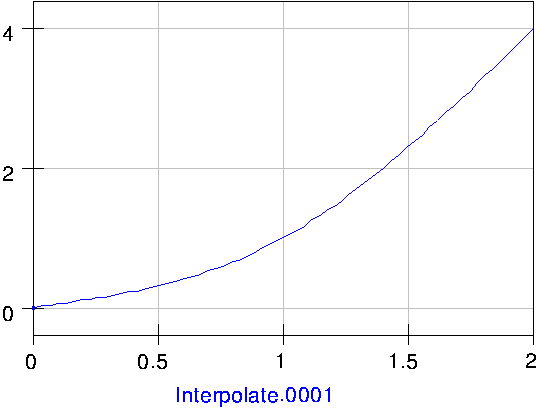
\includegraphics[%
  width=.5\linewidth]{interpolate_example}\end{center}


\caption{Interpolated curve}
\end{figure}


Use the Cartesian diagram to display it.

\begin{description}
\item [See~also]~
\end{description}
\textcolor{blue}{\hyperlink{sum}{sum()}}\textcolor{black}{,} \textcolor{blue}{\hyperlink{prod}{prod()}}


\newpage
\subsubsection*{\hypertarget{prod}{}{\Large prod\index{prod}()}}


\paragraph{\label{par:Prod}Product of vector elements.}

\begin{description}
\item [Syntax]~
\end{description}
y=prod(x)

\begin{description}
\item [Arguments]~
\end{description}
\begin{tabular}{|c|c|c|c|}
\hline 
Name&
Type&
Def. Range&
Required\tabularnewline
\hline
\hline 
x&
$\mathbb{R}$, $\mathbb{C}$, $\mathbb{R}^{n}$, $\mathbb{C}^{n}$&
$\left]-\infty,+\infty\right[$&
$\surd$\tabularnewline
\hline
\end{tabular}

\begin{description}
\item [Description]~
\end{description}
This function returns the product of the elements of a real or complex
vector.

\medskip{}
For $x\in$$\mathbb{C}^{n}$: $y=$$\prod\limits _{i=1}^{n}x_{i}$
\medskip{}

For \textit{x} being a real or complex number, \textit{x} itself is
returned.

\begin{description}
\item [Example]~
\end{description}
\begin{lyxlist}{00.00.0000}
\item [\texttt{y=prod(linspace(1,3,10))}]returns 583.
\end{lyxlist}
\begin{description}
\item [See~also]~
\end{description}
\textcolor{blue}{\hyperlink{sum}{sum()}}\textcolor{black}{,} \textcolor{blue}{\hyperlink{avg}{avg()}}\textcolor{black}{,}
\textcolor{blue}{\hyperlink{max}{max()}}\textcolor{black}{,} \textcolor{blue}{\hyperlink{min}{min()}}


\newpage
\subsubsection*{\hypertarget{sum}{}{\Large sum\index{sum}()}}


\paragraph{\label{par:Sum}Sum of vector elements.}

\begin{description}
\item [Syntax]~
\end{description}
y=sum(x)

\begin{description}
\item [Arguments]~
\end{description}
\begin{tabular}{|c|c|c|c|}
\hline 
Name&
Type&
Def. Range&
Required\tabularnewline
\hline
\hline 
x&
$\mathbb{R}$, $\mathbb{C}$, $\mathbb{R}^{n}$, $\mathbb{C}^{n}$&
$\left]-\infty,+\infty\right[$&
$\surd$\tabularnewline
\hline
\end{tabular}

\begin{description}
\item [Description]~
\end{description}
This function returns the sum of the elements of a real or complex
vector.

\medskip{}
For $x\in$$\mathbb{C}^{n}$: $y=$$\sum\limits _{i=1}^{n}x_{i}$
\medskip{}

For \textit{x} being a real or complex number, \textit{x} itself is
returned.

\begin{description}
\item [Example]~
\end{description}
\begin{lyxlist}{00.00.0000}
\item [\texttt{y=sum(linspace(1,3,10))}]returns 20.
\end{lyxlist}
\begin{description}
\item [See~also]~
\end{description}
\textcolor{blue}{\hyperlink{prod}{prod()}}\textcolor{black}{,} \textcolor{blue}{\hyperlink{avg}{avg()}}\textcolor{black}{,}
\textcolor{blue}{\hyperlink{max}{max()}}\textcolor{black}{,} \textcolor{blue}{\hyperlink{min}{min()}}


\newpage
\subsubsection*{\hypertarget{xvalue}{}{\Large xvalue\index{xvalue}()}}


\paragraph{\label{par:xvalue}Returns x-value which is associated with the y-value
nearest to a specified y-value in a given vector.}

\begin{description}
\item [Syntax]~
\end{description}
x=xvalue(f,yval)

\begin{description}
\item [Arguments]~
\end{description}
\begin{tabular}{|c|c|c|c|}
\hline 
Name&
Type&
Def. Range&
Required\tabularnewline
\hline
\hline 
f&
$\mathbb{R}^{n}$, $\mathbb{C}^{n}$&
$\left]-\infty,+\infty\right[$&
$\surd$\tabularnewline
\hline
yval&
$\mathbb{R}$, $\mathbb{C}$&
$\left]-\infty,+\infty\right[$&
$\surd$\tabularnewline
\hline
\end{tabular}

\begin{description}
\item [Description]~
\end{description}
This function returns the \textit{x}-value which is associated with
the \textit{y}-value nearest to \textit{yval} in the given vector
\textit{f}; therefore the vector \textit{f} must have a single data
dependency.

\begin{description}
\item [Example]~
\end{description}
\begin{lyxlist}{00.00.0000}
\item [\texttt{x=xvalue(f,1)}.]~
\end{lyxlist}
\begin{description}
\item [See~also]~
\end{description}
\textcolor{blue}{\hyperlink{yvalue}{yvalue()}}\textcolor{black}{,}
\textcolor{blue}{\hyperlink{interpolate}{interpolate()}}


\newpage
\subsubsection*{\hypertarget{yvalue}{}{\Large yvalue\index{yvalue}()}}


\paragraph{\label{par:yvalue}Returns y-value of a given vector which is located
nearest to the specified x-value.}

\begin{description}
\item [Syntax]~
\end{description}
y=yvalue(f,xval)

\begin{description}
\item [Arguments]~
\end{description}
\begin{tabular}{|c|c|c|c|}
\hline 
Name&
Type&
Def. Range&
Required\tabularnewline
\hline
\hline 
f&
$\mathbb{R}^{n}$, $\mathbb{C}^{n}$&
$\left]-\infty,+\infty\right[$&
$\surd$\tabularnewline
\hline
xval&
$\mathbb{R}$, $\mathbb{C}$&
$\left]-\infty,+\infty\right[$&
$\surd$\tabularnewline
\hline
\end{tabular}

\begin{description}
\item [Description]~
\end{description}
This function returns the y-value of the given vector \textit{f} which
is located nearest to the x-value \textit{xval}; therefore the vector
\textit{f} must have a single data dependency.

\begin{description}
\item [Example]~
\end{description}
\begin{lyxlist}{00.00.0000}
\item [\texttt{y=yvalue(f,1)}.]~
\end{lyxlist}
\begin{description}
\item [See~also]~
\end{description}
\textcolor{blue}{\hyperlink{xvalue}{xvalue()}}\textcolor{black}{,}
\textcolor{blue}{\hyperlink{interpolate}{interpolate()}}


\newpage
\tutsubsubsection{\label{sub:Differentiation-and-Integration}Differentiation and Integration}


\subsubsection*{\hypertarget{diff}{}{\Large diff\index{diff}()}}


\paragraph{\label{par:Differentiate}Differentiate vector with respect to another
vector.}

\begin{description}
\item [Syntax]~
\end{description}
z=diff(y,x,n)

\begin{description}
\item [Arguments]~
\end{description}
\begin{tabular}{|c|c|c|c|c|}
\hline 
Name&
Type&
Def. Range&
Required&
Default\tabularnewline
\hline
\hline 
y&
$\mathbb{R}^{k}$, $\mathbb{C}^{k}$&
$\left]-\infty,+\infty\right[$&
$\surd$&
\tabularnewline
\hline 
x&
$\mathbb{R}^{m}$, $\mathbb{C}^{m}$&
$\left]-\infty,+\infty\right[$&
$\surd$&
\tabularnewline
\hline 
n&
$\mathbb{N}$&
&
&
1\tabularnewline
\hline
\end{tabular}

\begin{description}
\item [Description]~
\end{description}
This function numerically differentiates a vector \textit{y} with
respect to a vector \textit{x}. If the optional integer parameter
\textit{n} is given, the n-th derivative is calculated. Differentiation
is executed for \textit{N=}min\textit{(k,m)} elements. For n=1,

\medskip{}
${\displaystyle \frac{\Delta y_{i}}{\Delta x_{i}}}=$$\left\{ \begin{array}{cc}
{\displaystyle \frac{1}{2}\left(\frac{y_{i}-y_{i-1}}{x_{i}-x_{i-1}}+\frac{y_{i+1}-y_{i}}{x_{i+1}-x_{i}}\right)} & \textrm{for}\: N-1>i>0\\
{\displaystyle \frac{y_{i+1}-y_{i}}{x_{i+1}-x_{i}}} & \textrm{for}\: i=0\\
{\displaystyle \frac{y_{i}-y_{i-1}}{x_{i}-x_{i-1}}} & \textrm{for}\: i=N-1\end{array}\right.$
\medskip{}

\noindent If \textit{n>1}, the result of the differentiation above
is assigned to \textit{y} and the aforementioned differentiation step
is repeated until the number of those steps is equal to \textit{n}.

\begin{description}
\item [Example]~
\end{description}
\begin{lyxlist}{00.00.0000}
\item [\texttt{z=diff(linspace(1,3,3),linspace(2,3,3))}]returns 2, 2, 2.
\end{lyxlist}
\begin{description}
\item [See~also]~
\end{description}
\textcolor{blue}{\hyperlink{integrate}{integrate()}}\textcolor{black}{,}
\textcolor{blue}{\hyperlink{sum}{sum()}}\textcolor{black}{,} \textcolor{blue}{\hyperlink{max}{max()}}\textcolor{black}{,}
\textcolor{blue}{\hyperlink{min}{min()}}


\newpage
\subsubsection*{\hypertarget{integrate}{}{\Large integrate\index{integrate}()}}


\paragraph{\label{par:Integrate}Integrate vector.}

\begin{description}
\item [Syntax]~
\end{description}
z=integrate(y,h)

\begin{description}
\item [Arguments]~
\end{description}
\begin{tabular}{|c|c|c|c|}
\hline 
Name&
Type&
Def. Range&
Required\tabularnewline
\hline
\hline 
y&
$\mathbb{R}$, $\mathbb{C}$, $\mathbb{R}^{n}$, $\mathbb{C}^{n}$&
$\left]-\infty,+\infty\right[$&
$\surd$\tabularnewline
\hline 
h&
$\mathbb{R}$, $\mathbb{C}$&
$\left]-\infty,+\infty\right[$&
$\surd$\tabularnewline
\hline
\end{tabular}

\begin{description}
\item [Description]~
\end{description}
This function numerically integrates a vector \textit{x} with respect
to a differential \textit{h}. The integration method is according
to the trapez rule:

\medskip{}
$\int f\left(t\right)dt\approx h\,\left({\displaystyle \frac{y_{0}}{2}}+y_{1}+y_{2}+\ldots+y_{n-1}+{\displaystyle \frac{y_{n}}{2}}\right)$
\medskip{}

\begin{description}
\item [Example]~
\end{description}
\noindent Calculate an approximation of the integral $\int\limits _{1}^{3}t\, dt$
using 105 points:

\begin{lyxlist}{00.00.0000}
\item [\texttt{z=integrate(linspace(1,3,105){*}linspace(1,3,105),0.02)}]returns
4.
\end{lyxlist}
\begin{description}
\item [See~also]~
\end{description}
\textcolor{blue}{\hyperlink{diff}{diff()}}\textcolor{black}{,} \textcolor{blue}{\hyperlink{sum}{sum()}}\textcolor{black}{,}
\textcolor{blue}{\hyperlink{max}{max()}}\textcolor{black}{,} \textcolor{blue}{\hyperlink{min}{min()}}


\newpage
\tutsubsubsection{\label{sub:Signal-Processing}Signal Processing}


\subsubsection*{\hypertarget{dft}{}{\Large dft\index{dft}()}}


\paragraph{\label{par:Discrete-Fourier-Transform}Discrete Fourier Transform.}

\begin{description}
\item [Syntax]~
\end{description}
y=dft(v,t)

\begin{description}
\item [Arguments]~
\end{description}
\begin{tabular}{|c|c|c|c|}
\hline 
Name&
Type&
Def. Range&
Required\tabularnewline
\hline
\hline 
v&
$\mathbb{R}^{n}$, $\mathbb{C}^{n}$&
$\left]-\infty,+\infty\right[$&
$\surd$\tabularnewline
\hline 
t&
$\mathbb{R}^{k}$, $\mathbb{C}^{k}$&
$\left]-\infty,+\infty\right[$&
$\surd$\tabularnewline
\hline
\end{tabular}

\begin{description}
\item [Description]~
\end{description}
This function computes the Discrete Fourier Transform (DFT) of a vector
\textit{v} with respect to a time vector \textit{t}. The advantage
of this function compared to \textcolor{blue}{\hyperlink{fft}{fft()}}
\textcolor{black}{is that} the number \textit{n} of components of
\textit{v} is arbitrary, while for the latter \textit{n} must be a
power of 2. The drawbacks are that dft() is slower and less accurate
than \textcolor{blue}{\hyperlink{fft}{fft()}}.

\begin{description}
\item [Example]~
\end{description}
This calculates the spectrum y(f) of a DC signal:

\begin{lyxlist}{00.00.0000}
\item [\texttt{y=dft(linspace(1,1,7),linspace(0,1,2))}]returns \begin{tabular}{|c|c|}
\hline 
Frequency&
y\tabularnewline
\hline
\hline 
0&
1\tabularnewline
\hline 
0.167&
-1.59e-17+j1.59e-17\tabularnewline
\hline 
$\vdots$&
$\vdots$\tabularnewline
\hline 
1&
2.22e-16-j1.11e-16\tabularnewline
\hline
\end{tabular}
\end{lyxlist}
Please note that in this example 7 points are used for the time vector
v. Since 7 is not a power of 2, the same expression used together
with the fft() function would lead to wrong results. Note also the
rounding errors at t>0, where {}``0'' would be the correct value.

\begin{description}
\item [See~also]~
\end{description}
\textcolor{blue}{\hyperlink{idft}{idft()}}\textcolor{black}{,} \textcolor{blue}{\hyperlink{fft}{fft()}}\textcolor{black}{,}
\textcolor{blue}{\hyperlink{ifft}{ifft()}}


\newpage
\subsubsection*{\hypertarget{fft}{}{\Large fft\index{fft}()}}


\paragraph{\label{par:Fast-Fourier-Transform}Fast Fourier Transform.}

\begin{description}
\item [Syntax]~
\end{description}
y=fft(v,t)

\begin{description}
\item [Arguments]~
\end{description}
\begin{tabular}{|c|c|c|c|}
\hline 
Name&
Type&
Def. Range&
Required\tabularnewline
\hline
\hline 
v&
$\mathbb{R}^{n}$, $\mathbb{C}^{n}$&
$\left]-\infty,+\infty\right[$&
$\surd$\tabularnewline
\hline 
t&
$\mathbb{R}^{k}$, $\mathbb{C}^{k}$&
$\left]-\infty,+\infty\right[$&
$\surd$\tabularnewline
\hline
\end{tabular}

\begin{description}
\item [Description]~
\end{description}
This function computes the Fast Fourier Transform (FFT) of a vector
\textit{v} with respect to a time vector \textit{t}. The number \textit{n}
of components of \textit{v} must be a power of 2.

\begin{description}
\item [Example]~
\end{description}
This calculates the spectrum y(f) of a DC signal:

\begin{lyxlist}{00.00.0000}
\item [\texttt{y=fft(linspace(1,1,8),linspace(0,1,2))}]returns \begin{tabular}{|c|c|}
\hline 
Frequency&
y\tabularnewline
\hline
\hline 
0&
1\tabularnewline
\hline 
0.143&
0\tabularnewline
\hline 
$\vdots$&
$\vdots$\tabularnewline
\hline 
1&
0\tabularnewline
\hline
\end{tabular}
\end{lyxlist}
\begin{description}
\item [See~also]~
\end{description}
\textcolor{blue}{\hyperlink{ifft}{ifft()}}\textcolor{black}{,} \textcolor{blue}{\hyperlink{dft}{dft()}}\textcolor{black}{,}
\textcolor{blue}{\hyperlink{idft}{idft()}}


\newpage
\subsubsection*{\hypertarget{idft}{}{\Large idft\index{idft}()}}


\paragraph{\label{par:Inverse-Discrete-Fourier}Inverse Discrete Fourier Transform.}

\begin{description}
\item [Syntax]~
\end{description}
y=idft(v,f)

\begin{description}
\item [Arguments]~
\end{description}
\begin{tabular}{|c|c|c|c|}
\hline 
Name&
Type&
Def. Range&
Required\tabularnewline
\hline
\hline 
v&
$\mathbb{R}^{n}$, $\mathbb{C}^{n}$&
$\left]-\infty,+\infty\right[$&
$\surd$\tabularnewline
\hline 
f&
$\mathbb{R}^{k}$, $\mathbb{C}^{k}$&
$\left]-\infty,+\infty\right[$&
$\surd$\tabularnewline
\hline
\end{tabular}

\begin{description}
\item [Description]~
\end{description}
This function computes the Inverse Discrete Fourier Transform (IDFT)
of a vector \textit{v} with respect to a frequency vector \textit{f}.
The advantage of this function compared to \textcolor{blue}{\hyperlink{ifft}{ifft()}}
\textcolor{black}{is that} the number \textit{n} of components of
\textit{v} is arbitrary, while for the latter \textit{n} must be a
power of 2. The drawbacks are that idft() is slower and less accurate
than \textcolor{blue}{\hyperlink{ifft}{ifft()}}.

\begin{description}
\item [Example]~
\end{description}
This calculates the time function y(t) belonging to a white spectrum:

\begin{lyxlist}{00.00.0000}
\item [\texttt{y=idft(linspace(1,1,7),linspace(0,1,2))}]returns \begin{tabular}{|c|c|}
\hline 
Frequency&
y\tabularnewline
\hline
\hline 
0&
7\tabularnewline
\hline 
0.167&
-1.11e-16-j1.11e-16\tabularnewline
\hline 
$\vdots$&
$\vdots$\tabularnewline
\hline 
1&
1.55e-15+j7.77e-16\tabularnewline
\hline
\end{tabular}
\end{lyxlist}
Please note that in this example 7 points are used for the spectrum
vector v. Since 7 is not a power of 2, the same expression used together
with the ifft() function would lead to wrong results. Note also the
rounding errors at t>0, where {}``0'' would be the correct value.

\begin{description}
\item [See~also]~
\end{description}
\textcolor{blue}{\hyperlink{dft}{dft()}}\textcolor{black}{,} \textcolor{blue}{\hyperlink{ifft}{ifft()}}\textcolor{black}{,}
\textcolor{blue}{\hyperlink{fft}{fft()}}


\newpage
\subsubsection*{\hypertarget{ifft}{}{\Large ifft\index{ifft}()}}


\paragraph{\label{par:Inverse-Fast-Fourier}Inverse Fast Fourier Transform.}

\begin{description}
\item [Syntax]~
\end{description}
y=ifft(v,f)

\begin{description}
\item [Arguments]~
\end{description}
\begin{tabular}{|c|c|c|c|}
\hline 
Name&
Type&
Def. Range&
Required\tabularnewline
\hline
\hline 
v&
$\mathbb{R}^{n}$, $\mathbb{C}^{n}$&
$\left]-\infty,+\infty\right[$&
$\surd$\tabularnewline
\hline 
f&
$\mathbb{R}^{k}$, $\mathbb{C}^{k}$&
$\left]-\infty,+\infty\right[$&
$\surd$\tabularnewline
\hline
\end{tabular}

\begin{description}
\item [Description]~
\end{description}
This function computes the Inverse Fast Fourier Transform (IFFT) of
a vector \textit{v} with respect to a frequency vector \textit{f}.
The number \textit{n} of components of \textit{v} must be a power
of 2.

\begin{description}
\item [Example]~
\end{description}
This calculates the time function y(t) belonging to a white spectrum:

\begin{lyxlist}{00.00.0000}
\item [\texttt{y=ifft(linspace(1,1,8),linspace(0,1,2))}]returns \begin{tabular}{|c|c|}
\hline 
Frequency&
y\tabularnewline
\hline
\hline 
0&
8\tabularnewline
\hline 
0.143&
0\tabularnewline
\hline 
$\vdots$&
$\vdots$\tabularnewline
\hline 
1&
0\tabularnewline
\hline
\end{tabular}
\end{lyxlist}
\begin{description}
\item [See~also]~
\end{description}
\textcolor{blue}{\hyperlink{fft}{fft()}}\textcolor{black}{,} \textcolor{blue}{\hyperlink{dft}{dft()}}\textcolor{black}{,}
\textcolor{blue}{\hyperlink{idft}{idft()}}


\newpage
\subsubsection*{\hypertarget{kbd}{}{\Large kbd\index{kbd}()}}


\paragraph{\label{par:Kaiser-Bessel-window}Kaiser-Bessel derived window.}

\begin{description}
\item [Syntax]~
\end{description}
y=kbd(a,n)

\noindent y=kbd(a)

\begin{description}
\item [Arguments]~
\end{description}
\begin{tabular}{|c|c|c|c|c|}
\hline 
Name&
Type&
Def. Range&
Required&
Default\tabularnewline
\hline
\hline 
a&
$\mathbb{R}$&
$\left]-\infty,+\infty\right[$&
$\surd$&
\tabularnewline
\hline 
n&
$\mathbb{N}$&
$\left[1,+\infty\right[$&
&
64\tabularnewline
\hline
\end{tabular}

\begin{description}
\item [Description]~
\end{description}
This function generates a Kaiser-Bessel window according to

\medskip{}
$y_{k}\quad\,=\:{\displaystyle \sqrt{\frac{\sum\limits _{i=0}^{k}I_{0}\left(\pi\, a\,\sqrt{1-\left(\frac{4\, i}{n}-1\right)}\right)}{\sum\limits _{i=0}^{\frac{n}{2}}I_{0}\left(\pi\, a\,\sqrt{1-\left(\frac{4\, i}{n}-1\right)}\right)}}}$,
\medskip{}

$y_{n-k-1}=\: y_{k}$
\medskip{}

for $0\leq k<\frac{n}{2}$
\medskip{}

\noindent If the parameter \textit{n} is not specified, \textit{n}=64
is assumed.

\begin{description}
\item [Example]~
\end{description}
\begin{lyxlist}{00.00.0000}
\item [\texttt{y=kbd(0.1,4)}]returns .
\end{lyxlist}
\begin{description}
\item [See~also]~
\end{description}
\textcolor{blue}{\hyperlink{dft}{dft()}}\textcolor{black}{,} \textcolor{blue}{\hyperlink{ifft}{ifft()}}\textcolor{black}{,}
\textcolor{blue}{\hyperlink{fft}{fft()}}


\tutsection{\label{chapter:electronics}Electronics Functions}
\tutsubsection{\label{sec:Unit-Conversion}Unit Conversion}

\subsubsection*{\hypertarget{dB}{}{\Large dB\index{dB}()}}

\paragraph{\label{par:dB}dB value.}

\begin{description}
\item [Syntax]~
\end{description}
y=dB(x)

\begin{description}
\item [Arguments]~
\end{description}
\begin{tabular}{|c|c|c|c|}
\hline 
Name&
Type&
Def. Range&
Required\tabularnewline
\hline
\hline 
x&
$\mathbb{R}$, $\mathbb{C}$, $\mathbb{R}^{n}$, $\mathbb{C}^{n}$&
$\left]-\infty,+\infty\right[$&
$\surd$\tabularnewline
\hline
\end{tabular}

\begin{description}
\item [Description]~
\end{description}
This function returns the dB value of a real or complex number or
vector.

\medskip{}
$y=20\,\log\left|x\right|$
\medskip{}

\noindent For \textit{x} being a vector the equation above is applied
to the components of \textit{x}.

\begin{description}
\item [Example]~
\end{description}
\begin{lyxlist}{00.00.0000}
\item [\texttt{y=db(10)}]returns 20.
\end{lyxlist}
\begin{description}
\item [See~also]~
\end{description}
\textcolor{blue}{\hyperlink{log10}{log10()}}


\newpage
\subsubsection*{\hypertarget{dbm}{}{\Large dbm\index{dbm}()}}


\paragraph{\label{par:dbm}Convert voltage to power in dBm.}

\begin{description}
\item [Syntax]~
\end{description}
y=dBm(u,Z0)

\noindent y=dBm(u)

\begin{description}
\item [Arguments]~
\end{description}
\begin{tabular}{|c|c|c|c|c|}
\hline 
Name&
Type&
Def. Range&
Required&
Default\tabularnewline
\hline
\hline 
u&
$\mathbb{R}$, $\mathbb{C}$, $\mathbb{R}^{n}$, $\mathbb{C}^{n}$&
$\left]-\infty,+\infty\right[$&
$\surd$&
\tabularnewline
\hline 
Z0&
$\mathbb{R}$, $\mathbb{C}$, $\mathbb{R}^{n}$, $\mathbb{C}^{n}$&
$\left]-\infty,+\infty\right[$&
&
50\tabularnewline
\hline
\end{tabular}

\begin{description}
\item [Description]~
\end{description}
This function returns the corresponding dBm power of a real or complex
voltage or vector \textit{u}. The impedance \textit{Z0} referred to
is either specified or 50$\Omega$.

\medskip{}
$y=10\,\log{\displaystyle \frac{\left|u\right|^{2}}{Z_{0}\,0.001W}}$
\medskip{}

\noindent For \textit{u} being a vector the equation above is applied
to the components of u.

\noindent Please note that \textit{u} is considered as a rms value,
not as an amplitude.

\begin{description}
\item [Example]~
\end{description}
\begin{lyxlist}{00.00.0000}
\item [\texttt{y=dbm(1)}]returns 13.
\end{lyxlist}
\begin{description}
\item [See~also]~
\end{description}
\textcolor{blue}{\hyperlink{dbm2w}{dbm2w()}}\textcolor{black}{,}
\textcolor{blue}{\hyperlink{w2dbm}{w2dbm()}}\textcolor{black}{,}
\textcolor{blue}{\hyperlink{log10}{log10()}}


\newpage
\subsubsection*{\hypertarget{dbm2w}{}{\Large dbm2w\index{dbm2w}()}}


\paragraph{\label{par:dbm2w}Convert power in dBm to power in Watts.}

\begin{description}
\item [Syntax]~
\end{description}
y=dBm2w(x)

\begin{description}
\item [Arguments]~
\end{description}
\begin{tabular}{|c|c|c|c|}
\hline 
Name&
Type&
Def. Range&
Required\tabularnewline
\hline
\hline 
x&
$\mathbb{R}$, $\mathbb{C}$, $\mathbb{R}^{n}$, $\mathbb{C}^{n}$&
$\left]-\infty,+\infty\right[$&
$\surd$\tabularnewline
\hline
\end{tabular}

\begin{description}
\item [Description]~
\end{description}
This function converts the real or complex power or power vector,
given in dBm, to the corresponding power in Watts.

\medskip{}
$y=0.001\,{\displaystyle 10^{\frac{x}{10}}}$
\medskip{}

\noindent For \textit{x} being a vector the equation above is applied
to the components of \textit{x}.

\begin{description}
\item [Example]~
\end{description}
\begin{lyxlist}{00.00.0000}
\item [\texttt{y=dbm2w(10)}]returns 0.01.
\end{lyxlist}
\begin{description}
\item [See~also]~
\end{description}
\textcolor{blue}{\hyperlink{dbm}{dbm()}}\textcolor{black}{,} \textcolor{blue}{\hyperlink{w2dbm}{w2dbm()}}


\newpage
\subsubsection*{\hypertarget{w2dbm}{}{\Large w2dbm\index{w2dbm}()}}


\paragraph{\label{par:w2dbm}Convert power in Watts to power in dBm.}

\begin{description}
\item [Syntax]~
\end{description}
y=w2dBm(x)

\begin{description}
\item [Arguments]~
\end{description}
\begin{tabular}{|c|c|c|c|}
\hline 
Name&
Type&
Def. Range&
Required\tabularnewline
\hline
\hline 
x&
$\mathbb{R}$, $\mathbb{C}$, $\mathbb{R}^{n}$, $\mathbb{C}^{n}$&
$\left]-\infty,+\infty\right[$&
$\surd$\tabularnewline
\hline
\end{tabular}

\begin{description}
\item [Description]~
\end{description}
This function converts the real or complex power or power vector,
given in Watts, to the corresponding power in dBm.

\medskip{}
$y=10\,\log{\displaystyle \frac{x}{0.001W}}$
\medskip{}

\noindent For \textit{x} being a vector the equation above is applied
to the components of \textit{x}.

\begin{description}
\item [Example]~
\end{description}
\begin{lyxlist}{00.00.0000}
\item [\texttt{y=w2dbm(1)}]returns 30.
\end{lyxlist}
\begin{description}
\item [See~also]~
\end{description}
\textcolor{blue}{\hyperlink{dbm}{dbm()}}\textcolor{black}{,} \textcolor{blue}{\hyperlink{dbm2w}{dbm2w()}}\textcolor{black}{,}
\textcolor{blue}{\hyperlink{log10}{log10()}}


\newpage
\tutsubsection{\label{sec:Reflection-Coefficients-and}Reflection Coefficients and
VSWR}


\subsubsection*{\hypertarget{rtoswr}{}{\Large rtoswr\index{rtoswr}()}}


\paragraph{\label{par:rtoswr}Converts reflection coefficient to voltage standing
wave ratio (VSWR).}

\begin{description}
\item [Syntax]~
\end{description}
s=rtoswr(r)

\begin{description}
\item [Arguments]~
\end{description}
\begin{tabular}{|c|c|c|c|}
\hline 
Name&
Type&
Def. Range&
Required\tabularnewline
\hline
\hline 
r&
$\mathbb{R}$, $\mathbb{C}$, $\mathbb{R}^{n}$, $\mathbb{C}^{n}$&
$\left|r\right|\leq1$&
$\surd$\tabularnewline
\hline
\end{tabular}

\begin{description}
\item [Description]~
\end{description}
For a real or complex reflection coefficient \textit{r}, this function
calculates the corresponding voltage standing wave ratio (VSWR) \textit{s}
according to 

\medskip{}
$s={\displaystyle \frac{1+\left|r\right|}{1-\left|r\right|}}$
\medskip{}

\noindent VSWR is a real number and if usually given in the notation
{}``s : 1''.

\noindent For \textit{r} being a vector the equation above is applied
to the components of \textit{r}.

\begin{description}
\item [Examples]~
\end{description}
\texttt{s=rtoswr(0)} returns 1.

\begin{lyxlist}{00.00.0000}
\item [\texttt{s=rtoswr(0.1+0.2{*}i)}]returns 1.58.
\end{lyxlist}
\begin{description}
\item [See~also]~
\end{description}
\textcolor{blue}{\hyperlink{ytor}{ytor()}}\textcolor{black}{,} \textcolor{blue}{\hyperlink{ztor}{ztor()}}\textcolor{black}{,}
\textcolor{blue}{\hyperlink{rtoy}{rtoy()}}\textcolor{black}{,} \textcolor{blue}{\hyperlink{rtoz}{rtoz()}}


\newpage
\subsubsection*{\hypertarget{rtoy}{}{\Large rtoy\index{rtoy}()}}


\paragraph{\label{par:rtoy}Converts reflection coefficient to admittance.}

\begin{description}
\item [Syntax]~
\end{description}
y=rtoy(r)

\noindent y=rtoy(r, Z0)

\begin{description}
\item [Arguments]~
\end{description}
\begin{tabular}{|c|c|c|c|c|}
\hline 
Name&
Type&
Def. Range&
Required&
Default\tabularnewline
\hline
\hline 
r&
$\mathbb{R}$, $\mathbb{C}$, $\mathbb{R}^{n}$, $\mathbb{C}^{n}$&
$\left|r\right|\leq1$&
$\surd$&
\tabularnewline
\hline
Z0&
$\mathbb{R}$, $\mathbb{C}$&
$\left]-\infty,+\infty\right[$&
&
50\tabularnewline
\hline
\end{tabular}

\begin{description}
\item [Description]~
\end{description}
For a real or complex reflection coefficient \textit{r}, this function
calculates the corresponding admittance \textit{y} according to 

\medskip{}
$y={\displaystyle \frac{1}{Z_{0}}\,\frac{1-r}{1+r}}$
\medskip{}

\noindent If the reference impedance \textit{Z0} is not provided,
the function assumes \textit{Z0} = 50$\Omega$.

\noindent For \textit{r} being a vector the equation above is applied
to the components of \textit{r}.

\begin{description}
\item [Example]~
\end{description}
\begin{lyxlist}{00.00.0000}
\item [\texttt{y=rtoy(0.333)}]returns 0.01.
\end{lyxlist}
\begin{description}
\item [See~also]~
\end{description}
\textcolor{blue}{\hyperlink{ytor}{ytor()}}\textcolor{black}{,} \textcolor{blue}{\hyperlink{ztor}{ztor()}}\textcolor{black}{,}
\textcolor{blue}{\hyperlink{rtoswr}{rtoswr()}}


\newpage
\subsubsection*{\hypertarget{rtoz}{}{\Large rtoz\index{rtoz}()}}


\paragraph{\label{par:rtoz}Converts reflection coefficient to impedance.}

\begin{description}
\item [Syntax]~
\end{description}
z=rtoz(r)

\noindent z=rtoz(r, Z0)

\begin{description}
\item [Arguments]~
\end{description}
\begin{tabular}{|c|c|c|c|c|}
\hline 
Name&
Type&
Def. Range&
Required&
Default\tabularnewline
\hline
\hline 
r&
$\mathbb{R}$, $\mathbb{C}$, $\mathbb{R}^{n}$, $\mathbb{C}^{n}$&
$\left|r\right|\leq1$&
$\surd$&
\tabularnewline
\hline
Z0&
$\mathbb{R}$, $\mathbb{C}$&
$\left]-\infty,+\infty\right[$&
&
50\tabularnewline
\hline
\end{tabular}

\begin{description}
\item [Description]~
\end{description}
For a real or complex reflection coefficient \textit{r}, this function
calculates the corresponding impedance \textit{Z} according to 

\medskip{}
$Z={\displaystyle Z_{0}\,\frac{1-r}{1+r}}$
\medskip{}

\noindent If the reference impedance \textit{Z0} is not provided,
the function assumes \textit{Z0} = 50$\Omega$.

\noindent For \textit{r} being a vector the equation above is applied
to the components of \textit{r}.

\begin{description}
\item [Example]~
\end{description}
\begin{lyxlist}{00.00.0000}
\item [\texttt{z=rtoz(0.333)}]returns 99.9.
\end{lyxlist}
\begin{description}
\item [See~also]~
\end{description}
\textcolor{blue}{\hyperlink{ztor}{ztor()}}\textcolor{black}{,} \textcolor{blue}{\hyperlink{ytor}{ytor()}}\textcolor{black}{,}
\textcolor{blue}{\hyperlink{rtoswr}{rtoswr()}}


\newpage
\subsubsection*{\hypertarget{ytor}{}{\Large ytor\index{ytor}()}}


\paragraph{\label{par:ytor}Converts admittance to reflection coefficient.}

\begin{description}
\item [Syntax]~
\end{description}
r=ytor(Y)

\noindent r=ytor(Y, Z0)

\begin{description}
\item [Arguments]~
\end{description}
\begin{tabular}{|c|c|c|c|c|}
\hline 
Name&
Type&
Def. Range&
Required&
Default\tabularnewline
\hline
\hline 
Y&
$\mathbb{R}$, $\mathbb{C}$, $\mathbb{R}^{n}$, $\mathbb{C}^{n}$&
$\left]-\infty,+\infty\right[$&
$\surd$&
\tabularnewline
\hline
Z0&
$\mathbb{R}$, $\mathbb{C}$&
$\left]-\infty,+\infty\right[$&
&
50\tabularnewline
\hline
\end{tabular}

\begin{description}
\item [Description]~
\end{description}
For a real or complex admittance \textit{y}, this function calculates
the corresponding reflection coefficient according to 

\medskip{}
$r={\displaystyle \frac{1-Y\, Z_{0}}{1+Y\, Z_{0}}}$
\medskip{}

\noindent For \textit{Y} being a vector the equation above is applied
to the components of \textit{Y}.

\noindent If the reference impedance \textit{Z0} is not provided,
the function assumes \textit{Z0} = 50$\Omega$.

\noindent Often a dB measure is given for the reflection coefficient,
the so called {}``return loss'':

$RL=-20\,\log\left|r\right|$ {[}dB{]}

\begin{description}
\item [Example]~
\end{description}
\begin{lyxlist}{00.00.0000}
\item [\texttt{r=ytor(0.01)}]returns 0.333.
\end{lyxlist}
\begin{description}
\item [See~also]~
\end{description}
\textcolor{blue}{\hyperlink{rtoy}{rtoy()}}\textcolor{black}{,} \textcolor{blue}{\hyperlink{rtoz}{rtoz()}}\textcolor{black}{,}
\textcolor{blue}{\hyperlink{rtoswr}{rtoswr()}}\textcolor{black}{,}
\textcolor{blue}{\hyperlink{log10}{log10()}}\textcolor{black}{,}
\textcolor{blue}{\hyperlink{dB}{dB()}}


\newpage
\subsubsection*{\hypertarget{ztor}{}{\Large ztor\index{ztor}()}}


\paragraph{\label{par:ztor}Converts impedance to reflection coefficient.}

\begin{description}
\item [Syntax]~
\end{description}
r=ztor(Z)

\noindent r=ztor(Z, Z0)

\begin{description}
\item [Arguments]~
\end{description}
\begin{tabular}{|c|c|c|c|c|}
\hline 
Name&
Type&
Def. Range&
Required&
Default\tabularnewline
\hline
\hline 
Z&
$\mathbb{R}$, $\mathbb{C}$, $\mathbb{R}^{n}$, $\mathbb{C}^{n}$&
$\left]-\infty,+\infty\right[$&
$\surd$&
\tabularnewline
\hline
Z0&
$\mathbb{R}$, $\mathbb{C}$&
$\left]-\infty,+\infty\right[$&
&
50\tabularnewline
\hline
\end{tabular}

\begin{description}
\item [Description]~
\end{description}
For a real or complex impedance \textit{Z}, this function calculates
the corresponding reflection coefficient according to 

\medskip{}
$r={\displaystyle \frac{Z-Z_{0}}{Z+Z_{0}}}$
\medskip{}

\noindent For \textit{Z} being a vector the equation above is applied
to the components of \textit{Z}.

\noindent If the reference impedance \textit{Z0} is not provided,
the function assumes \textit{Z0} = 50$\Omega$.

\noindent Often a dB measure is given for the reflection coefficient,
the so called {}``return loss'':

\noindent $RL=-20\,\log\left|r\right|$ {[}dB{]}

\begin{description}
\item [Example]~
\end{description}
\begin{lyxlist}{00.00.0000}
\item [\texttt{r=ztor(100)}]returns 0.333.
\end{lyxlist}
\begin{description}
\item [See~also]~
\end{description}
\textcolor{blue}{\hyperlink{rtoz}{rtoz()}}\textcolor{black}{,} \textcolor{blue}{\hyperlink{rtoy}{rtoy()}}\textcolor{black}{,}
\textcolor{blue}{\hyperlink{rtoswr}{rtoswr()}}\textcolor{black}{,}
\textcolor{blue}{\hyperlink{log10}{log10()}}\textcolor{black}{,}
\textcolor{blue}{\hyperlink{dB}{dB()}}


\newpage
\tutsubsection{\label{sec:N-Port-Matrix-Conversions}N-Port Matrix Conversions}


\subsubsection*{\hypertarget{stos}{}{\Large stos\index{stos}()}}


\paragraph{\label{par:stos}Converts S-parameter matrix to S-parameter matrix
with different reference impedance(s).}

\begin{description}
\item [Syntax]~
\end{description}
y=stos(S, Zref)

\noindent y=stos(S, Zref, Z0)

\begin{description}
\item [Arguments]~
\end{description}
\begin{tabular}{|c|c|c|c|c|}
\hline 
Name&
Type&
Def. Range&
Required&
Default\tabularnewline
\hline
\hline 
S&
$\mathbb{R}^{n\times n}$, $\mathbb{C}^{n\times n}$&
\begin{tabular}{l}
$\left|S_{ij}\right|\in\left]-\infty,+\infty\right[,\:1\leq i,j\leq n$\tabularnewline
$\left|S_{ii}\right|\leq1,\:1\leq i\leq n$\tabularnewline
\end{tabular}&
$\surd$&
\tabularnewline
\hline
Zref&
$\mathbb{R}$, $\mathbb{C}$, $\mathbb{R}^{n}$, $\mathbb{C}^{n}$&
$\left]-\infty,+\infty\right[$&
$\surd$&
\tabularnewline
\hline
Z0&
$\mathbb{R}$, $\mathbb{C}$, $\mathbb{R}^{n}$, $\mathbb{C}^{n}$&
$\left]-\infty,+\infty\right[$&
&
50\tabularnewline
\hline
\end{tabular}

\begin{description}
\item [Description]~
\end{description}
This function converts a real or complex scattering parameter matrix
\textit{S} into a scattering matrix \textit{Y}. \textit{S} has a reference
impedance \textit{Zref}, whereas the created scattering matrix \textit{Y}
has a reference impedance \textit{Z0}.

\noindent If the reference impedance \textit{Z0} is not provided,
the function assumes \textit{Z0} = 50$\Omega$.

\noindent Both \textit{Zref} and \textit{Z0} can be real or complex
numbers or vectors; in the latter case the function operates on the
elements of \textit{Zref} and \textit{Z0}.

\begin{description}
\item [Example]~
\end{description}
Conversion of 50$\Omega$ terminated S-parameters to 100$\Omega$
terminated S-parameters:

\begin{lyxlist}{00.00.0000}
\item [\texttt{S2=stos(eye(2){*}0.1,50,100)}]returns \begin{tabular}{|c|c|}
\hline 
-0.241&
0\tabularnewline
\hline
0&
-0.241\tabularnewline
\hline
\end{tabular}.
\end{lyxlist}
\begin{description}
\item [See~also]~
\end{description}
\textcolor{blue}{\hyperlink{twoport}{twoport()}}\textcolor{black}{,}
\textcolor{blue}{\hyperlink{stoy}{stoy()}}\textcolor{black}{,} \textcolor{blue}{\hyperlink{stoz}{stoz()}}


\newpage
\subsubsection*{\hypertarget{stoy}{}{\Large stoy\index{stoy}()}}


\paragraph{\label{par:stoy}Converts S-parameter matrix to Y-parameter matrix.}

\begin{description}
\item [Syntax]~
\end{description}
Y=stoy(S)

\noindent Y=stoy(S, Zref)

\begin{description}
\item [Arguments]~
\end{description}
\begin{tabular}{|c|c|c|c|c|}
\hline 
Name&
Type&
Def. Range&
Required&
Default\tabularnewline
\hline
\hline 
S&
$\mathbb{R}^{n\times n}$, $\mathbb{C}^{n\times n}$&
\begin{tabular}{l}
$\left|S_{ij}\right|\in\left]-\infty,+\infty\right[,\:1\leq i,j\leq n$\tabularnewline
$\left|S_{ii}\right|\leq1,\:1\leq i\leq n$\tabularnewline
\end{tabular}&
$\surd$&
\tabularnewline
\hline
Zref&
$\mathbb{R}$, $\mathbb{C}$, $\mathbb{R}^{n}$, $\mathbb{C}^{n}$&
$\left]-\infty,+\infty\right[$&
&
50\tabularnewline
\hline
\end{tabular}

\begin{description}
\item [Description]~
\end{description}
This function converts a real or complex scattering parameter matrix
\textit{S} into an admittance matrix \textit{Y}. \textit{S} has a
reference impedance \textit{Zref}, which is assumed to be \textit{Zref}
= 50$\Omega$ if not provided by the user.

\noindent \textit{Zref} can be real or complex number or vector; in
the latter case the function operates on the elements of \textit{Zref}.

\begin{description}
\item [Example]~
\end{description}
\begin{lyxlist}{00.00.0000}
\item [\texttt{Y=stoy(eye(2){*}0.1,100)}]returns \begin{tabular}{|c|c|}
\hline 
0.00818&
0\tabularnewline
\hline
0&
0.00818\tabularnewline
\hline
\end{tabular}.
\end{lyxlist}
\begin{description}
\item [See~also]~
\end{description}
\textcolor{blue}{\hyperlink{twoport}{twoport()}}\textcolor{black}{,}
\textcolor{blue}{\hyperlink{stos}{stos()}}\textcolor{black}{,} \textcolor{blue}{\hyperlink{stoz}{stoz()}}\textcolor{black}{,}
\textcolor{blue}{\hyperlink{ytos}{ytos()}}


\newpage
\subsubsection*{\hypertarget{stoz}{}{\Large stoz\index{stoz}()}}


\paragraph{\label{par:stoz}Converts S-parameter matrix to Z-parameter matrix.}

\begin{description}
\item [Syntax]~
\end{description}
Z=stoz(S)

\noindent Z=stoz(S, Zref)

\begin{description}
\item [Arguments]~
\end{description}
\begin{tabular}{|c|c|c|c|c|}
\hline 
Name&
Type&
Def. Range&
Required&
Default\tabularnewline
\hline
\hline 
S&
$\mathbb{R}^{n\times n}$, $\mathbb{C}^{n\times n}$&
\begin{tabular}{l}
$\left|S_{ij}\right|\in\left]-\infty,+\infty\right[,\:1\leq i,j\leq n$\tabularnewline
$\left|S_{ii}\right|\leq1,\:1\leq i\leq n$\tabularnewline
\end{tabular}&
$\surd$&
\tabularnewline
\hline
Zref&
$\mathbb{R}$, $\mathbb{C}$, $\mathbb{R}^{n}$, $\mathbb{C}^{n}$&
$\left]-\infty,+\infty\right[$&
&
50\tabularnewline
\hline
\end{tabular}

\begin{description}
\item [Description]~
\end{description}
This function converts a real or complex scattering parameter matrix
\textit{S} into an impedance matrix \textit{Z}. \textit{S} has a reference
impedance \textit{Zref}, which is assumed to be \textit{Zref} = 50$\Omega$
if not provided by the user.

\noindent \textit{Zref} can be real or complex number or vector; in
the latter case the function operates on the elements of \textit{Zref}.

\begin{description}
\item [Example]~
\end{description}
\begin{lyxlist}{00.00.0000}
\item [\texttt{Z=stoz(eye(2){*}0.1,100)}]returns \begin{tabular}{|c|c|}
\hline 
122&
0\tabularnewline
\hline
0&
122\tabularnewline
\hline
\end{tabular}.
\end{lyxlist}
\begin{description}
\item [See~also]~
\end{description}
\textcolor{blue}{\hyperlink{twoport}{twoport()}}\textcolor{black}{,}
\textcolor{blue}{\hyperlink{stos}{stos()}}\textcolor{black}{,} \textcolor{blue}{\hyperlink{stoy}{stoy()}}\textcolor{black}{,}
\textcolor{blue}{\hyperlink{ztos}{ztos()}}


\newpage
\subsubsection*{\hypertarget{twoport}{}{\Large twoport\index{twoport}()}}


\paragraph{\label{par:twoport}Converts a two-port matrix from one representation
into another.}

\begin{description}
\item [Syntax]~
\end{description}
U=twoport(X, from, to)

\begin{description}
\item [Arguments]~
\end{description}
\begin{tabular}{|c|c|c|c|}
\hline 
Name&
Type&
Def. Range&
Required\tabularnewline
\hline
\hline 
X&
$\mathbb{R}^{2\times2}$, $\mathbb{C}^{2\times2}$&
$\left]-\infty,+\infty\right[$&
$\surd$\tabularnewline
\hline
from&
Character&
$\left\{ ^{\prime}Y{}^{\prime},\,{}^{\prime}Z{}^{\prime},\,{}^{\prime}H{}^{\prime},\,{}^{\prime}G{}^{\prime},\,{}^{\prime}A{}^{\prime},\,{}^{\prime}S{}^{\prime},\,{}^{\prime}T{}^{\prime}\right\} $&
$\surd$\tabularnewline
\hline
to&
Character&
$\left\{ ^{\prime}Y{}^{\prime},\,{}^{\prime}Z{}^{\prime},\,{}^{\prime}H{}^{\prime},\,{}^{\prime}G{}^{\prime},\,{}^{\prime}A{}^{\prime},\,{}^{\prime}S{}^{\prime},\,{}^{\prime}T{}^{\prime}\right\} $&
$\surd$\tabularnewline
\hline
\end{tabular}

\begin{description}
\item [Description]~
\end{description}
This function converts a real or complex two-port matrix \textit{X}
from one representation into another. 

\begin{description}
\item [Example]~
\end{description}
Transfer a two-port Y matrix Y1 into a Z matrix:

\begin{lyxlist}{00.00.0000}
\item [\texttt{Y1=eye(2){*}0.1}]~
\item [\texttt{Z1=twoport(Y1,'Y','Z')}]returns \begin{tabular}{|c|c|}
\hline 
10&
0\tabularnewline
\hline
0&
10\tabularnewline
\hline
\end{tabular}.
\end{lyxlist}
\begin{description}
\item [See~also]~
\end{description}
\textcolor{blue}{\hyperlink{stos}{stos()}}\textcolor{black}{,} \textcolor{blue}{\hyperlink{ytos}{ytos()}}\textcolor{black}{,}
\textcolor{blue}{\hyperlink{ztos}{ztos()}}\textcolor{black}{,} \textcolor{blue}{\hyperlink{stoz}{stoz()}}\textcolor{black}{,}
\textcolor{blue}{\hyperlink{stoy}{stoy()}}\textcolor{black}{,} \textcolor{blue}{\hyperlink{ytoz}{ytoz()}}\textcolor{black}{,}
\textcolor{blue}{\hyperlink{ztoy}{ztoy()}}


\newpage
\subsubsection*{\hypertarget{ytos}{}{\Large ytos\index{ytos}()}}


\paragraph{\label{par:ytos}Converts Y-parameter matrix to S-parameter matrix.}

\begin{description}
\item [Syntax]~
\end{description}
S=ytos(Y)

\noindent S=ytos(Y, Z0)

\begin{description}
\item [Arguments]~
\end{description}
\begin{tabular}{|c|c|c|c|c|}
\hline 
Name&
Type&
Def. Range&
Required&
Default\tabularnewline
\hline
\hline 
Y&
$\mathbb{R}^{n\times n}$, $\mathbb{C}^{n\times n}$&
$\left]-\infty,+\infty\right[$&
$\surd$&
\tabularnewline
\hline
Z0&
$\mathbb{R}$, $\mathbb{C}$, $\mathbb{R}^{n}$, $\mathbb{C}^{n}$&
$\left]-\infty,+\infty\right[$&
&
50\tabularnewline
\hline
\end{tabular}

\begin{description}
\item [Description]~
\end{description}
This function converts a real or complex admittance matrix \textit{Y}
into a scattering parameter matrix \textit{S}. \textit{Y} has a reference
impedance \textit{Z0}, which is assumed to be \textit{Z0} = 50$\Omega$
if not provided by the user.

\noindent \textit{Z0} can be real or complex number or vector; in
the latter case the function operates on the elements of \textit{Z0}.

\begin{description}
\item [Example]~
\end{description}
\begin{lyxlist}{00.00.0000}
\item [\texttt{S=ytos(eye(2){*}0.1,100)}]returns \begin{tabular}{|c|c|}
\hline 
-0.818&
0\tabularnewline
\hline
0&
-0.818\tabularnewline
\hline
\end{tabular}.
\end{lyxlist}
\begin{description}
\item [See~also]~
\end{description}
\textcolor{blue}{\hyperlink{twoport}{twoport()}}\textcolor{black}{,}
\textcolor{blue}{\hyperlink{stos}{stos()}}\textcolor{black}{,} \textcolor{blue}{\hyperlink{ztos}{ztos()}}\textcolor{black}{,}
\textcolor{blue}{\hyperlink{stoy}{stoy()}}


\newpage
\subsubsection*{\hypertarget{ytoz}{}{\Large ytoz\index{ytoz}()}}


\paragraph{\label{par:ytoz}Converts Y-parameter matrix to Z-parameter matrix.}

\begin{description}
\item [Syntax]~
\end{description}
Z=ytoz(Y)

\begin{description}
\item [Arguments]~
\end{description}
\begin{tabular}{|c|c|c|c|}
\hline 
Name&
Type&
Def. Range&
Required\tabularnewline
\hline
\hline 
Y&
$\mathbb{R}^{n\times n}$, $\mathbb{C}^{n\times n}$&
$\left]-\infty,+\infty\right[$&
$\surd$\tabularnewline
\hline
\end{tabular}

\begin{description}
\item [Description]~
\end{description}
This function converts a real or complex admittance matrix \textit{Y}
into an impedance matrix \textit{Z}. 

\begin{description}
\item [Example]~
\end{description}
\begin{lyxlist}{00.00.0000}
\item [\texttt{Z=ytoz(eye(2){*}0.1)}]returns \begin{tabular}{|c|c|}
\hline 
10&
0\tabularnewline
\hline
0&
10\tabularnewline
\hline
\end{tabular}.
\end{lyxlist}
\begin{description}
\item [See~also]~
\end{description}
\textcolor{blue}{\hyperlink{twoport}{twoport()}}\textcolor{black}{,}
\textcolor{blue}{\hyperlink{ztoy}{ztoy()}}


\newpage
\subsubsection*{\hypertarget{ztos}{}{\Large ztos\index{ztos}()}}


\paragraph{\label{par:ztos}Converts Z-parameter matrix to S-parameter matrix.}

\begin{description}
\item [Syntax]~
\end{description}
S=ztos(Z)

\noindent S=ztos(Z, Z0)

\begin{description}
\item [Arguments]~
\end{description}
\begin{tabular}{|c|c|c|c|c|}
\hline 
Name&
Type&
Def. Range&
Required&
Default\tabularnewline
\hline
\hline 
Z&
$\mathbb{R}^{n\times n}$, $\mathbb{C}^{n\times n}$&
$\left]-\infty,+\infty\right[$&
$\surd$&
\tabularnewline
\hline
Z0&
$\mathbb{R}$, $\mathbb{C}$, $\mathbb{R}^{n}$, $\mathbb{C}^{n}$&
$\left]-\infty,+\infty\right[$&
&
50\tabularnewline
\hline
\end{tabular}

\begin{description}
\item [Description]~
\end{description}
This function converts a real or complex impedance matrix \textit{Z}
into a scattering parameter matrix \textit{S}. \textit{Z} has a reference
impedance \textit{Z0}, which is assumed to be \textit{Z0} = 50$\Omega$
if not provided by the user.

\noindent \textit{Z0} can be real or complex number or vector; in
the latter case the function operates on the elements of \textit{Z0}.

\begin{description}
\item [Example]~
\end{description}
\begin{lyxlist}{00.00.0000}
\item [\texttt{S=ztos(eye(2){*}0.1,100)}]returns \begin{tabular}{|c|c|}
\hline 
-0.998&
0\tabularnewline
\hline
0&
-0.998\tabularnewline
\hline
\end{tabular}.
\end{lyxlist}
\begin{description}
\item [See~also]~
\end{description}
\textcolor{blue}{\hyperlink{twoport}{twoport()}}\textcolor{black}{,}
\textcolor{blue}{\hyperlink{twoport}{twoport()}}\textcolor{black}{,}
\textcolor{blue}{\hyperlink{stos}{stos()}}\textcolor{black}{,} \textcolor{blue}{\hyperlink{ytos}{ytos()}}\textcolor{black}{,}
\textcolor{blue}{\hyperlink{stoz}{stoz()}}


\newpage
\subsubsection*{\hypertarget{ztoy}{}{\Large ztoy\index{ztoy}()}}


\paragraph{\label{par:ztoy}Converts Z-parameter matrix to Y-parameter matrix.}

\begin{description}
\item [Syntax]~
\end{description}
Y=ztoy(Z)

\begin{description}
\item [Arguments]~
\end{description}
\begin{tabular}{|c|c|c|c|}
\hline 
Name&
Type&
Def. Range&
Required\tabularnewline
\hline
\hline 
Z&
$\mathbb{R}^{n\times n}$, $\mathbb{C}^{n\times n}$&
$\left]-\infty,+\infty\right[$&
$\surd$\tabularnewline
\hline
\end{tabular}

\begin{description}
\item [Description]~
\end{description}
This function converts a real or complex impedance matrix \textit{Z}
into an admittance matrix \textit{Y}. 

\begin{description}
\item [Example]~
\end{description}
\begin{lyxlist}{00.00.0000}
\item [\texttt{Y=ztoy(eye(2){*}0.1)}]returns \begin{tabular}{|c|c|}
\hline 
10&
0\tabularnewline
\hline
0&
10\tabularnewline
\hline
\end{tabular}.
\end{lyxlist}
\begin{description}
\item [See~also]~
\end{description}
\textcolor{blue}{\hyperlink{twoport}{twoport()}}\textcolor{black}{,}
\textcolor{blue}{\hyperlink{ytoz}{ytoz()}}


\newpage
\tutsubsection{\label{sec:Amplifiers}Amplifiers}


\subsubsection*{\hypertarget{GaCircle}{}{\Large GaCircle\index{GaCircle}()}}


\paragraph{\label{par:GaCircle}Circle(s) with constant available power gain
Ga in the source plane.}

\begin{description}
\item [Syntax]~
\end{description}
y=GaCircle(X,Ga,v)

\noindent y=GaCircle(X,Ga,n)

\noindent y=GaCircle(X,Ga)

\begin{description}
\item [Arguments]~
\end{description}
\begin{tabular}{|c|c|c|c|c|}
\hline 
Name&
Type&
Def. Range&
Required&
Default\tabularnewline
\hline
\hline 
X&
$\mathbb{R}^{2\times2\times p}$, $\mathbb{C}^{2\times2\times p}$&
$\left]-\infty,+\infty\right[$&
$\surd$&
\tabularnewline
\hline
v&
$\mathbb{R}^{n}$&
$\left[0,360\right]^{o}$&
&
\tabularnewline
\hline
Ga&
$\mathbb{R}$, $\mathbb{R}^{m}$&
$\left[0,+\infty\right[$&
$\surd$&
\tabularnewline
\hline
n&
$\mathbb{N}$&
$\left[2,+\infty\right[$&
&
64\tabularnewline
\hline
\end{tabular}

\begin{description}
\item [Description]~
\end{description}
This function generates the points of the circle of constant available
power gain $G_{A}$ in the complex source plane ($r_{S}$) of an amplifier.
The amplifier is described by a two-port S-parameter matrix \textit{S}.
Radius \textit{r} and center \textit{c} of this circle are calculated
as follows:

\medskip{}
\noindent $r=\frac{{\displaystyle \sqrt{1-2\cdot K\cdot g_{A}\cdot\left|S_{12}S_{21}\right|+g_{A}^{2}\cdot\left|S_{12}S_{21}\right|^{2}}}}{{\displaystyle \left|1+g_{A}\cdot\left(\left|S_{11}\right|^{2}-\left|\Delta\right|^{2}\right)\right|}}$
and $c={\displaystyle \frac{g_{A}\left(S_{11}^{*}-S_{22}\,\Delta{}^{*}\right)}{1+g_{A}\left(\left|S_{11}\right|^{2}-\left|\Delta\right|^{2}\right)}}$,

\medskip{}
where $g_{A}={\displaystyle \frac{G_{A}}{\left|S_{21}\right|^{2}}}$
and $K$ Rollet stability factor. $\Delta$ denotes determinant of
$S$.
\medskip{}

\noindent The points of the circle can be specified by the angle vector
\textit{v}, where the angle must be given in degrees. Another possibility
is to specify the number \textit{n} of angular equally distributed
points around the circle. If no additional argument to \textit{X}
is given, 64 points are taken. The available power gain can also be
specified in a vector \textit{Ga}, leading to the generation of m
circles, where m is the size of \textit{Ga}.

\noindent Please also refer to {}``Qucs - Technical Papers'', chapter
1.5.

\begin{description}
\item [Example]~
\end{description}
\begin{lyxlist}{00.00.0000}
\item [\texttt{v=GaCircle(S)}]~
\end{lyxlist}
\begin{description}
\item [See~also]~
\end{description}
\textcolor{blue}{\hyperlink{GpCircle}{GpCircle()}}\textcolor{black}{,}
\textcolor{blue}{\hyperlink{Rollet}{Rollet()}}


\newpage
\subsubsection*{\hypertarget{GpCircle}{}{\Large GpCircle\index{GpCircle}()}}


\paragraph{\label{par:GpCircle}Circle(s) with constant operating power gain
Gp in the load plane.}

\begin{description}
\item [Syntax]~
\end{description}
y=GpCircle(X,Gp,v)

\noindent y=GpCircle(X,Gp,n)

\noindent y=GpCircle(X,Gp)

\begin{description}
\item [Arguments]~
\end{description}
\begin{tabular}{|c|c|c|c|c|}
\hline 
Name&
Type&
Def. Range&
Required&
Default\tabularnewline
\hline
\hline 
X&
$\mathbb{R}^{2\times2\times p}$, $\mathbb{C}^{2\times2\times p}$&
$\left]-\infty,+\infty\right[$&
$\surd$&
\tabularnewline
\hline
v&
$\mathbb{R}^{n}$ &
$\left[0,360\right]^{o}$&
&
\tabularnewline
\hline
Gp&
$\mathbb{R}$, $\mathbb{R}^{m}$&
$\left[0,+\infty\right[$&
$\surd$&
\tabularnewline
\hline
n&
$\mathbb{N}$&
$\left[2,+\infty\right[$&
&
64\tabularnewline
\hline
\end{tabular}

\begin{description}
\item [Description]~
\end{description}
This function generates the points of the circle of constant operating
power gain $G_{P}$ in the complex load plane ($r_{L}$) of an amplifier.
The amplifier is described by a two-port S-parameter matrix \textit{S}.
Radius \textit{r} and center \textit{c} of this circle are calculated
as follows:

\medskip{}
\noindent $r={\displaystyle \frac{\sqrt{1-2\cdot K\cdot g_{P}\cdot\left|S_{12}S_{21}\right|+g_{P}^{2}\cdot\left|S_{12}S_{21}\right|^{2}}}{\left|1+g_{P}\cdot\left(\left|S_{22}\right|^{2}-\left|\Delta\right|^{2}\right)\right|}}$
and $c={\displaystyle \frac{g_{A}\left(S_{22}^{*}-S_{11}\,\Delta^{*}\right)}{1+g_{P}\left(\left|S_{22}\right|^{2}-\left|\Delta\right|^{2}\right)}}$,

\medskip{}
where $g_{A}={\displaystyle \frac{G_{P}}{\left|S_{21}\right|^{2}}}$
and $K$ Rollet stability factor. $\Delta$ denotes determinant of
$S$.
\medskip{}

\noindent The points of the circle can be specified by the angle vector
\textit{v}, where the angle must be given in degrees. Another possibility
is to specify the number \textit{n} of angular equally distributed
points around the circle. If no additional argument to \textit{X}
is given, 64 points are taken. The available power gain can also be
specified in a vector \textit{G}p, leading to the generation of m
circles, where m is the size of \textit{G}p.

\noindent Please also refer to {}``Qucs - Technical Papers'', chapter
1.5.

\begin{description}
\item [Example]~
\end{description}
\begin{lyxlist}{00.00.0000}
\item [\texttt{v=GpCircle(S)}]~
\end{lyxlist}
\begin{description}
\item [See~also]~
\end{description}
\textcolor{blue}{\hyperlink{GaCircle}{GaCircle()}}\textcolor{black}{,}
\textcolor{blue}{\hyperlink{Rollet}{Rollet()}}


\newpage
\subsubsection*{\hypertarget{Mu}{}{\Large Mu\index{Mu}()}}


\paragraph{\label{par:Mu-stability-factor}Mu stability factor of a two-port
S-parameter matrix.}

\begin{description}
\item [Syntax]~
\end{description}
y=Mu(S)

\begin{description}
\item [Arguments]~
\end{description}
\begin{tabular}{|c|c|c|c|}
\hline 
Name&
Type&
Def. Range&
Required\tabularnewline
\hline
\hline 
S&
$\mathbb{R}^{2\times2\times p}$, $\mathbb{C}^{2\times2\times p},$$\mathbb{R}^{2\times2}$,
$\mathbb{C}^{2\times2}$&
$\left]-\infty,+\infty\right[$&
$\surd$\tabularnewline
\hline
\end{tabular}

\begin{description}
\item [Description]~
\end{description}
This function returns the Mu stability factor $\mu$ of an amplifier
being described by a two-port S-parameter matrix \textit{S}:

\medskip{}
\noindent $\mu={\displaystyle \frac{1-\left|S_{11}\right|^{2}}{\left|S_{22}-S_{11}^{*}\,\Delta\right|+\left|S_{21\,}S_{12}\right|}}$
\medskip{}

$\Delta$ denotes determinant of $S$.

\noindent The amplifier is unconditionally stable if $\mu>1$.

\noindent For \textit{S} being a vector of matrices the equation above
is applied to the sub-matrices of \textit{S}.

\begin{description}
\item [Example]~
\end{description}
\begin{lyxlist}{00.00.0000}
\item [\texttt{m=Mu(S)}]~
\end{lyxlist}
\begin{description}
\item [See~also]~
\end{description}
\textcolor{blue}{\hyperlink{Mu2}{Mu2()}}\textcolor{black}{,} \textcolor{blue}{\hyperlink{Rollet}{Rollet()}}\textcolor{black}{,}
\textcolor{blue}{\hyperlink{StabCircleS}{StabCircleS()}}\textcolor{black}{,}
\textcolor{blue}{\hyperlink{StabCircleL}{StabCircleL()}}


\newpage
\subsubsection*{\hypertarget{Mu2}{}{\Large Mu2\index{Mu2}()}}


\paragraph{\label{par:Mu2-stability-factor}Mu' stability factor of a two-port
S-parameter matrix.}

\begin{description}
\item [Syntax]~
\end{description}
y=Mu2(S)

\begin{description}
\item [Arguments]~
\end{description}
\begin{tabular}{|c|c|c|c|}
\hline 
Name&
Type&
Def. Range&
Required\tabularnewline
\hline
\hline 
S&
$\mathbb{R}^{2\times2\times p}$, $\mathbb{C}^{2\times2\times p},$$\mathbb{R}^{2\times2}$,
$\mathbb{C}^{2\times2}$&
$\left]-\infty,+\infty\right[$&
$\surd$\tabularnewline
\hline
\end{tabular}

\begin{description}
\item [Description]~
\end{description}
This function returns the Mu' stability factor $\mu^{\prime}$ of
an amplifier being described by a two-port S-parameter matrix \textit{S}:

\medskip{}
\noindent $\mu^{\prime}={\displaystyle \frac{1-\left|S_{22}\right|^{2}}{\left|S_{11}-S_{22}^{*}\,\Delta\right|+\left|S_{21\,}S_{12}\right|}}$
\medskip{}

$\Delta$ denotes determinant of $S$.

\noindent The amplifier is unconditionally stable if $\mu^{\prime}>1$.

\noindent For \textit{S} being a vector of matrices the equation above
is applied to the sub-matrices of \textit{S}.

\begin{description}
\item [Example]~
\end{description}
\begin{lyxlist}{00.00.0000}
\item [\texttt{m=Mu2(S)}]~
\end{lyxlist}
\begin{description}
\item [See~also]~
\end{description}
\textcolor{blue}{\hyperlink{Mu2}{Mu2()}}\textcolor{black}{,} \textcolor{blue}{\hyperlink{Rollet}{Rollet()}}\textcolor{black}{,}
\textcolor{blue}{\hyperlink{StabCircleS}{StabCircleS()}}\textcolor{black}{,}
\textcolor{blue}{\hyperlink{StabCircleL}{StabCircleL()}}


\newpage
\subsubsection*{\hypertarget{NoiseCircle}{}{\Large NoiseCircle\index{NoiseCircle}()}}


\paragraph{\label{par:NoiseCircle}Generates circle(s) with constant Noise Figure(s).}

\begin{description}
\item [Syntax]~
\end{description}
y=NoiseCircle(Sopt,Fmin,Rn,F,v)

\noindent y=NoiseCircle(Sopt,Fmin,Rn,F,n)

\noindent y=NoiseCircle(Sopt,Fmin,Rn,F)

\begin{description}
\item [Arguments]~
\end{description}
\begin{tabular}{|c|c|c|c|c|}
\hline 
Name&
Type&
Def. Range&
Required&
Default\tabularnewline
\hline
\hline 
Sopt&
$\mathbb{R}^{n}$, $\mathbb{C}^{n}$&
$\left]-\infty,+\infty\right[$&
$\surd$&
\tabularnewline
\hline
Fmin&
$\mathbb{R}^{n}$&
$\left[1,+\infty\right[$&
$\surd$&
\tabularnewline
\hline
Rn&
$\mathbb{R}^{n}$, $\mathbb{C}^{n}$&
$\left[0,+\infty\right[$&
$\surd$&
\tabularnewline
\hline
F&
$\mathbb{R}$, $\mathbb{R}^{n}$&
$\left[1,+\infty\right[$&
$\surd$&
\tabularnewline
\hline
v&
$\mathbb{R}^{n}$&
$\left[0,360\right]^{o}$&
&
\tabularnewline
\hline
n&
$\mathbb{N}$&
$\left[2,+\infty\right[$&
&
64\tabularnewline
\hline
\end{tabular}

\begin{description}
\item [Description]~
\end{description}
This function generates the points of the circle of constant Noise
Figure (NF) \textit{F} in the complex source plane ($r_{S}$) of an
amplifier. Generally, the amplifier has its minimum NF $F_{min}$,
if the source reflection coefficient $r_{S}=S_{opt}$(noise matching).
Note that this state with optimum source reflection coefficient $S_{opt}$
is different from power matching ! Thus power gain under noise matching
is lower than the maximum obtainable gain. The values of $S_{opt}$,
$F_{min}$and the normalised equivalent noise resistance $R_{n}/Z_{0}$can
be usually taken from the data sheet of the amplifier. 

\noindent Radius \textit{r} and center \textit{c} of the circle of
constant NF are calculated as follows:

\medskip{}
\noindent $r=\frac{{\displaystyle \sqrt{N^{2}+N\cdot\left(1-\left|S_{opt}\right|^{2}\right)}}}{{\displaystyle 1+N}}$
and $c={\displaystyle \frac{S_{opt}}{1+N}}$, with $N={\displaystyle \frac{F-F_{min}}{4\, R_{n}}}\cdot Z_{0}\cdot\left|1+S_{opt}\right|^{2}$
.
\medskip{}

\noindent The points of the circle can be specified by the angle vector
\textit{v}, where the angle must be given in degrees. Another possibility
is to specify the number \textit{n} of angular equally distributed
points around the circle. If no additional argument to \textit{X}
is given, 64 points are taken.

\noindent Please also refer to {}``Qucs - Technical Papers'', chapter
2.2.

\begin{description}
\item [Example]~
\end{description}
\begin{lyxlist}{00.00.0000}
\item [\texttt{v=NoiseCircle(Sopt,Fmin,Rn,F)}]~
\end{lyxlist}
\begin{description}
\item [See~also]~
\end{description}
\textcolor{blue}{\hyperlink{GaCircle}{GaCircle()}}\textcolor{black}{,}
\textcolor{blue}{\hyperlink{GpCircle}{GpCircle()}}


\newpage
\subsubsection*{\hypertarget{PlotVs}{}{\Large PlotVs\index{PlotVs}()}}


\paragraph{\label{par:PlotVs}Returns a data item based upon vector or matrix
vector with dependency on a given vector.}

\begin{description}
\item [Syntax]~
\end{description}
y=PlotVs(X, v)

\begin{description}
\item [Arguments]~
\end{description}
\begin{tabular}{|c|c|c|c|}
\hline 
Name&
Type&
Def. Range&
Required\tabularnewline
\hline
\hline 
X&
$\mathbb{R}^{n}$, $\mathbb{C}^{n}$, $\mathbb{R}^{m\times n\times p}$,
$\mathbb{C}^{m\times n\times p}$&
$\left]-\infty,+\infty\right[$&
$\surd$\tabularnewline
\hline
v&
$\mathbb{R}^{n}$, $\mathbb{C}^{n}$&
$\left]-\infty,+\infty\right[$&
$\surd$\tabularnewline
\hline
\end{tabular}

\begin{description}
\item [Description]~
\end{description}
This function returns a data item based upon a vector or matrix vector
\textit{X} with dependency on a given vector \textit{v}. 

\begin{description}
\item [Example]~
\end{description}
\begin{lyxlist}{00.00.0000}
\item [\texttt{PlotVs(Gain,frequency/1E9)}.]~
\end{lyxlist}
\begin{description}
\item [See~also]~
\end{description}

\newpage
\subsubsection*{\hypertarget{Rollet}{}{\Large Rollet\index{Rollet}()}}


\paragraph{\label{par:Rollet-stability-factor}Rollet stability factor of a
two-port S-parameter matrix.}

\begin{description}
\item [Syntax]~
\end{description}
y=Rollet(S)

\begin{description}
\item [Arguments]~
\end{description}
\begin{tabular}{|c|c|c|c|}
\hline 
Name&
Type&
Def. Range&
Required\tabularnewline
\hline
\hline 
S&
$\mathbb{R}^{2\times2\times p}$, $\mathbb{C}^{2\times2\times p},$$\mathbb{R}^{2\times2}$,
$\mathbb{C}^{2\times2}$&
$\left]-\infty,+\infty\right[$&
$\surd$\tabularnewline
\hline
\end{tabular}

\begin{description}
\item [Description]~
\end{description}
This function returns the Rollet stability factor \textit{K} of an
amplifier being described by a two-port S-parameter matrix \textit{S}: 

\medskip{}
\noindent $K={\displaystyle \frac{1-\left|S_{11}\right|^{2}-\left|S_{22}\right|^{2}+\left|\Delta\right|^{2}}{2\,\left|S_{21}\right|\left|S_{12}\right|}}$
\medskip{}

$\Delta$ denotes determinant of $S$.

\noindent The amplifier is unconditionally stable if $K>1$ and $\left|\Delta\right|<1$.

\noindent Note that a large \textit{K} may be misleading in case of
a multi-stage amplifier, pretending extraordinary stability. This
is in conflict with reality where a large gain amplifier usually suffers
from instability due to parasitics.

\noindent For \textit{S} being a vector of matrices the equation above
is applied to the sub-matrices of \textit{S}.

\begin{description}
\item [Example]~
\end{description}
\begin{lyxlist}{00.00.0000}
\item [\texttt{K=Rollet(S)}]~
\end{lyxlist}
\begin{description}
\item [See~also]~
\end{description}
\textcolor{blue}{\hyperlink{Mu}{Mu()}}\textcolor{black}{,} \textcolor{blue}{\hyperlink{Mu2}{Mu2()}}\textcolor{black}{,}
\textcolor{blue}{\hyperlink{StabCircleS}{StabCircleS()}}\textcolor{black}{,}
\textcolor{blue}{\hyperlink{StabCircleL}{StabCircleL()}}


\newpage
\subsubsection*{\hypertarget{StabCircleL}{}{\Large StabCircleL\index{StabCircleL}()}}


\paragraph{\label{par:StabCircleL}Stability circle in the load plane.}

\begin{description}
\item [Syntax]~
\end{description}
y=StabCircleL(X)

\noindent y=StabCircleL(X,v)

\noindent y=StabCircleL(X,n)

\begin{description}
\item [Arguments]~
\end{description}
\begin{tabular}{|c|c|c|c|c|}
\hline 
Name&
Type&
Def. Range&
Required&
Default\tabularnewline
\hline
\hline 
X&
$\mathbb{R}^{2\times2\times p}$, $\mathbb{C}^{2\times2\times p}$&
$\left]-\infty,+\infty\right[$&
$\surd$&
\tabularnewline
\hline
v&
$\mathbb{R}^{n}$&
$\left[0,360\right]^{o}$&
&
\tabularnewline
\hline
n&
$\mathbb{N}$&
$\left[2,+\infty\right[$&
&
64\tabularnewline
\hline
\end{tabular}

\begin{description}
\item [Description]~
\end{description}
This function generates the stability circle points in the complex
load reflection coefficient ($r_{L}$) plane of an amplifier. The
amplifier is described by a two-port S-parameter matrix \textit{S}.
Radius \textit{r} and center \textit{c} of this circle are calculated
as follows:

\medskip{}
\noindent $r={\displaystyle \left|\frac{S_{21}\, S_{12}}{\left|S_{22}\right|^{2}-\left|\Delta\right|^{2}}\right|}$
and $c={\displaystyle \frac{S_{22}^{*}-S_{11}\cdot\Delta^{*}}{\left|S_{22}\right|^{2}-\left|\Delta\right|^{2}}}$
\medskip{}

$\Delta$ denotes determinant of $S$.

\noindent The points of the circle can be specified by the angle vector
\textit{v}, where the angle must be given in degrees. Another possibility
is to specify the number \textit{n} of angular equally distributed
points around the circle. If no additional argument to \textit{X}
is given, 64 points are taken.

\noindent If the center of the $r_{L}$plane lies within this circle
and $\left|S_{11}\right|\leq1$ then the circuit is stable for all
reflection coefficients inside the circle. If the center of the $r_{L}$plane
lies outside the circle and $\left|S_{11}\right|\leq1$ then the circuit
is stable for all reflection coefficients outside the circle (please
also refer to {}``Qucs - Technical Papers'', chapter 1.5).

\begin{description}
\item [Example]~
\end{description}
\begin{lyxlist}{00.00.0000}
\item [\texttt{v=StabCircleL(S)}]~
\end{lyxlist}
\begin{description}
\item [See~also]~
\end{description}
\textcolor{blue}{\hyperlink{StabCircleS}{StabCircleS()}}\textcolor{black}{,}
\textcolor{blue}{\hyperlink{Rollet}{Rollet()}}\textcolor{black}{,}
\textcolor{blue}{\hyperlink{Mu}{Mu()}}\textcolor{black}{,} \textcolor{blue}{\hyperlink{Mu2}{Mu2()}}


\newpage
\subsubsection*{\hypertarget{StabCircleS}{}{\Large StabCircleS\index{StabCircleS}()}}


\paragraph{\label{par:StabCircleS}Stability circle in the source plane.}

\begin{description}
\item [Syntax]~
\end{description}
y=StabCircleS(X)

\noindent y=StabCircleS(X,v)

\noindent y=StabCircleS(X,n)

\begin{description}
\item [Arguments]~
\end{description}
\begin{tabular}{|c|c|c|c|c|}
\hline 
Name&
Type&
Def. Range&
Required&
Default\tabularnewline
\hline
\hline 
X&
$\mathbb{R}^{2\times2\times p}$, $\mathbb{C}^{2\times2\times p}$&
$\left]-\infty,+\infty\right[$&
$\surd$&
\tabularnewline
\hline
v&
$\mathbb{R}^{n}$&
$\left[0,360\right]^{o}$&
&
\tabularnewline
\hline
n&
$\mathbb{N}$&
$\left[2,+\infty\right[$&
&
64\tabularnewline
\hline
\end{tabular}

\begin{description}
\item [Description]~
\end{description}
This function generates the stability circle points in the complex
source reflection coefficient ($r_{S}$) plane of an amplifier. The
amplifier is described by a two-port S-parameter matrix \textit{S}.
Radius \textit{r} and center \textit{c} of this circle are calculated
as follows:

\medskip{}
\noindent $r={\displaystyle \left|\frac{S_{21}\, S_{12}}{\left|S_{11}\right|^{2}-\left|\Delta\right|^{2}}\right|}$
and $c={\displaystyle \frac{S_{11}^{*}-S_{22}\cdot\Delta^{*}}{\left|S_{11}\right|^{2}-\left|\Delta\right|^{2}}}$
\medskip{}

$\Delta$ denotes determinant of $S$.

\noindent The points of the circle can be specified by the angle vector
\textit{v}, where the angle must be given in degrees. Another possibility
is to specify the number \textit{n} of angular equally distributed
points around the circle. If no additional argument to \textit{X}
is given, 64 points are taken.

\noindent If the center of the $r_{S}$plane lies within this circle
and $\left|S_{22}\right|\leq1$ then the circuit is stable for all
reflection coefficients inside the circle. If the center of the $r_{S}$plane
lies outside the circle and $\left|S_{22}\right|\leq1$ then the circuit
is stable for all reflection coefficients outside the circle (please
also refer to {}``Qucs - Technical Papers'', chapter 1.5).

\begin{description}
\item [Example]~
\end{description}
\begin{lyxlist}{00.00.0000}
\item [\texttt{v=StabCircleS(S)}]~
\end{lyxlist}
\begin{description}
\item [See~also]~
\end{description}
\textcolor{blue}{\hyperlink{StabCircleL}{StabCircleL()}}\textcolor{black}{,}
\textcolor{blue}{\hyperlink{Rollet}{Rollet()}}\textcolor{black}{,}
\textcolor{blue}{\hyperlink{Mu}{Mu()}}\textcolor{black}{,} \textcolor{blue}{\hyperlink{Mu2}{Mu2()}}


\iftutbook
\else
\begin{appendix}
\hypertarget{chapter:appendix}
\printindex{}
\end{appendix}
\fi